\documentclass[10pt,a4paper]{book}
\usepackage[utf8]{inputenc}
\usepackage[francais]{babel}
\usepackage[T1]{fontenc}
\usepackage{amsmath}
\usepackage{amsfonts}
\usepackage{amssymb}
\usepackage{graphicx}
\usepackage{tikz}
\usepackage[left=2cm,right=2cm,top=2cm,bottom=2cm]{geometry}
\usepackage[colorlinks=false,urlcolor=red]{hyperref}
\usepackage{amsthm}

%% article 1 amiens %% *********************************************************

\usepackage{layout}
\usepackage{amssymb}
\usepackage{epsfig}
\usepackage{graphicx}
\usepackage{color}
%\usepackage{showkeys}
\usepackage{latexsym}

%\setlength{\textwidth}{16.0cm} 
%\setlength{\textheight}{21.0cm} 
%\setlength{\evensidemargin}{ 0.5cm}
%\setlength{\oddsidemargin} { 0.5cm} 
%\setlength{\topmargin}{-0.5cm} \setlength{\baselineskip}  { 0.7cm}


\usepackage{amssymb}
\usepackage{algorithmicx}
\usepackage[ruled]{algorithm}
\usepackage{algpseudocode}
\usepackage{algpascal}
\usepackage{algc}

\alglanguage{pseudocode}
%%
\usepackage{graphicx}
\usepackage{amsmath,epsfig,graphics}
%\usepackage[counterclockwise]{rotating}

\newenvironment{proof_amiens}[1][Proof]{\textbf{#1.} }{\ \rule{0.5em}{0.5em}}
\newcommand{\R}{I\!\!R}
\def\C{{\rm I\!C}}
\def\N{{\rm I\!N}}
\newtheorem{abstract}{Abstract}[]
\newtheorem{theorem_amiens}{Theorem}[section]
%\newtheorem{acknowledgement}[theorem]{Acknowledgement}
%\newtheorem{algorithm}[theorem_amiens]{Algorithm}
\newtheorem{axiom}[theorem_amiens]{Axiom}
\newtheorem{case}[theorem_amiens]{Case}
\newtheorem{claim}[theorem_amiens]{Claim}
\newtheorem{conclusion}[theorem_amiens]{Conclusion}
\newtheorem{condition}[theorem_amiens]{Condition}
\newtheorem{conjecture}[theorem_amiens]{Conjecture}
\newtheorem{corollary}[theorem_amiens]{Corollary}
\newtheorem{criterion}[theorem_amiens]{Criterion}
\newtheorem{definition_amiens}[theorem_amiens]{Definition}
\newtheorem{example}[theorem_amiens]{Example}
\newtheorem{exercise}[theorem_amiens]{Exercise}
\newtheorem{lemma}[theorem_amiens]{Lemma}
\newtheorem{notation}[theorem_amiens]{Notation}
\newtheorem{problem}[theorem_amiens]{Problem}
\newtheorem{proposition_amiens}[theorem_amiens]{Proposition}
\newtheorem{remark}[theorem_amiens]{Remark}
\newtheorem{solution}[theorem_amiens]{Solution}
\newtheorem{summary}[theorem_amiens]{Summary}
\newcommand{\Frac}[2] {\frac{\textstyle #1} {\textstyle #2}}
\newcommand{\taumin}{\tau_{min}}
\newcommand{\taumax}{\tau_{max}}
\newcommand{\sigmin}{\sigma_{min}}
\newcommand{\sigmax}{\sigma_{max}}
 \newcommand{\halmos}{\hfill $\;\;\;\Box$\\}
 \newcommand{\Max}  {\mathop{\rm Max}}
\newcommand{\Min}  {\mathop{\rm Min}}


%% perso %% *********************************************************

\newtheorem{definition}{D\'efinition}
\newtheorem{exemple}{Exemple}
\newtheorem{remarque}{Remarque}
\newtheorem{proposition}{Proposition}
\newtheorem{theoreme}{Théorème}

\def\gint{\displaystyle\int}


\author{Brachet Matthieu}
\title{Schémas compacts hermitiens sur la Sphère - applications en climatologie et océanographie numérique}

\graphicspath{{./Images/}}

\begin{document}

\maketitle
\newpage
\tableofcontents
\listoffigures
\listoftables

\newpage

\section*{Introduction}
%%% *** INTRODUCTION ***************************************************************************

\section{Introduction}
\label{sec:1}
In this paper, we continue the development
of the compact scheme approach introduced in \cite{} and \cite{}
for hyperbolic problems on the sphere.
In recent years a lot of effort
has been devoted to import
ideas of numerical gas dynamics to numerical climatology.
Two particular examples are finite volumes upwind schemes 
with numerical fluxes. This approach involves
reconstruction with piecewise cubic recontsruction.
A variant is the Discontinuous Galerkin approach
in which several unknowns in a single computational cells are used.
In each of these two cases, the machinery of upwind schemes is adapted
to the specificity of the spherical context
and of the test cases. This involves in particular 
slope limiting. 

An important challenge for numerical schemes in numerical climatology 
is to calculate as accurately as possible 
the solution of linear equations up to a large physical time.
Here we show that our compact scheme performs well
for the three following problems:
\begin{itemize}
\item 
The linear scalar equation
advection 
\begin{equation}
\label{eq:adv}
\dfrac{\partial h}{\partial t}  (t,\mathbf{x})+ \mathbf{c}(t,\mathbf{x}) \cdot \nabla_T h(t,\mathbf{x})=0
\end{equation}

The velocity $\mathbf{c}(t,\mathbf{x}) \in (0, +\infty) \times \mathbb{S}^2$ is prescribed
so that the scalar value $h(t,\mathbf{x})$ exhibits a moving rollup vortex.
This test case was introduced
in \cite{Nair-Machenhauer,Nair-Jablonowski}. We refer to Sections
\ref{sec:4.1} and \ref{sec:4.2} for setails.
\item
The linearized shallow water equations (LSWE). This equation
is expressed as:
\begin{equation}
\label{eq:lswe}
(LSWE) \left\{
\begin{array}{l}
\dfrac{\partial \mathbf{v} }{\partial t} (t,\mathbf{x})+ g \nabla_T \eta(t,\mathbf{x}) + f(\mathbf{x}) \mathbf{k}(\mathbf{x}) \wedge
\mathbf{v}(t,\mathbf{x})=0\\
\dfrac{\partial \eta}{\partial t} (t,\mathbf{x})+ H \nabla_T \cdot \mathbf{v}(t,\mathbf{x})=0
\end{array}
\right.
\end{equation}


This system serves as a base for spherical waves on the sphere,
\cite{Paldor}. The state at rest is 
$(\mathbf{v}_0,\eta_0)=(0,H)$ and the 
The 3-components perturbation unknowns is
the vector $(t,\mathbf{x}) \mapsto (\mathbf{v}(t,\mathbf{x}), \eta(t,\mathbf{x}))$.
\item The shallow water equation (SWE). We use the vectorial form as following :
\begin{equation}
\label{eq:swe}
(SWE) \left\lbrace
\begin{array}{rcl}
\dfrac{\partial h^{\star}}{\partial t} (t,\mathbf{x}) + \nabla_T \cdot \left( h^{\star}(t,\mathbf{x}) \mathbf{v}(t,\mathbf{x}) \right) & = & 0 \\
\dfrac{\partial \mathbf{v}}{\partial t}  (t,\mathbf{x}) + \nabla_T \left( \dfrac{1}{2} \mathbf{v}(t,\mathbf{x})^2 + g h(t,\mathbf{x}) \right) + \left( f(\mathbf{x}) + \zeta(t,\mathbf{x}) \right) \mathbf{k}(\mathbf{x}) \wedge \mathbf{v}(t,\mathbf{x}) & = & \mathbf{0} 
\end{array}
\right.
\end{equation}

where $\zeta = \left( \nabla_T \wedge \mathbf{v} \right) \cdot \mathbf{k}$ is the relative vorticity. $h^{\star} = h - h_s$ with $h_s$ the reliefs map.
\end{itemize}

The present approach is related to compact scheme
approach. In this sense, it belongs 
to a classical approach, which can
be traced back to early works
in approximation and interpolation theory, \cite{Collatz}.

Two specific applications in CFD where compact schemes
are  is Aeroacoustics, \cite{Visbal-Gaitonde, Tam-Webb} and Turbulence, \cite{Lele, Kim-Moin}.

Finite difference schemes 
for simulating problems in climatology have
actually attracted interest since 
more than 40 years, \cite{Arakawa}.

In both cases, we show 
that our purely Cartesian approach supports
the comparison with modern conservative schemes on unstructured grids, such as 
Discontinuous Galerkin or Finite-Volume schemes.
Note finally that Finite Difference methods were recently used
in numerical climatology in \cite{Ghader-Nordstrom}.

The outline of the paper is as follows.
In Section \ref{sec:2}, we recall the numerical calculation
of the gradient introduced in \cite{Croisille-10}. Then in Section 
\label{sec:3}, we present the numerical scheme with emphasis 
on the role of the filtering. Dissipation and dispersion analysis 
is given. Finally in Section \ref{sec:4}, we present 
numerical results on two vortex advection problems mentionned above.
These results show the accuracy of our scheme.
The accuracy is comparable to conservative schemes such as DG schemes \cite{Nair-Jablonowski}.

\part{Rapport de thèse}

%% SWE.tex

\chapter{Modèle mathématique}

Le plan de ce chapitre sera probablement largement retouché par la suite.

\section{Cadre du problème}

\begin{itemize}
\item Navier Stokes equation(NSE);
\item faible prodondeur;
\item force de Coriolis
\end{itemize}

\section{Equations Shallow Water}

\subsection{Dérivation des équations Shallow Water (SWE)}

\subsection{Equations Shallow Water linéarisé (LSWE)}

\subsection{Approximations possibles sur la force de Coriolis}

\begin{itemize}
\item Approximation sur la force de Coriolis
\item f-plan
\item $\beta-$plan
\end{itemize}

\subsection{Ondes pour LSWE}

\subsection{Relations de conservations}
% disc.tex
\chapter{Analyse numérique}

\section{Opérateur de filtrage }

\subsection{Opérateur de filtrage en dimension 1}

Lors de la discrétisation via un schéma aux différences finies et suite à la discrétisation en temps, des oscillations parasites du type "+1/-1" peuvent apparaître. Il s'agit de phénomènes haute fréquences qui peuvent provoquer des instabilités numériques. 

Si $\mathfrak{u}$ est une fonction de grille périodique, on note le filtre passe-bas $\mathcal{F}\mathfrak{u}$. Dans la pratique, nous cherchons $\mathcal{F}$ sous la forme 

\begin{equation}
\mathcal{F} = \gsum_{k=0}^F a_k \dfrac{\tau^k + \tau^{-k}}{2}
\label{eq:ftr}
\end{equation}

Les coefficients $(a_k)_{0 \leq k \leq F}$ sont déterminés de manière à supprimer les phénomènes oscillants hautes fréquences (figure \ref{fig:hf_waves}) de la formes $\mathfrak{u}$ avec 
\begin{equation}
\mathfrak{u}_j = (-1)^j
\end{equation}

\begin{figure}[htbp]
\begin{center}
\begin{tikzpicture}[scale=1.4]
	\draw (-4,1) -- (-3,-1) ;
	\draw (-3,-1) -- (-2,1) ;
	\draw (-2,1) -- (-1,-1) ;
	\draw (-1,-1) -- (0,1) ;
	\draw (0,1) -- (1,-1) ;
	\draw (1,-1) -- (2,1) ;
	\draw (2,1) -- (3,-1) ;
	\draw (3,-1) -- (4,1) ;
	
	\draw (4,0) -- (-4,0) ;
	\foreach \k in {-3,...,3}
		{\draw  (\k,0) node[color=blue] {$\bullet$} ;
	   	\draw (\k,0) node {$\circ$} ;
	   	}
\end{tikzpicture}
\end{center}
\caption{Ondes de type "+1/-1".}
\label{fig:hf_waves}
\end{figure}


En considérant cette fonction de grille, on cherche $(a_k)_{0\leq k \leq F}$ tels que $\mathcal{F} \mathfrak{u} = \mathfrak{0}$, soit :
\begin{equation}
\mathcal{F}\mathfrak{u}_i = \gsum_{k=0}^F a_k \dfrac{\mathfrak{u}_{i+k} + \mathfrak{u}_{i-k}}{2} = \gsum_{k=0}^F a_k  \dfrac{(-1)^{i+k} + (-1)^{i-k}}{2} = 0.
\end{equation}
Cette équation est équivalente à 
\begin{equation}
\gsum_{k=0}^F a_k (-1)^k = 0
\label{eq:ftr_ftrcond}
\end{equation}
La relation \eqref{eq:ftr_ftrcond} nous donne une condition alors qu'il y a $F+1$ paramètres à déterminer. Il reste $F$ degrés de libertés dans l'opérateur de filtrage. Le choix qui est fait est de maximiser l'ordre du filtrage de manière à perturber un minimum la donnée initiale tout en supprimant les ondes parasites.

Le filtre doit conserver les très basses fréquences, lorsque $\mathfrak{u} = \mathfrak{1}$, on doit alors $\mathcal{F}\mathfrak{u} = \mathfrak{1}$.
C'est à dire que les coefficients $(a_k)_{0 \leq k \leq F}$ vérifient la relation de consistance
\begin{equation}
\gsum_{k=0}^F a_k = 1
\label{eq:ftr_conscond}
\end{equation}

Enfin, on remarque que si $u : x \in \Omega \mapsto u(x) \in \mathbb{R}$ et si $u^*$ est la fonction de grille associée à $u$, alors on a 
\begin{equation}
\begin{array}{rcl}
u(x_i + kh) & = & u(x_i) + p k u'(x_j) + \cdots + \dfrac{(kh)^l}{l!}u^{(l)}(x_i) + \cdots +\dfrac{(kh)^{2F}}{2F!} u^{(2F)}(\xi_k)\\
u(x_i - kh) & = & u(x_i) - p k u'(x_j) + \cdots + \dfrac{(-kh)^l}{l!}u^{(l)}(x_i) + \cdots +\dfrac{(-kh)^{2F}}{2F!} u^{(2F)}(\eta_k)
\end{array}
\end{equation}
avec $\xi_k \in [x_i, x_i+kh]$ et $\eta_k \in [x_i-kh, x_i]$. Alors par combinaison linéaire en considérant \eqref{eq:ftr_conscond} vérifiée, 
\begin{equation}
\mathcal{F}u^* - u^* = \gsum_{l=1}^{2F-1} \gsum_{k=0}^F \dfrac{a_k}{2} \underbrace{\dfrac{(kh)^l + (-kh)^l}{l!}}_{=0 \text{ pour } l \text{ impair.}}u^{(l)}(x_i) + \gsum_{k=0}^F \dfrac{a_k}{2}\dfrac{(kh)^{2F}}{2F!} \left( u^{(2F)}(\xi_k) + u^{(2F)}(\eta_k) \right)
\end{equation}
Ainsi, la condition de précision est 
\begin{equation}
\gsum_{k=0}^F a_k k^{2l} = 0 \text{ pour } 1 \leq l \leq F-1.
\label{eq:ftr_prescond}
\end{equation}

\begin{theoreme}
Soit $F \in \mathbb{N}^{\star}$. Il existe un unique $(a_k)_{0 \leq k \leq F}$ tel que $\mathcal{F}$ soit à la fois consistant en vérifiant \eqref{eq:ftr_conscond}, précis en vérifiant \eqref{eq:ftr_prescond} et soit un filtre passe bas en satisfesant \eqref{eq:ftr_ftrcond}. L'erreur de troncature du filtre est alors donnée par 
\begin{equation}
\mathcal{F}u^* - u^* = h^{2F} \gsum_{k=0}^F \dfrac{a_k}{2} \dfrac{k^{2F}}{2F!} \left( u^{(2F)}(\xi_k) + u^{(2F)}(\eta_k) \right).
\end{equation}
\label{prop:filter_def}
\end{theoreme}

\begin{proof}
La forme de l'erreur de troncature a déjà été vue, il reste à prouver l'unicité.

Après avoir retiré \eqref{eq:ftr_ftrcond} à \eqref{eq:ftr_conscond}, dire qu'il existe une unique $(a_j)_{0 \leq j \leq J}$ satisfesant les conditions est équivalent à dire que la matrice

\begin{equation}
A=\begin{bmatrix}
1 &  1  &  1  &  1  &  1  &  1  & \cdots\\  
0 &  2  &  0  &  2  &  0  & 2  & \cdots\\
0 &  1  & 2^2 & 3^2 & 4^2 & 5^2 & \cdots\\
0 &  1  & 2^4 & 3^4 & 4^4 & 5^4 & \cdots\\
0 &  1  & 2^6 & 3^6 & 4^6 & 5^6 & \cdots\\
&&& \vdots &  \vdots &
\end{bmatrix} \in \mathcal{M}_{J+1} \left( \mathbb{R} \right)
\end{equation}
est inversible car $a = [a_0, a_1, \cdots, a_J]^T$ est solution de 
\begin{equation}
A a = e_1
\end{equation}
avec $e = [1,1/2, 0,\cdots,0]^T$. En développant la seconde ligne de $A$, on a
\begin{equation}
\det ( A ) = \begin{vmatrix} 
2  &  0  &  2  &  0  & 2  & \cdots\\
1  & 2^2 & 3^2 & 4^2 & 5^2 & \cdots\\
1  & 2^4 & 3^4 & 4^4 & 5^4 & \cdots\\
1  & 2^6 & 3^6 & 4^6 & 5^6 & \cdots\\
& & \vdots &  \vdots &
\end{vmatrix} = 2 \sum_{k=1}^{\lfloor\frac{F-1}{2}\rfloor} \Delta_{2k+1}
\end{equation}
avec $\Delta_k$ donné par
\begin{equation}
\Delta_k = \begin{vmatrix} 
1 & 2^2 & \cdots & (k-1)^2 & (k+1)^2 & \cdots\\
1 & 2^4 & \cdots & (k-1)^4 & (k+1)^4 & \cdots\\
1 & 2^6 & \cdots & (k-1)^6 & (k+1)^6 & \cdots\\
&&& \vdots &  \vdots &
\end{vmatrix} = \dfrac{((F-1)!)^2}{k^2} \begin{vmatrix} 
1 & 1 & \cdots & 1 & 1 & \cdots\\
1 & (2^2)^1 & \cdots & ((k-1)^2)^1 & ((k+1)^2)^1 & \cdots\\
1 & (2^2)^2 & \cdots & ((k-1)^2)^2 & ((k+1)^2)^2 & \cdots\\
&&& \vdots &  \vdots &
\end{vmatrix}
\end{equation}
On reconnait alors un déterminant de Van-Der-Monde, donc $\Delta_k = \prod_{1 \leq i < j \leq F-1} \left( \alpha_j - \alpha_i \right)$, avec 
\begin{equation}
\alpha_j = \left\lbrace
\begin{array}{ll}
j^2 & \text{ avec } 1 \leq j \leq k-1\\
(j+1)^2 & \text{ avec } k \leq j \leq J-2\\
\end{array}
\right.
\end{equation}
Alors si $i<j$, on a $\alpha_i < \alpha_j$, donc $\Delta_k>0$ et même $\det A$ est une somme de déterminants tous strictements positifs donc $\det A > 0$. $A$ est inversible et le résultat est prouvé.
\end{proof}
Quelques filtres particuliers sont donnés dans la table \ref{tab:filter} en fonction de leur ordre de précision.

\begin{table}[htbp]
\begin{center}
\begin{tabular}{|c||cccccc|}
\hline
\textbf{Ordre de précision} & $a_0$ & $a_1$ & $a_2$ & $a_3$ & $a_4$ & $a_5$ \\
\hline \hline
$2$ & $1/2$ & $1/2$ & & & & \\
\hline
$4$ & $10/16$ & $8/16$ & $-2/16$ & & & \\
\hline
$6$ & $44/64$ & $30/64$ & $-12/64$ & $2/64$ & & \\
\hline
$8$ & $186/256$ & $112/256$ & $-56/256$ & $16/256$ & $-2/256$ & \\
\hline
$10$ & $772/1024$ & $420/1024$ & $-240/1024$ & $90/1024$ & $-20/1024$ & $2/1024$ \\
\hline
\end{tabular}
\end{center}
\caption{Exemples de filtres de la forme \eqref{eq:ftr} et leurs ordres de précision.}
\label{tab:filter}
\end{table}

Dans la suite, nous supposerons que $(a_k)_{0 \leq k \leq F}$ satisfait les conditions \eqref{eq:ftr_conscond}, \eqref{eq:ftr_prescond} et \eqref{eq:ftr_ftrcond}.
Les valeurs propres et fonctions propres de $\mathcal{F}$ sont issues de la proposition \ref{prop:eigen_P(tau)}. Le résultat est immédiat.

\begin{theoreme}
Les valeurs propres de $\mathcal{F}$ sont données par $\beta^k$ avec 
\begin{equation}
\beta^k = \gsum_{f=0}^F a_k \cos \left( \dfrac{2 \pi k f}{N} \right)
\end{equation}
pour tout $0 \leq k \leq N-1$, $\beta^k$ est associé à la fonction propre $\mathfrak{u}^k$ telle que 
\begin{equation}
\mathfrak{u}^k_j = \exp \left[ i j \dfrac{2 \pi k}{N} \right].
\end{equation}
\end{theoreme}

On définit le \textit{symbole} du filtre $\mathcal{F}$ par la fonction $\beta : \theta \in [0, \pi] \mapsto \beta(\theta) \in \mathbb{R}$ donnée par :
\begin{equation}
\beta( \theta ) = \gsum_{f=0}^F a_k \cos \left( f \theta \right)
\end{equation}

\begin{proposition}
Il existe un unique polynôme $P$ de degré $F$ tel que 
\begin{equation}
\beta(\theta) = P(\cos \theta )
\end{equation}
De plus,
\begin{equation}
P(x) = 1 -\dfrac{1}{(-2)^F} (X - 1)^F.
\end{equation}
\end{proposition}

\begin{proof}
Soit $\theta \in [0, \pi]$, 
\begin{equation}
\beta(\theta) = \gsum_{f=0}^F a_f \cos \left( f \theta \right) = \gsum_{f=0}^F a_f T_f ( \cos \theta )
\end{equation}
où $T_f \in \mathbb{R}_f [X]$ est le $k-$ieme polynome de Tchebytchev. 
Ainsi il existe $P \in \mathbb{R}_F [x]$ tel que $\beta( \theta ) = P( \cos \theta )$. Ce polynôme est unique. Montrons que 
\begin{equation}
P(x) = 1 -\dfrac{1}{(-2)^F} (X - 1)^F.
\end{equation}
convient.

\begin{itemize}
\item on montre facilement que 
\begin{equation}
P( \cos 0 ) = 1 -\dfrac{1}{(-2)^F} (\cos 0 - 1)^F = 1,
\end{equation}
de même,
\begin{equation}
P( \cos \pi ) = 1 -\dfrac{1}{(-2)^F} (\cos \pi - 1)^F 1 -\dfrac{(-2)^F}{(-2)^F} = 0.
\end{equation}
\item On rappelle la formule de Fàa Di Bruno permettant de calculer la dérivée $n-$ième d'une composée. Si $f$ et $g$ sont des fonctions régulières, on a 
\begin{equation}
\dfrac{d^n}{dx^n} \left( f \circ g \right)(x) = \gsum_{k=1}^n f^{(k)}\left( g(x) \right) B_{n,k}\left( g'(x), g''(x), \cdots , g^{n-k+1}(x) \right)
\end{equation}
où $B_{n,k}$ est un polynôme de Bell. En utilisant cette formule avec $f = P$ et $g = \cos$, évaluée en $\theta = 0$, on montre que :
\begin{equation}
\dfrac{d^n}{d\theta^n} \left( P \circ \cos \right)(0) = \gsum_{k=1}^n P^{(k)}\left(1\right) B_{n,k}\left( -1,0,1,0, \cdots\right)
\end{equation}
Or, $P^{(k)}\left(1\right) = 0$ pour tout $k \geq 1$. Donc 
\begin{equation}
\dfrac{d^n}{d\theta^n} \left( P \circ \cos \right)(0) = 0
\end{equation}
\end{itemize}
Le polynôme $P$ convient et 
\begin{equation}
\beta( \theta ) = 1 - \dfrac{1}{(-2)^F}(\cos \theta -1)^F.
\end{equation}
\end{proof}

\begin{proposition}
Pour tout $\theta \in [0, \pi]$, on a 
\begin{equation}
0 \leq \beta ( \theta ) \leq 1
\end{equation}
\end{proposition}

\begin{proof}
Supposons qu'il existe $\theta \in [0, \pi]$ tel que $\beta(\theta) < 0$ ou $\beta(\theta) > 1$. Comme $\beta(0)=1$ et $\beta(\pi) = 0$, il existe $\tilde{\theta} \in ]0, \pi[$ tel que 
\begin{equation}
\beta'(\tilde{\theta}) = - \sin \tilde{\theta} P'(\cos \tilde{\theta} ) = 0
\end{equation}
Or $\sin \tilde{\theta} \neq 0$ pour $\tilde{\theta} \in ]0, \pi[$.
De plus, 
\begin{equation}
P'(X) = \dfrac{F}{(-2)^F}(X-1)^{F-1}
\end{equation}
donc en prenant $X = \cos \tilde{\theta}$,
\begin{equation*}
P'(X) = 0 \Leftrightarrow \cos \tilde{\theta} = 1
\end{equation*}
Ce qui est impossible pour $\tilde{\theta} \in ]0, \pi[$. Donc par l'absurde, le résultat est vérifié.
\end{proof}

La fonction $\beta$ permet de considérer le comportement du filtre sur les différentes fréquences $\theta \in [0, \pi]$. Les basses fréquences sont bien conservées alors que les hautes fréquences ($\theta$ proche de $\pi$) sont atténuées. Cette observation est visible sur la figure \ref{fig:freq_filter} représentant la fonction $\beta : \theta \mapsto \beta(\theta)$ associée aux filtres d'ordre 2, 4, 6, 8 et 10. 

\begin{figure}[htbp]
\begin{center}
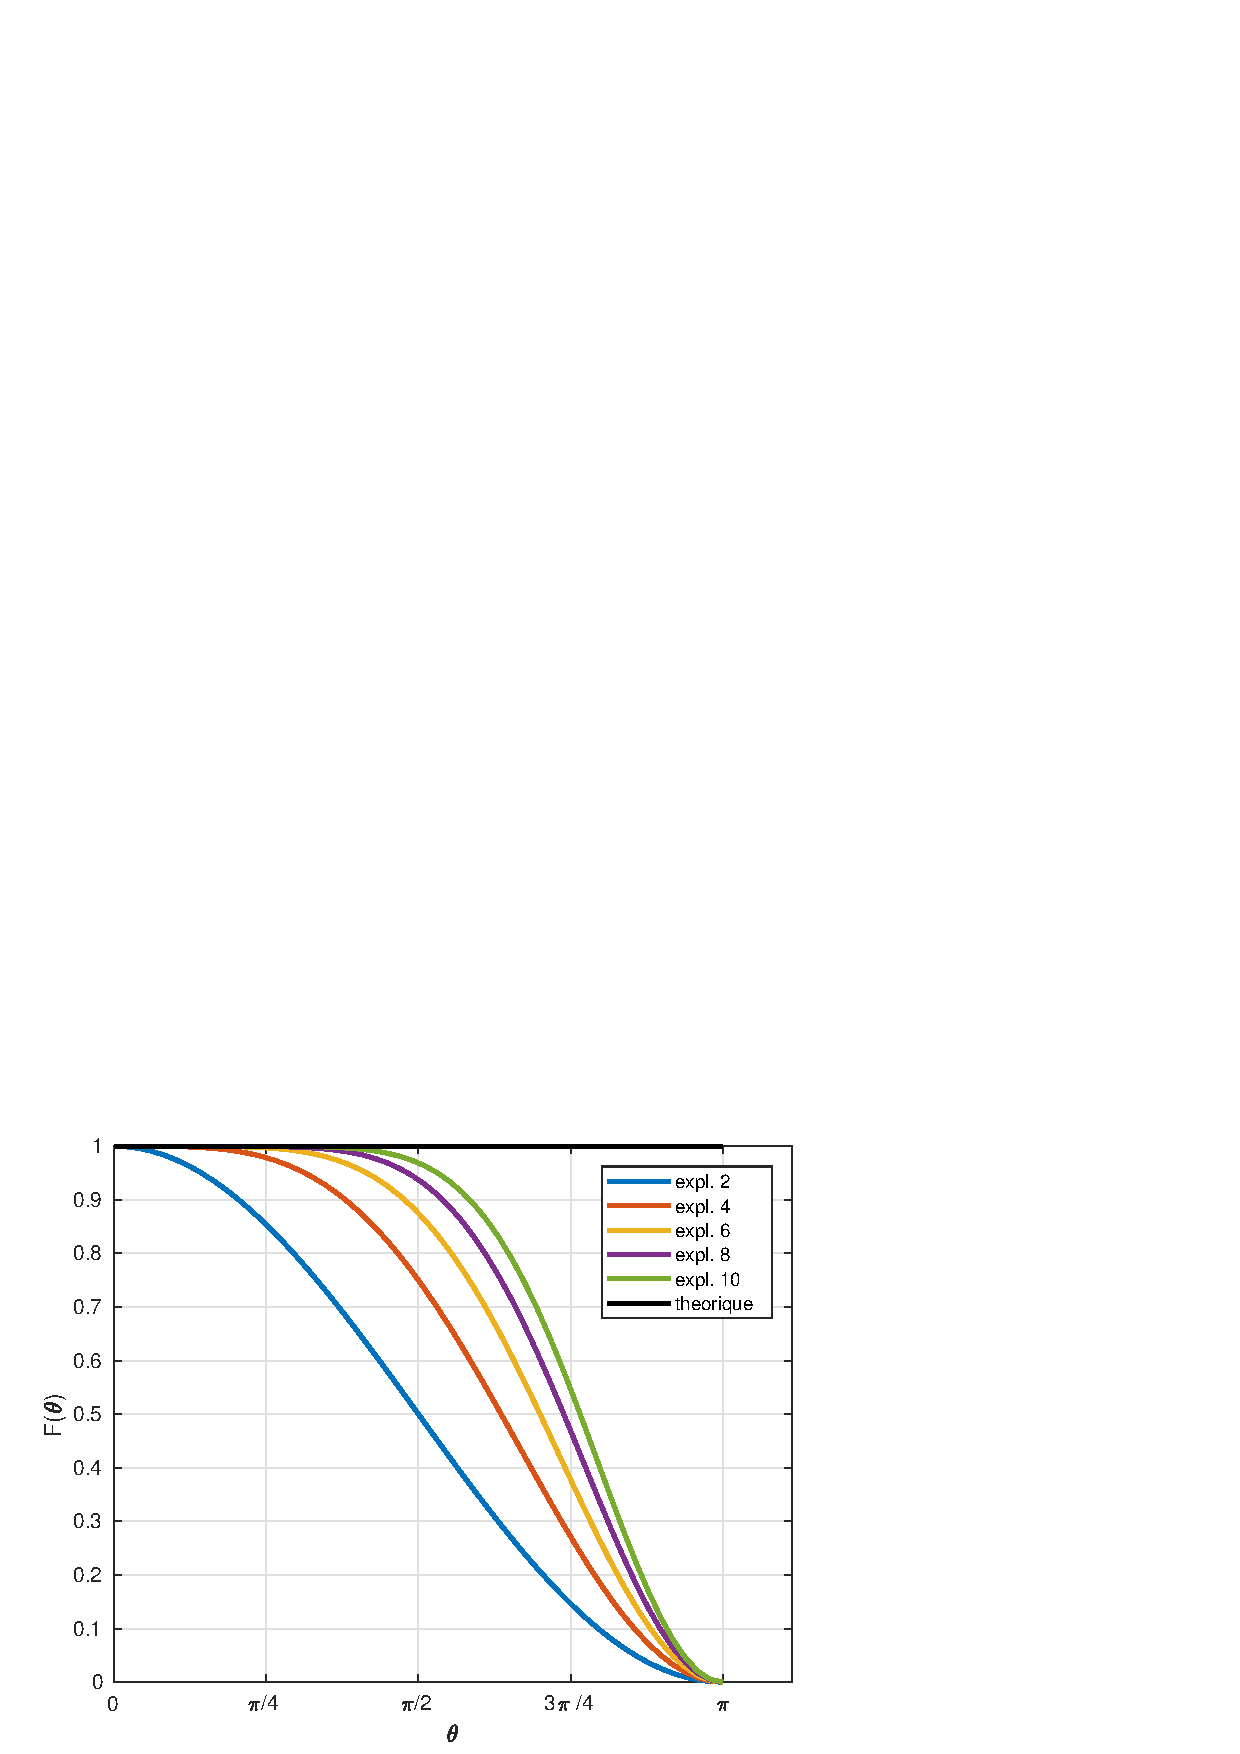
\includegraphics[scale=0.7]{freq_filter.png}
\end{center}
\caption{Fonction d'amplification $\beta$ pour les filtres explicites d'ordre 2, 4, 6, 8 et 10.}
\label{fig:freq_filter}
\end{figure}
Comme on s'y attendais, un filtre d'ordre élevé laisse passer un plus grand nombre de basses fréquences. Dans le tableau \ref{tab:filter_095}, on représente la fréquence $\theta_{0.95}$ maximale qui est conservée à $95\%$. Comme la fonction $\beta$ est strictement décroissante sur $[0,\pi]$, c'est une bijection de $[0,pi]$ dans $[0,1]$ et on a 
\begin{equation}
\theta_{0.95} = \beta^{-1}(0.95).
\end{equation}

\begin{table}
\begin{center}
\begin{tabular}{|c||c|}
\hline
\textbf{Ordre du filtre} & \textbf{Fréquence conservée à } $95\%$\\
\hline
\hline
$10$&$1.6695$\\
$8$&$1.5165$\\
$6$&$1.3045$\\
$4$&$0.9851$\\
$2$&$0.4510$\\
\hline
\end{tabular}
\end{center}
\caption{Fréquence conservée à $95\%$ en fonction de l'ordre du filtre.}
\label{tab:filter_095}
\end{table}

En pratique, cette fréquence $\theta_{0.95}$ est donnée en résolvant $\beta(\theta_{0.95})=0.95$ par 
\begin{equation}
\theta_{0.95} = \arccos \left[ 1-2 (0.05)^{1/F} \right].
\end{equation}
On remarque directement que la fonction $F \mapsto \theta_{0.95}$ est croissante, ce qui confirme que lorsque l'ordre de précision croit, $J$ croit et $\theta_{0.95}$ croit donc le filtre conserve un plus grand nombre de fréquences. De plus, 
\begin{equation}
\lim_{F \rightarrow \infty} \theta_{0.95} = \pi.
\end{equation}
Ce qui confirme la prise en compte d'un grand nombre de fréquence lorsque l'on augmente l'ordre du filtre. Cependant lorsque l'ordre du filtre augmente, l'effet de filtrage des hautes fréquences diminue.

Si $\mathfrak{u}$ est une fonction de grille, on pose $U$ et $\tilde{U}$ les vecteurs de $\mathbb{R}^N$ tel que
\begin{equation}
U = \begin{bmatrix}
\mathfrak{u}_1\\
\mathfrak{u}_2\\
\vdots \\
\mathfrak{u}_N\\
\end{bmatrix} \text{ et } 
\tilde{U} = \begin{bmatrix}
\mathcal{F}\mathfrak{u}_1\\
\mathcal{F}\mathfrak{u}_2\\
\vdots \\
\mathcal{F}\mathfrak{u}_N\\
\end{bmatrix}
\end{equation}
Alors $U$ et $\tilde{U}$ vérifient la relation
\begin{equation}
\tilde{U} = M F
\end{equation}
avec $M \in \mathcal{M}_N \left( \mathbb{R} \right)$ la matrice associée au filtrage des données en dimension 1 (dans le cas $F=2$):
\begin{equation}
M = \dfrac{1}{2}
\begin{bmatrix}
2a_0 & a_1 & a_2 &   &   &   & a_2 & a_1 \\ 
a_1 & 2 a_0 & a_1 & a_2 &   &   &   & a_2 \\ 
a_2 & a_1 & 2a_0 & a_1 & a_2 & (0) &   &   \\ 
  & a_2 & a_1 & 2a_0 & a_1 & a_2 &   &   \\ 
  &   & \ddots & \ddots & \ddots & \ddots & \ddots &   \\ 
  &   & (0) & a_2 & a_1 & 2 a_0 & a_1 & a_2 \\ 
a_2 &   &   &   & a_2 & a_1 & 2a_0 & a_1 \\ 
a_1 & a_2 &   &   &   & a_2 & a_1 & 2a_0
\end{bmatrix} 
\end{equation}
ou plus généralement 
\begin{equation}
M_{i,j} = \left\lbrace
\begin{array}{cl}
a_0 & \text{ si } i=j \\
\dfrac{1}{2} a_k & \text{ si } i+j \equiv k [N]\\
0 & \text{ sinon.}
\end{array}
\right.
\end{equation}
Il est clair que la matrice $M$ est symétrique.








\subsection{Opérateur de filtrage en géométrie cartésienne 2D}

Dans cette partie, nous utilisons toujours les notations de la section \ref{sec:notation_2D} en contexte périodique. Définissons les opérateurs de filtrage dans les directions $x$ et $y$ par
\begin{eqnarray*}
\mathcal{F}_x = \gsum_{k=0}^F a_k \dfrac{\tau_x^k + \tau_x^{-k}}{2} \\
\mathcal{F}_y = \gsum_{k=0}^F a_k \dfrac{\tau_y^k + \tau_y^{-k}}{2} \\
\end{eqnarray*}

Avec $(a_k)_{0 \leq k \leq F}$ vérifiant \ref{prop:filter_def}. Comme la géométrie est cartésienne, on remarque que 
\begin{equation}
\mathcal{F}_x \circ \mathcal{F}_y = \mathcal{F}_y \circ \mathcal{F}_x.
\end{equation}
Ce qui est faux lorsque la métrique n'est pas orthogonale.
La proposition \ref{prop:filter_def} permet de vérifier la consistance des opérateurs de filtrages.
Si $u : (x,y) \in \Omega \mapsto u(x,y) \in \mathbb{R}$ est fonction de $\mathcal{C}^{2F}$ alors :
\begin{eqnarray*}
\mathcal{F}_x u^*_{i,j} - u^*_{i,j} & = & C_xh^{2F}\\
\mathcal{F}_y u^*_{i,j} - u^*_{i,j} & = & C_yh^{2F}
\end{eqnarray*}
où $C_x$ et $C_y$ sont des constantes indépendantes de $h$.
En particulier, en composant les opérateurs, on peut définir un nouvel opérateur de filtrage. En effet  
\begin{equation}
(\mathcal{F}_x \circ \mathcal{F}_y) u_{i,j}^* - u_{i,j}^* = Ch^{2F}.
\end{equation}

L'écriture matricielle de l'opérateur de filtrage est donnée par la proposition suivante :
\begin{proposition}
Soit $\mathbf{u}$ une fonction de grille. Alors les opérateurs de filtrages s'écrivent à l'aide de matrices comme :
\begin{equation}
\left\lbrace
\begin{array}{rcl}
\text{vec}_2 (\mathcal{F}_x \mathbf{u}) & = & (Id \otimes M) \text{vec}_2 (\mathbf{u})\\
\text{vec}_2 (\mathcal{F}_y \mathbf{u}) & = & (M \otimes Id) \text{vec}_2 (\mathbf{u})\\
\end{array}
\right.
\end{equation}
\end{proposition}
Comme la matrice $M$ est symétrique, il est immédiat que $Id \otimes M$ et $M \otimes Id$ sont symétriques aussi.
















\section{Discrétisation temporelle}

La résolution numérique des équations considérées se fait par la méthode des lignes. Il s'agit de discrétiser dans un premier lieux les opérateurs spatiaux pour aboutir à une équations semi-discrétisée. Il ne reste que la dimension temporelle à considérer : il s'agit de la résolution numérique d'une équation aux dérivées ordinaires. Nous considérons ici des EDO de la forme
\begin{equation}
\dfrac{d q}{dt} = J_{\Delta} (q)
\label{eq:edo}
\end{equation}
avec la condition initiale $q(0)=q_0$. 
Ce choix de méthode est particulièrement pratique. La discrétisation spatiale et la discrétisation temporelle sont séparées, cela facilite le développement de nouvelles méthodes de discrétisations qui peuvent aisément être changées.

\subsection{Discrétisation de Runge-Kutta d'ordre 4}

Le schéma de résolution temporelle de référence que nous considérons est le schéma de Runge-Kutta d'ordre 4 (RK4). Si nous connaissons l'état de $q$ au temps $t^n = n \Delta t$ (que nous noterons $q^n$) alors nous cherchons à déterminer de façon explicite une valeur approchée de $q$ au temps $t^{n+1} = (n+1) \Delta t$. C'est à dire que nous cherchons $Q$ tel que
\begin{equation}
q^{n+1} = Q(q^n)
\end{equation}
Le schéma de Runge-Kutta d'ordre 4 s'écrit suivant l'algorithme \ref{alg:RK4}.

\begin{center}
\begin{minipage}[H]{12cm}
  \begin{algorithm}[H]
    \caption{: RK4}\label{alg:RK4}
    \begin{algorithmic}[1]
    \State $q^0 = q_0$ connu,
    \For{$n=0,1, \ldots$}
             \State  $K^{(1)} = J_{\Delta} \left( q^n \right)$,
             \State  $K^{(2)} = J_{\Delta} \left( q^n + \dfrac{\Delta t}{2} K^{(1)}\right)$,
             \State  $K^{(3)} = J_{\Delta} \left( q^n + \dfrac{\Delta t}{2} K^{(2)}\right)$,
             \State  $K^{(4)} = J_{\Delta} \left( q^n + \Delta t K^{(3)}\right)$,  
             \State  $q^{n+1} = q^n  + \dfrac{\Delta t}{6} \left( K^{(1)} + 2 K^{(2)} + 2 K^{(3)} + K^{(4)} \right)$.
            \EndFor
    \end{algorithmic}
    \end{algorithm}
\end{minipage}
\end{center}

\begin{theoreme}
La méthode de résolution RK4 donnée dans l'algorithme \ref{alg:RK4} définie une méthode de résolution de \ref{eq:edo} d'ordre 4. Si $q : t \in \mathbb{R}^+ \mapsto \mathbb{R}^N$ est une fonction de $\mathcal{C}^5$ et $q^n = q(n \Delta t)$ alors
\begin{equation}
q((n+1) \Delta t) - q^{n+1} = \mathcal{O} \left( \Delta t^5 \right)
\end{equation}

\end{theoreme}

\subsection{Stabilité}

\subsection{Schéma filtré}















\section{Equation d'advection 1D}

\subsection{Discrétisation}

\subsection{Consistance et Stabilité}

\subsection{Relations de conservations}
% CS.tex
\chapter{Cubed-Sphere}

\section{Construction}

\section{Coordonnées}

\subsection{Tenseur métrique}

\subsection{Symboles de Christophel}
% opsph.tex
% opérateurs sphériques sur la sphère

\chapter{Approximation des opérateurs sphériques sur la Cubed-sphere}

La résolution des équations de type Shallow-Water \REF la sphère $\mathbb{S}_a^2$ demande le calcul approché d'opérateurs classiques. Les opérateurs différentiels sont indispensables pour la discrétisation spatiale. On pense en particulier aux opérateurs divergence, gradient ou rotationnel. Dans cette section, nous les définissons sur la Cubed-sphere. 
Nous avons vu dans le cas 1D qu'un opérateur de filtrage peut être utile pour supprimer les modes de type "$+1/-1$" qui perturbent le calcul lors de la discrétisation en temps. Nous définissons les opérateurs de filtrages permettant d'aboutir au filtrage qui sera utilisé dans la discrétisation temporelle des équations.
Dans ce chapitre, les notations employées telles que $\xi$, $\eta$, $\alpha$, ... sont celles employées dans le chapitre \REF concernant la Cubed-sphere.

\section{Opérateurs différentiels sur la Cubed-sphere}

\subsection{Définition des opérateurs}
Soit $\mathbf{x}_{i,j}^k$ un point de la Cubed-sphere avec $- N/2 \leq i,j \leq N/2$ et $k = (I) \cdots (VI)$. Alors il existe deux grands cercles $C_i^{(1)}$ et $C_j^{(2)}$ deux grands cercles tels que $\mathbf{x}_{i,j}^k \in C_i^{(1)} \cap C^{(2)}_j$. $\alpha$ et $\beta$ sont respectivement les angles paramétrant $C_i^{(1)}$ et $C_j^{(2)}$.

On a définit le gradient en $\mathbf{x}_{i,j}^k$ par 
\begin{equation}
\nabla_T h = \dfrac{\partial h}{\partial \alpha}_{|C^{(2)}_j} \mathbf{g}^{\alpha} + \dfrac{\partial h}{\partial \beta}_{|C^{(1)}_i} \mathbf{g}^{\beta},
\end{equation}
où $h \mathbf{x} \in \mathbb{S}_a^2 \mapsto h(\mathbf{x})$ est une fonction régulière sur la sphère.

Le cercle $C_i^{(1)}$ (resp. $C_j^{(2)}$) est une isocline $\xi = \xi_i$ (resp $\eta = \eta_j$) constant. D'après le théorème \eqref{th:gradient_xieta}, le gradient est calculable via la formule
\begin{equation}
\nabla_T h = \dfrac{\partial h}{\partial \xi}_{|\eta_j} \mathbf{g}^{\xi} + \dfrac{\partial h}{\partial \eta}_{|\xi_i} \mathbf{g}^{\eta}.
\end{equation}
On remarque que si l'on est capable de calculer les dérivées partielles $\partial_{\xi}$ et $\partial_{\eta}$ le long des grands cercles, alors on est capable de déterminer la valeur du gradient.

Soit $\mathbf{v} : \mathbf{x} \in \mathbb{S}_a^2 \mapsto \mathbf{v}(\mathbf{x}) \in \mathbb{T}_{\mathbf{x}} \mathbb{S}_a^2$ un champ de vecteur tangent à la sphère. On définit la \textit{divergence} et le \textit{rotationnel} de $\mathbf{v}$ notés $\nabla_T \cdot \mathbf{v}$ et $\nabla_T \wedge \mathbf{v}$.

\begin{definition}
Soit $\mathbf{v} : \mathbf{x} \in \mathbb{S}_a^2 \mapsto \mathbf{v}(\mathbf{x}) \in \mathbb{T}_{\mathbf{x}} \mathbb{S}_a^2$ un champ de vecteur régulier sur la sphère. Alors la divergence de $\mathbf{v}$ en $\mathbf{x} \in C_i^{(1)} \cap C_j^{(2)}$ est donnée par
\begin{equation}
\nabla_T \cdot \mathbf{v} = \dfrac{\partial \mathbf{v}}{\partial \alpha}_{|C^{(2)}_j} \cdot \mathbf{g}^{\alpha} + \dfrac{\partial \mathbf{v}}{\partial \beta}_{|C^{(1)}_i} \cdot \mathbf{g}^{\beta}.
\end{equation}
\label{def:divergence}
La notation $\cdot$ désigne le produit scalaire usuel dans $\mathbb{R}^3$.
\end{definition}
Le rotationnel d'un champ de vecteurs représente la tendance des lignes de courant de $\mathbf{v}$ à tourner autour d'un point. Il est définit par

\begin{definition}
Soit $\mathbf{v} : \mathbf{x} \in \mathbb{S}_a^2 \mapsto \mathbf{v}(\mathbf{x}) \in \mathbb{T}_{\mathbf{x}} \mathbb{S}_a^2$ un champ de vecteur régulier sur la sphère. Alors le rotationnel de $\mathbf{v}$ en $\mathbf{x} \in C_i^{(1)} \cap C_j^{(2)}$ est donnée par
\begin{equation}
\nabla_T \wedge \mathbf{v} =  \mathbf{g}^{\alpha} \wedge \dfrac{\partial \mathbf{v}}{\partial \alpha}_{|C^{(2)}_j} + \mathbf{g}^{\beta} \wedge \dfrac{\partial \mathbf{v}}{\partial \beta}_{|C^{(1)}_i}
\end{equation}
où $\wedge$ désigne le produit vectoriel.
\label{def:rotationnel}
\end{definition}
La \textit{vorticité} du champ de vecteurs $\mathbf{v}$ est la composante normale du rotationnel :
\begin{equation}
\vort ( \mathbf{v} ) = \left( \nabla_T \wedge \mathbf{v} \right) \cdot \mathbf{k}
\label{eq:vorticité}
\end{equation}
avec $\mathbf{k}$ le vecteur unitaire extérieur à la sphère en $\mathbf{x} \in \mathbb{S}_a^2$, il vérifie l'égalité
\begin{equation}
\mathbf{k} = \dfrac{1}{a} \mathbf{x}.
\end{equation}

En utilisant la proposition \ref{prop: g_alpha g_beta fct de g_xi g_eta}, il est facile de montrer que des égalités permettant de calculer les opérateurs à l'aide des dérivées en $\xi$ et en $\eta$.

\begin{theoreme}
Soit $h : \mathbf{x} \in \mathbb{S}_a^2 \mapsto h(\mathbf{x})$ une fonction régulière et $\mathbf{v} : \mathbf{x} \in \mathbb{S}_a^2 \mapsto \mathbf{v}(\mathbf{x}) \in \mathbb{T}_{\mathbf{x}} \mathbb{S}_a^2$ un champ de vecteurs régulier. Alors en $\mathbf{x}_{i,j}^k$ un point de la Cubed-Sphere, les égalités suivantes sont satisfaites :
\begin{itemize}
\item \textbf{Gradient} :
\begin{equation}
\nabla_T h = \dfrac{\partial h}{\partial \xi}_{|\eta_j} \mathbf{g}^{\xi} + \dfrac{\partial h}{\partial \eta}_{|\xi_i} \mathbf{g}^{\eta},
\end{equation}

\item \textbf{Divergence} :
\begin{equation}
\nabla_T \cdot \mathbf{v} = \dfrac{\partial \mathbf{v}}{\partial \xi}_{|\eta_j} \cdot \mathbf{g}^{\xi} + \dfrac{\partial \mathbf{v}}{\partial \eta}_{|\xi_i} \cdot \mathbf{g}^{\eta},
\end{equation}

\item \textbf{Rotationel} :
\begin{equation}
\nabla_T \cdot \mathbf{v} = \mathbf{g}^{\xi} \wedge \dfrac{\partial \mathbf{v}}{\partial \xi}_{|\eta_j} + \mathbf{g}^{\eta} \wedge \dfrac{\partial \mathbf{v}}{\partial \eta}_{|\xi_i}.
\end{equation}
\end{itemize} 
\end{theoreme}

Pour calculer une valeur approchée des opérateurs gradient, divergence et rotationnel aux points du maillage de la Cubed-Sphere, il faut calculer une valeur approchée de la dérivée d'une fonction le long d'un grand cercle. C'est à dire, calculer $f_{\xi,i,j}$ et $f_{\eta,i,j}$ tels que 
\begin{equation}
\left\lbrace
\begin{array}{rl}
f_{\xi,i,j} \rightarrow \partial_{\xi} f ( \mathbf{x}_{i,j}^k) & \text{ lorsque } \Delta \xi \rightarrow 0\\
f_{\eta,i,j} \rightarrow \partial_{\eta} f ( \mathbf{x}_{i,j}^k) & \text{ lorsque } \Delta \eta \rightarrow 0
\end{array}
\right.
\end{equation}
La section suivante consiste à détailler une procédure pour calculer ces dérivées partielles approchées et à déterminer l'erreur effectuée lors du calcul.





\subsection{Approximation de dérivées sur les grands cercles}

On pose $f : \mathbf{x}\in \mathbb{S}_a^2 \mapsto f(\mathbf{x})$ la fonction que l'on souhaite dérivée le long des grands cercles aux points du maillage de la Cubed-Sphere.
Si $\mathbf{x}_{i,j}^k$ est un point de la Cubed-Sphere avec $k = (I) \cdots (VI)$, ainsi que $-N/2 \leq i,j \leq N/2$. On souhaite calculer une valeur approchée de 
$
\partial_{\xi} f (\mathbf{x}_{i,j}^k) \text{ et } \partial_{\xi} f (\mathbf{x}_{i,j}^k)
$.
On suppose par exemple $k = (I)$ mais la méthode est la même sur les autres panels. Alors il existe deux grands cercles de la Cubed-Sphere $C_i^{(1)}$ et $C_j^{(2)}$ tels que 
\begin{equation}
\mathbf{x}_{i,j}^k \in C_i^{(1)} \cap C^{(2)}_j.
\end{equation}
$C^{(1)}_i$ est une isoligne en $\xi = \xi_i$ constant et $C^{(2)}_j$ est une isoligne en $\eta = \eta_j$ constant.
Pour calculer une valeur approchée de $\partial_{\xi} f (\mathbf{x}_{i,j}^{(I)})$, on souhaite connaître toutes les valeurs de $f$ aux points équirépartis le long du cercle $C^{(2)}_j$. On pose $\mathbf{m}_p$ avec $0 \leq p \leq 4N-1$ les points de $C^{(2)}_j$ construits de la manière suivante :
\begin{itemize}
\item si $0 \leq p \leq N$ alors $\mathbf{m}_p = \mathbf{x}^{(I)}_{p-N/2,j}$, il s'agit des points du cercle $C^{(2)}_j$ associés au panel $(I)$ sur le maillage. Ils sont représentés par des ronds bleus sur les figures \ref{fig:patron_cs} et \ref{fig: panel II_interp},
\item si $N+1 \leq p \leq 2N-1$ alors les points ne font pas partis du maillages. Il s'agit des des points d'intersections de $C^{(2)}_j$ avec les isoligne $\xi = \xi_i^{(II)}$ du panel $(II)$. C'est à dire l'intersection de $C^{(2)}_j$ avec les cercles de $(II_{\beta})$. Ces points sont représentés par les carrés bleus dans les figures \ref{fig:patron_cs} et \ref{fig: panel II_interp}. Les coordonnées de ces points ont été calculées dans la partie \REF.
\item si $2N \leq p \leq 3N$ alors $\mathbf{m}_p = \mathbf{x}^{(III)}_{p-3N/2}$. Il s'agit des points de la Cubed-Sphere du panel $(III)$ représentés par des ronds bleus sur la figure \ref{fig:patron_cs},
\item si $3N+1 \leq p \leq 4N-1$ alors $\mathbf{m}_p$ est constitués des points d'intersections de $C^{(2)}_j$ avec les cercles de $(IV_{\beta})$. Il ne s'agit pas de points de la grille. Ces points sont représentés par les carrés bleus dans la figure \ref{fig:patron_cs}.
\end{itemize}

\begin{figure}
\begin{center}
\begin{tikzpicture}[scale=2.5]
	\foreach \x in {1,...,7}
		{ \draw [color=gray!70, line width=0.8pt] (0.125*\x,1) -- (0.125*\x,2) ;
		\draw [color=gray!30] (0,1+0.125*\x) -- (1,1+0.125*\x) ;
		\draw [color=gray!30] (1+0.125*\x,1) -- (1+0.125*\x,2) ;
		\draw [color=gray!30] (1,1+0.125*\x) -- (2,1+0.125*\x) ;
		\draw [color=gray!70, line width=0.8pt] (2+0.125*\x,1) -- (2+0.125*\x,2) ;
		\draw [color=gray!30] (2,1+0.125*\x) -- (3,1+0.125*\x) ;
		\draw [color=gray!30] (3+0.125*\x,1) -- (3+0.125*\x,2) ;
		\draw [color=gray!30] (3,1+0.125*\x) -- (4,1+0.125*\x) ;
		\draw [color=gray!30] (1+0.125*\x,0) -- (1+0.125*\x,1) ;
		\draw [color=gray!30] (1,0.125*\x) -- (2,0.125*\x) ;
		\draw [color=gray!30] (1+0.125*\x,2) -- (1+0.125*\x,3) ;		
		\draw [color=gray!30] (1,2+0.125*\x) -- (2,2+0.125*\x) ;
		}
	

	\draw [line width=0.6pt] (1,3) -- (2,3) ; 
	\draw [line width=0.6pt] (0,2) -- (4,2) ; 	
	\draw [line width=0.6pt] (0,1) -- (4,1) ; 
	\draw [line width=0.6pt] (1,0) -- (2,0) ; 
	
	\draw [line width=0.6pt] (0,2) -- (0,1) ;
	\draw [line width=0.6pt] (1,3) -- (1,0) ;
	\draw [line width=0.6pt] (2,3) -- (2,0) ;
	\draw [line width=0.6pt] (3,2) -- (3,1) ;
	\draw [line width=0.6pt] (4,2) -- (4,1) ; 
	
	\draw (0.7,1.1) node[above]{$(IV)$} ; 
	\draw (1.3,1.1) node[above]{$(I)$} ; 
	\draw (2.7,1.7) node[above]{$(II)$} ;
	\draw (3.3,1.7) node[above]{$(III)$} ;  
	\draw (1.7,2.7) node[above]{$(V)$} ;  
	\draw (1.3,0.7) node[above]{$(VI)$} ; 
	
	\draw [samples=100,domain=0:1,color=blue] plot({\x},{1.5-(2*0.125)*cos(180*\x)});
	\draw [samples=100,domain=1:2,color=blue] plot({\x},{1.5+2*0.125});
	\draw [samples=100,domain=1:2,color=blue] plot({\x+1},{1.5-2*0.125*cos(180*\x)});
	\draw [samples=100,domain=3:4,color=blue] plot({\x},{1.5-2*0.125});
	\draw [>=stealth, <-] (0.05,1.25) -- (0.3,0.5) ;
	\draw  (0.3,0.5) node[right] {iso-$\eta$} ;
	
	\draw [samples=100,domain=0:1,color=red] plot({1.5-2*0.125*cos(180*\x)},{\x});
	\draw [samples=100,domain=1:2,color=red] plot({1.5+2*0.125},{\x});
	\draw [samples=100,domain=1:2,color=red] plot({1.5-2*0.125*cos(180*\x)},{\x+1});
	\draw [samples=100,domain=1:2,color=red] plot({4-2*0.125},{\x});
	\draw [>=stealth, <-] (1.5,0.5) -- (2.2,0.4) ;
	\draw  (2.2,0.4) node[right] {iso-$\xi$} ;
	
	\draw  (0,1+2*0.125) node[color=blue] {$\bullet$} ;
	\draw (0,1+2*0.125) node {$\circ$} ;
	
	\foreach \k in {0,...,8}
		{\draw  (1+0.125*\k,1.5+2*0.125) node[color=blue] {$\bullet$} ;
	   	\draw (1+0.125*\k,1.5+2*0.125) node {$\circ$} ;
	   	\draw  (3+0.125*\k,1+2*0.125) node[color=blue] {$\bullet$} ;
	   	\draw (3+0.125*\k,1+2*0.125) node {$\circ$} ;
	   	}
	   	
	\foreach \x in {1,...,7}
		{\draw  ({0.125*\x},{1.5-2*0.125*cos(180*0.125*\x)}) node[color=blue] {\begin{tiny}$\blacksquare$\end{tiny}} ;
	   	\draw ({0.125*\x},{1.5-2*0.125*cos(180*0.125*\x)}) node {\begin{tiny}$\square$\end{tiny}} ;
	   	\draw  ({2+0.125*\x},{1.5-2*0.125*cos(180*0.125*\x+180)}) node[color=blue] {\begin{tiny}$\blacksquare$\end{tiny}} ;
	   	\draw  ({2+0.125*\x},{1.5-2*0.125*cos(180*0.125*\x+180)}) node {\begin{tiny}$\square$\end{tiny}} ;
	   	}
	   	
	\draw [>=stealth, <-] (0.25,1.75) -- (0.125,2.5) ;
	\draw [>=stealth, <-] (0.625,1.85) -- (0.125,2.5) ;
	\draw  (0.125,2.5) node[above] {Lignes d'interpolation} ;
\end{tikzpicture}
\caption{Les grands cercles associés aux panels $(I)$ et $(III)$ ne sont pas passent pas par des points du la Cubed-Sphere sur les panels $(II)$ et $(IV)$.}
\label{fig:patron_cs}
\end{center}
\end{figure}




\begin{figure}[htbp]
\begin{center}
\begin{tikzpicture}[scale=2.2]
	\draw [line width=0.8pt] (0,0) circle (1cm);
    \shade[ball color=blue!10!white,opacity=0.20] (0,0) circle (1cm);	
	
	\filldraw[draw=black,fill=blue!30!white,opacity=0.20]
	plot [smooth,domain=-35:35] ({0.7*cos(\x)},{sin(\x)})
	-- plot [smooth,domain=55:125] ({cos(\x)},{0.7*sin(\x)})
	-- plot [smooth,domain=150:215] ({0.7*cos(\x)},{sin(\x)})
	-- plot [smooth,domain=240:300] ({cos(\x)},{0.7*sin(\x)})
	-- cycle;	
	\draw [samples=100,domain=48:132, color=gray!50] plot({cos(\x)},{0.35*sin(\x)});
	\draw [samples=100,domain=48:132, color=gray!50] plot({cos(\x)},{-.35*sin(\x)});
	\draw [samples=100,domain=46:134, color=gray!50] plot({cos(\x)},{0.175*sin(\x)});
	\draw [samples=100,domain=46:134, color=gray!50] plot({cos(\x)},{-.175*sin(\x)});
	\draw [samples=100,domain=50:130, color=gray!50] plot({cos(\x)},{0.525*sin(\x)});
	\draw [samples=100,domain=50:130, color=gray!50] plot({cos(\x)},{-.525*sin(\x)});
	\draw [samples=100,domain=45:135, color=gray!50] plot({cos(\x)},{0*sin(\x)});

	\draw [rotate=90, samples=100,domain=48:132, color=gray, line width=0.6pt] plot({cos(\x)},{0.35*sin(\x)});
	\draw [rotate=90, samples=100,domain=48:132, color=gray, line width=0.6pt] plot({cos(\x)},{-.35*sin(\x)});
	\draw [rotate=90, samples=100,domain=46:134, color=gray, line width=0.6pt] plot({cos(\x)},{0.175*sin(\x)});
	\draw [rotate=90, samples=100,domain=46:134, color=gray, line width=0.6pt] plot({cos(\x)},{-.175*sin(\x)});
	\draw [rotate=90, samples=100,domain=50:130, color=gray, line width=0.6pt] plot({cos(\x)},{0.525*sin(\x)});
	\draw [rotate=90, samples=100,domain=50:130, color=gray, line width=0.6pt] plot({cos(\x)},{-.525*sin(\x)});
	\draw [rotate=90, samples=100,domain=45:135, color=gray, line width=0.6pt] plot({cos(\x)},{0*sin(\x)});

	\filldraw[draw=black,fill=red!30!white,opacity=0.20]
	plot [smooth,domain=145:215] ({.7*cos(\x)},{sin(\x)})
	-- plot [smooth] (-.573,-.573) -- (-.707,-.707)
	-- plot [smooth,domain=215:145] ({cos(\x)},{sin(\x)})
	-- plot [smooth] (-.707,.707) -- (-.573,.573)
	-- cycle;	
	\draw [line width=0.8pt] (-.573,-.573) -- (-.707,-.707) ;
	\draw [line width=0.8pt] (-.573,.573) -- (-.707,.707) ;
	\draw [color=gray!50] (-.669,.260) -- (-.9321,.3622) ;
	\draw [color=gray!50] (-.669,-.260) -- (-.9321,-.3622) ;
	\draw [color=gray!50] (-.6946,.1259) -- (-.9840,.1783) ;
	\draw [color=gray!50] (-.6946,-.1259) -- (-.9840,-.1783) ;
	\draw [color=gray!50] (-.6427,.4022) -- (-.8477,.5305) ;
	\draw [color=gray!50] (-.6427,-.4022) -- (-.8477,-.5305) ;
	\draw [color=gray!50] (-.707,0) -- (-1,0) ;
	\draw [samples=100,domain=141:219, color=gray!50] plot({0.8*cos(\x)},{sin(\x)});
	\draw [samples=100,domain=138:222, color=gray!50] plot({0.9*cos(\x)},{sin(\x)});
	
	\filldraw[draw=black,fill=green!30!white,opacity=0.20]
	plot [smooth,domain=55:125] ({cos(\x)},{0.7*sin(\x)})
	-- plot [smooth] (-.573,.573) -- (-.707,.707)
	-- plot [smooth,domain=125:55] ({cos(\x)},{sin(\x)})
	-- plot [smooth] (.707,.707) -- (.573,.573)
	-- cycle;	
	\draw [line width=0.8pt] (-.573,.573) -- (-.707,.707) ;
	\draw [line width=0.8pt] (.707,.707) -- (.573,.573) ;
	\draw [rotate=-90,color=gray!50] (-.669,.260) -- (-.9321,.3622) ;
	\draw [rotate=-90,color=gray!50] (-.669,-.260) -- (-.9321,-.3622) ;
	\draw [rotate=-90,color=gray!50] (-.6946,.1259) -- (-.9840,.1783) ;
	\draw [rotate=-90,color=gray!50] (-.6946,-.1259) -- (-.9840,-.1783) ;
	\draw [rotate=-90,color=gray!50] (-.6427,.4022) -- (-.8477,.5305) ;
	\draw [rotate=-90,color=gray!50] (-.6427,-.4022) -- (-.8477,-.5305) ;
	\draw [rotate=-90,color=gray!50] (-.707,0) -- (-1,0) ;
	\draw [rotate=-90,samples=100,domain=141:219, color=gray!50] plot({0.8*cos(\x)},{sin(\x)});
	\draw [rotate=-90,samples=100,domain=138:222, color=gray!50] plot({0.9*cos(\x)},{sin(\x)});
	
	\filldraw[draw=black,fill=yellow!30!white,opacity=0.20]
	plot [smooth,domain=55:125] ({cos(\x)},{-.7*sin(\x)})
	-- plot [smooth] (-.573,-.573) -- (-.707,-.707)
	-- plot [smooth,domain=125:55] ({cos(\x)},{-sin(\x)})
	-- plot [smooth] (.707,-.707) -- (.573,-.573)
	-- cycle;	
	\draw [line width=0.8pt] (-.573,-.573) -- (-.707,-.707) ;
	\draw [line width=0.8pt] (.707,-.707) -- (.573,-.573) ;
	\draw [rotate=90,color=gray!50] (-.669,.260) -- (-.9321,.3622) ;
	\draw [rotate=90,color=gray!50] (-.669,-.260) -- (-.9321,-.3622) ;
	\draw [rotate=90,color=gray!50] (-.6946,.1259) -- (-.9840,.1783) ;
	\draw [rotate=90,color=gray!50] (-.6946,-.1259) -- (-.9840,-.1783) ;
	\draw [rotate=90,color=gray!50] (-.6427,.4022) -- (-.8477,.5305) ;
	\draw [rotate=90,color=gray!50] (-.6427,-.4022) -- (-.8477,-.5305) ;
	\draw [rotate=90,color=gray!50] (-.707,0) -- (-1,0) ;
	\draw [rotate=90,samples=100,domain=141:219, color=gray!50] plot({0.8*cos(\x)},{sin(\x)});
	\draw [rotate=90,samples=100,domain=138:222, color=gray!50] plot({0.9*cos(\x)},{sin(\x)});
	
	\draw [rotate=180,color=gray!50] (-.669,.260) -- (-.9321,.3622) ;
	\draw [rotate=180,color=gray!50] (-.669,-.260) -- (-.9321,-.3622) ;
	\draw [rotate=180,color=gray!50] (-.6946,.1259) -- (-.9840,.1783) ;
	\draw [rotate=180,color=gray!50] (-.6946,-.1259) -- (-.9840,-.1783) ;
	\draw [rotate=180,color=gray!50] (-.6427,.4022) -- (-.8477,.5305) ;
	\draw [rotate=180,color=gray!50] (-.6427,-.4022) -- (-.8477,-.5305) ;
	\draw [rotate=180,color=gray!50] (-.707,0) -- (-1,0) ;
	\draw [rotate=180,samples=100,domain=141:219, color=gray!50] plot({0.8*cos(\x)},{sin(\x)});
	\draw [rotate=180,samples=100,domain=138:222, color=gray!50] plot({0.9*cos(\x)},{sin(\x)});
	
	\draw [samples=100,domain=55:125, line width=0.8pt] plot({cos(\x)},{0.7*sin(\x)});
	\draw [samples=100,domain=55:125, line width=0.8pt] plot({cos(\x)},{-.7*sin(\x)});
	\draw [samples=100,domain=145:215, line width=0.8pt] plot({.7*cos(\x)},{sin(\x)}); 
	\draw [samples=100,domain=145:215, line width=0.8pt] plot({-.7*cos(\x)},{sin(\x)}); 
	
	\draw [color=blue] (-.9321,.3622) -- (.9321,-.3622) ;
	\draw  (-.9321,.3622) node[color=blue] {$\bullet$} ;
	\draw (-.9321,.3622) node {$\circ$} ;	
	\draw  (.9321,-.3622) node[color=blue] {$\bullet$} ;
	\draw (.9321,-.3622) node {$\circ$} ;
	\draw  (-.85,0.3886*.85) node[color=blue] {$\bullet$} ;
	\draw (-.85,0.3886*.85) node {$\circ$} ;	
	\draw (.85,-0.3886*.85) node[color=blue] {$\bullet$} ;
	\draw (.85,-0.3886*.85) node {$\circ$} ;	
	\draw  (-.76,0.3886*.76) node[color=blue] {$\bullet$} ;
	\draw (-.76,0.3886*.76) node {$\circ$} ;	
	\draw (.76,-0.3886*.76) node[color=blue] {$\bullet$} ;
	\draw (.76,-0.3886*.76) node {$\circ$} ;
	\draw  (-.68,0.3886*.68) node[color=blue] {$\bullet$} ;
	\draw (-.68,0.3886*.68) node {$\circ$} ;	
	\draw (.68,-0.3886*.68) node[color=blue] {$\bullet$} ;
	\draw (.68,-0.3886*.68) node {$\circ$} ;	
	\draw (-.52,0.3886*.52) node[color=blue] {\begin{tiny}$\blacksquare$ \end{tiny}} ;
	\draw (-.52,0.3886*.52) node {\begin{tiny}$\square$ \end{tiny}} ;
	\draw (.52,-0.3886*.52) node[color=blue] {\begin{tiny}$\blacksquare$ \end{tiny}} ;
	\draw (.52,-0.3886*.52) node {\begin{tiny}$\square$ \end{tiny}} ;
	\draw (-.36,0.3886*.36) node[color=blue] {\begin{tiny}$\blacksquare$ \end{tiny}} ;
	\draw (-.36,0.3886*.36) node {\begin{tiny}$\square$ \end{tiny}} ;
	\draw (.36,-0.3886*.36) node[color=blue] {\begin{tiny}$\blacksquare$ \end{tiny}} ;
	\draw (.36,-0.3886*.36) node {\begin{tiny}$\square$ \end{tiny}} ;
	\draw (-.18,0.3886*.18) node[color=blue] {\begin{tiny}$\blacksquare$ \end{tiny}} ;
	\draw (-.18,0.3886*.18) node {\begin{tiny}$\square$ \end{tiny}} ;
	\draw (.18,-0.3886*.18) node[color=blue] {\begin{tiny}$\blacksquare$ \end{tiny}} ;
	\draw (.18,-0.3886*.18) node {\begin{tiny}$\square$ \end{tiny}} ;
	\draw (0,0) node[color=blue] {\begin{tiny}$\blacksquare$ \end{tiny}} ;
	\draw (0,0) node {\begin{tiny}$\square$ \end{tiny}} ;
	
	\draw [>=stealth, <-] (.33,.35) -- (.7,1) ;
	\draw [>=stealth, <-] (0,.4) -- (.7,1) ;
	\draw  (0.7,1) node[right] {Lignes d'interpolations} ;
	
	\draw  (0,-1.7) node {Panel (II)} ;

\end{tikzpicture}
\end{center}
\caption{La ligne bleue représente une isoligne $\eta=\eta_j$ du panel $(I)$ vue depuis le panel $(II)$. les cercles bleus représentent des points de la Cubed-Sphere contenues dans l'isoligne $\eta=\eta_j$, les carrés bleus sont des points de l'isoligne $\eta=\eta_j$ qui ne sont pas sur la Cubed-Sphere.}
\label{fig: panel II_interp}
\end{figure}  

La périodicité sur les grands cercles permet d'assurer que $\mathbf{m}_p = \mathbf{m}_{p+4N}$ pour tout $p \in \mathbb{Z}$. De plus, la construction de la Cubed-Sphere, permet d'assurer un paramétrage du grand cercle $C^{(2)}_j$. Chaque point est associé à des coordonnées $(\xi_p, \eta_p)$. Les valeurs de $\xi_p$ donnent un paramétrage des points $\mathbf{m}_p$ le long du grand cercle. On a de plus
\begin{equation}
\xi_{p+1} = \xi_p + \Delta \xi
\end{equation}
Si $f_p = f(\mathbf{m}_p)$ est connue pour tout $p$ vérifiant $0 \leq p \leq 4N-1$ alors on peut calculer la dérivée approchée $f_{\xi,i,j}^k$ de $\partial_{\xi}f(\mathbf{x}_{i,j}^k)$ à l'ordre $4$ grâce à la formule de dérivation hermitienne \eqref{def:herm_4}
\begin{equation}
f_{\xi,i,j}^k = \delta_{\xi}^H f_p.
\end{equation}
Cependant, les valeurs de $f_p$ ne sont pas toutes connues car les points $\mathbf{m}_p$ ne sont pas des points du maillages lorsque $N+1 \leq p \leq 2N-1$ ou $3N+4 \leq p \leq 4N-1$. Il faut donc construire un procéder permettant d'obtenir des valeurs en ces points. Le procédé utilisé dans ce travail est basé sur une interpolation à l'aide de Splines Cubiques.

On souhaite calculer une valeur $f_p$ approchant $f(\mathbf{m}_p)$ avec $N+1 \leq p \leq 2N-1$ ou $3N+4 \leq p \leq 4N-1$. Dans ce cadre, $\mathbf{m}_p$ n'est pas un point de la Cubed-Sphere. Cependant on sait que 
\begin{equation}
\mathbf{m}_p \in C^{(2)}_j \cap C
\end{equation} 
où $C^{(2)}_j$ est une isoligne pour $\eta = \eta_j$ constant pour le panel $(I)$ et $C$ est une isoligne $\xi$ constant pour le panel $(II)$ (si $N+1 \leq p \leq 2N-1$) ou pour le panel $(IV)$ si $3N+4 \leq p \leq 4N-1$ (lignes en gras sur les figures \ref{fig:patron_cs}.et \ref{fig: panel II_interp}).
La méthode consiste à utiliser les points de la Cubed-Sphere présents sur le cercle $C$ pour construire une fonction d'interpolation de type Spline Cubique puis d'évaluer cette fonction au point du maillage $\mathbf{m}_p$. Si on note $P_C$ la fonction d'interpolation en question, on a alors $f_p = P_C (\mathbf{m}_p)$. L'interpolation s'effectuant sur un grand cercle, il s'agit d'une fonction d'interpolation 1D. De plus, cette fonction étant issue des splines cubiques, on a :
\begin{equation}
f_p = P_C(\mathbf{m}_p) = f(\mathbf{m}_p) + \mathcal{O}(\Delta \eta^4).
\end{equation}
La fonction $P_C$ ne dépend pas du point $\mathbf{m}_p$ mais uniquement des données aux points de la Cubed-Sphere sur le panel choisit et le long de $C$ (Voir figure \ref{fig: panel II_interp2}).

\begin{figure}[htbp]
\begin{center}
\begin{tikzpicture}[scale=2.2]
	\draw [line width=0.8pt] (0,0) circle (1cm);
    \shade[ball color=blue!10!white,opacity=0.20] (0,0) circle (1cm);	
	
	\filldraw[draw=black,fill=blue!30!white,opacity=0.20]
	plot [smooth,domain=-35:35] ({0.7*cos(\x)},{sin(\x)})
	-- plot [smooth,domain=55:125] ({cos(\x)},{0.7*sin(\x)})
	-- plot [smooth,domain=150:215] ({0.7*cos(\x)},{sin(\x)})
	-- plot [smooth,domain=240:300] ({cos(\x)},{0.7*sin(\x)})
	-- cycle;	
	\draw [samples=100,domain=48:132, color=gray!50] plot({cos(\x)},{0.35*sin(\x)});
	\draw [samples=100,domain=48:132, color=gray!50] plot({cos(\x)},{-.35*sin(\x)});
	\draw [samples=100,domain=46:134, color=gray!50] plot({cos(\x)},{0.175*sin(\x)});
	\draw [samples=100,domain=46:134, color=gray!50] plot({cos(\x)},{-.175*sin(\x)});
	\draw [samples=100,domain=50:130, color=gray!50] plot({cos(\x)},{0.525*sin(\x)});
	\draw [samples=100,domain=50:130, color=gray!50] plot({cos(\x)},{-.525*sin(\x)});
	\draw [samples=100,domain=45:135, color=gray!50] plot({cos(\x)},{0*sin(\x)});

	\draw [rotate=90, samples=100,domain=48:132, color=gray!50] plot({cos(\x)},{0.35*sin(\x)});
	\draw [rotate=90, samples=100,domain=48:132, color=gray!50] plot({cos(\x)},{-.35*sin(\x)});
	\draw [rotate=90, samples=100,domain=46:134, color=green, line width=0.6pt] plot({cos(\x)},{-.175*sin(\x)});
	\draw [rotate=90, samples=100,domain=46:134, color=gray!50] plot({cos(\x)},{0.175*sin(\x)});
	\draw [rotate=90, samples=100,domain=50:130, color=gray!50] plot({cos(\x)},{0.525*sin(\x)});
	\draw [rotate=90, samples=100,domain=50:130, color=gray!50] plot({cos(\x)},{-.525*sin(\x)});
	\draw [rotate=90, samples=100,domain=45:135, color=gray!50] plot({cos(\x)},{0*sin(\x)});

	\filldraw[draw=black,fill=red!30!white,opacity=0.20]
	plot [smooth,domain=145:215] ({.7*cos(\x)},{sin(\x)})
	-- plot [smooth] (-.573,-.573) -- (-.707,-.707)
	-- plot [smooth,domain=215:145] ({cos(\x)},{sin(\x)})
	-- plot [smooth] (-.707,.707) -- (-.573,.573)
	-- cycle;	
	\draw [line width=0.8pt] (-.573,-.573) -- (-.707,-.707) ;
	\draw [line width=0.8pt] (-.573,.573) -- (-.707,.707) ;
	\draw [color=gray!50] (-.669,.260) -- (-.9321,.3622) ;
	\draw [color=gray!50] (-.669,-.260) -- (-.9321,-.3622) ;
	\draw [color=gray!50] (-.6946,.1259) -- (-.9840,.1783) ;
	\draw [color=gray!50] (-.6946,-.1259) -- (-.9840,-.1783) ;
	\draw [color=gray!50] (-.6427,.4022) -- (-.8477,.5305) ;
	\draw [color=gray!50] (-.6427,-.4022) -- (-.8477,-.5305) ;
	\draw [color=gray!50] (-.707,0) -- (-1,0) ;
	\draw [samples=100,domain=141:219, color=gray!50] plot({0.8*cos(\x)},{sin(\x)});
	\draw [samples=100,domain=138:222, color=gray!50] plot({0.9*cos(\x)},{sin(\x)});
	
	\filldraw[draw=black,fill=green!30!white,opacity=0.20]
	plot [smooth,domain=55:125] ({cos(\x)},{0.7*sin(\x)})
	-- plot [smooth] (-.573,.573) -- (-.707,.707)
	-- plot [smooth,domain=125:55] ({cos(\x)},{sin(\x)})
	-- plot [smooth] (.707,.707) -- (.573,.573)
	-- cycle;	
	\draw [line width=0.8pt] (-.573,.573) -- (-.707,.707) ;
	\draw [line width=0.8pt] (.707,.707) -- (.573,.573) ;
	\draw [rotate=-90,color=gray!50] (-.669,.260) -- (-.9321,.3622) ;
	\draw [rotate=-90,color=gray!50] (-.669,-.260) -- (-.9321,-.3622) ;
	\draw [rotate=-90,color=gray!50] (-.6946,.1259) -- (-.9840,.1783) ;
	\draw [rotate=-90,color=gray!50] (-.6946,-.1259) -- (-.9840,-.1783) ;
	\draw [rotate=-90,color=gray!50] (-.6427,.4022) -- (-.8477,.5305) ;
	\draw [rotate=-90,color=gray!50] (-.6427,-.4022) -- (-.8477,-.5305) ;
	\draw [rotate=-90,color=gray!50] (-.707,0) -- (-1,0) ;
	\draw [rotate=-90,samples=100,domain=141:219, color=gray!50] plot({0.8*cos(\x)},{sin(\x)});
	\draw [rotate=-90,samples=100,domain=138:222, color=gray!50] plot({0.9*cos(\x)},{sin(\x)});
	
	\filldraw[draw=black,fill=yellow!30!white,opacity=0.20]
	plot [smooth,domain=55:125] ({cos(\x)},{-.7*sin(\x)})
	-- plot [smooth] (-.573,-.573) -- (-.707,-.707)
	-- plot [smooth,domain=125:55] ({cos(\x)},{-sin(\x)})
	-- plot [smooth] (.707,-.707) -- (.573,-.573)
	-- cycle;	
	\draw [line width=0.8pt] (-.573,-.573) -- (-.707,-.707) ;
	\draw [line width=0.8pt] (.707,-.707) -- (.573,-.573) ;
	\draw [rotate=90,color=gray!50] (-.669,.260) -- (-.9321,.3622) ;
	\draw [rotate=90,color=gray!50] (-.669,-.260) -- (-.9321,-.3622) ;
	\draw [rotate=90,color=gray!50] (-.6946,.1259) -- (-.9840,.1783) ;
	\draw [rotate=90,color=gray!50] (-.6946,-.1259) -- (-.9840,-.1783) ;
	\draw [rotate=90,color=gray!50] (-.6427,.4022) -- (-.8477,.5305) ;
	\draw [rotate=90,color=gray!50] (-.6427,-.4022) -- (-.8477,-.5305) ;
	\draw [rotate=90,color=gray!50] (-.707,0) -- (-1,0) ;
	\draw [rotate=90,samples=100,domain=141:219, color=gray!50] plot({0.8*cos(\x)},{sin(\x)});
	\draw [rotate=90,samples=100,domain=138:222, color=gray!50] plot({0.9*cos(\x)},{sin(\x)});
	
	\draw [rotate=180,color=gray!50] (-.669,.260) -- (-.9321,.3622) ;
	\draw [rotate=180,color=gray!50] (-.669,-.260) -- (-.9321,-.3622) ;
	\draw [rotate=180,color=gray!50] (-.6946,.1259) -- (-.9840,.1783) ;
	\draw [rotate=180,color=gray!50] (-.6946,-.1259) -- (-.9840,-.1783) ;
	\draw [rotate=180,color=gray!50] (-.6427,.4022) -- (-.8477,.5305) ;
	\draw [rotate=180,color=gray!50] (-.6427,-.4022) -- (-.8477,-.5305) ;
	\draw [rotate=180,color=gray!50] (-.707,0) -- (-1,0) ;
	\draw [rotate=180,samples=100,domain=141:219, color=gray!50] plot({0.8*cos(\x)},{sin(\x)});
	\draw [rotate=180,samples=100,domain=138:222, color=gray!50] plot({0.9*cos(\x)},{sin(\x)});
	
	\draw [samples=100,domain=55:125, line width=0.8pt] plot({cos(\x)},{0.7*sin(\x)});
	\draw [samples=100,domain=55:125, line width=0.8pt] plot({cos(\x)},{-.7*sin(\x)});
	\draw [samples=100,domain=145:215, line width=0.8pt] plot({.7*cos(\x)},{sin(\x)}); 
	\draw [samples=100,domain=145:215, line width=0.8pt] plot({-.7*cos(\x)},{sin(\x)}); 
	
	\draw (.175,0) node[color=green] {$\bullet$} ;
	\draw (.175,0) node {$\circ$} ;
	\draw (.17,.17) node[color=green] {$\bullet$} ;
	\draw (.17,.17) node {$\circ$} ;
	\draw (.165,.335) node[color=green] {$\bullet$} ;
	\draw (.165,.335) node {$\circ$} ;
	\draw (.155,.52) node[color=green] {$\bullet$} ;
	\draw (.155,.52) node {$\circ$} ;
	\draw (.14,.684) node[color=green] {$\bullet$} ;
	\draw (.14,.684) node {$\circ$} ;
	\draw (.17,-.17) node[color=green] {$\bullet$} ;
	\draw (.17,-.17) node {$\circ$} ;
	\draw (.165,-.335) node[color=green] {$\bullet$} ;
	\draw (.165,-.335) node {$\circ$} ;
	\draw (.155,-.52) node[color=green] {$\bullet$} ;
	\draw (.155,-.52) node {$\circ$} ;
	\draw (.14,-.684) node[color=green] {$\bullet$} ;
	\draw (.14,-.684) node {$\circ$} ;
	
	\draw [>=stealth, <-] (0.17,.4) -- (.7,1) ;
	\draw  (0.7,1) node[right] {Ligne d'interpolation} ;
	\draw [>=stealth, <-] (.165,-.335) -- (.7,-1) ;
	\draw  (0.7,-1) node[right] {Point d'interpolation} ;
	
	
	
	
	
	
	\draw [color=blue] (-.9321,.3622) -- (.9321,-.3622) ;
	\draw  (-.9321,.3622) node[color=blue] {$\bullet$} ;
	\draw (-.9321,.3622) node {$\circ$} ;	
	\draw  (.9321,-.3622) node[color=blue] {$\bullet$} ;
	\draw (.9321,-.3622) node {$\circ$} ;
	\draw  (-.85,0.3886*.85) node[color=blue] {$\bullet$} ;
	\draw (-.85,0.3886*.85) node {$\circ$} ;	
	\draw (.85,-0.3886*.85) node[color=blue] {$\bullet$} ;
	\draw (.85,-0.3886*.85) node {$\circ$} ;	
	\draw  (-.76,0.3886*.76) node[color=blue] {$\bullet$} ;
	\draw (-.76,0.3886*.76) node {$\circ$} ;	
	\draw (.76,-0.3886*.76) node[color=blue] {$\bullet$} ;
	\draw (.76,-0.3886*.76) node {$\circ$} ;
	\draw  (-.68,0.3886*.68) node[color=blue] {$\bullet$} ;
	\draw (-.68,0.3886*.68) node {$\circ$} ;	
	\draw (.68,-0.3886*.68) node[color=blue] {$\bullet$} ;
	\draw (.68,-0.3886*.68) node {$\circ$} ;	
	\draw (-.52,0.3886*.52) node[color=blue] {\begin{tiny}$\blacksquare$ \end{tiny}} ;
	\draw (-.52,0.3886*.52) node {\begin{tiny}$\square$ \end{tiny}} ;
	\draw (.52,-0.3886*.52) node[color=blue] {\begin{tiny}$\blacksquare$ \end{tiny}} ;
	\draw (.52,-0.3886*.52) node {\begin{tiny}$\square$ \end{tiny}} ;
	\draw (-.36,0.3886*.36) node[color=blue] {\begin{tiny}$\blacksquare$ \end{tiny}} ;
	\draw (-.36,0.3886*.36) node {\begin{tiny}$\square$ \end{tiny}} ;
	\draw (.36,-0.3886*.36) node[color=blue] {\begin{tiny}$\blacksquare$ \end{tiny}} ;
	\draw (.36,-0.3886*.36) node {\begin{tiny}$\square$ \end{tiny}} ;
	\draw (-.18,0.3886*.18) node[color=blue] {\begin{tiny}$\blacksquare$ \end{tiny}} ;
	\draw (-.18,0.3886*.18) node {\begin{tiny}$\square$ \end{tiny}} ;
	\draw (.18,-0.3886*.18) node[color=blue] {\begin{tiny}$\blacksquare$ \end{tiny}} ;
	\draw (.18,-0.3886*.18) node {\begin{tiny}$\square$ \end{tiny}} ;
	\draw (0,0) node[color=blue] {\begin{tiny}$\blacksquare$ \end{tiny}} ;
	\draw (0,0) node {\begin{tiny}$\square$ \end{tiny}} ;
	
	\draw  (0,-1.7) node {Panel (II)} ;

\end{tikzpicture}
\end{center}
\caption{La ligne bleue représente une isoligne $\eta=\eta_j$ du panel $(I)$ vue depuis le panel $(II)$. les cercles bleus représentent des points de la Cubed-Sphere contenues dans l'isoligne $\eta=\eta_j$, les carrés bleus sont des points de l'isoligne $\eta=\eta_j$ qui ne sont pas sur la Cubed-Sphere. En vert, une portion du grand cercle utilisé pour l'interpolation.}
\label{fig: panel II_interp2}
\end{figure}  

Le procédé est symétrique pour reconstruire les données sur un grand cercle $C_i^{(1)}$ ou le grand cercle d'un autre panel.
Une fois les données $(f_p)_{0 \leq p \leq 4N-1}$ construites, on peut calculer l'approximation de la dérivée grâce à $\partial_{\xi} f_p \approx \delta_{\Delta \xi}^H f_p$
que l'on restreint aux points du maillage par 
\begin{equation}
\left\lbrace
\begin{array}{rcl}
f_{\xi,i,j}^{(I)} & = & \delta_{\Delta \xi}^H f_{i-N/2}\\
f_{\xi,i,j}^{(III)} & = & \delta_{\Delta \xi}^H f_{i+3N/2}
\end{array}
\right.
\text{ pour } C^{(2)}_j \text{ fixé.}
\end{equation}

Finalement, le procédé total de calcul des dérivées hermitienne est $\xi$ sur un panel $k$ est donné par l'algorithme \ref{alg:deltaxi}.

\begin{center}
\begin{minipage}[H]{12cm}
  \begin{algorithm}[H]
    \caption{: Calcul de $f_{\xi, i, j}^{(I)}$ et $f_{\xi, i, j}^{(III)}$}\label{alg:deltaxi}
    \begin{algorithmic}[1]
    \For{ $j=-N/2, \ldots , N/2$, }
    \State pour un grand cercle $C_j^{(2)}$ fixé,
    \For{$p=0,1, \ldots 4N-1$ définir les points $\mathbf{m}_p$ du grand cercle bleu}
             \State  $\mathbf{m}_p = \mathbf{m}_{p-N/2,j}^{(I)}$ pour $0  \leq p \leq N$ donc $f_p = f(\mathbf{m}_p)$,
             \State $f_p = P_{C_p}(\mathbf{m}_p)$, où $P_{C_p}$ est la fonction d'interpolation utilisant les points de l'isoligne $\xi = \xi^{(II)}_{p-N/2+1}$ pour $N+1 \leq p \leq 2N-1$,
             \State  $\mathbf{m}_p = \mathbf{m}_{p-3N/2,j}^{(III)}$ pour $2N  \leq p \leq 3N-1$ donc $f_p = f(\mathbf{m}_p)$,
             \State $f_p = P_{C_p}(\mathbf{m}_p)$, où $P_{C_p}$ est la fonction d'interpolation utilisant les points de l'isoligne $\xi = \xi^{(VI)}_{p-3N/2+1}$ pour $3N+1 \leq p \leq 4N-1$.
            \EndFor
    \State Calcul de $\delta_{\Delta \xi}^H f_p$,
    \State Affectation $f_{\xi,i,j}^{(I)} = \delta_{\Delta \xi}^H f_{i+N/2}$,
    \State Affectation $f_{\xi,i,j}^{(III)} = \delta_{\Delta \xi}^H f_{i+3N/2}$.
    \EndFor
    \end{algorithmic}
    \end{algorithm}
\end{minipage}
\end{center}
De la même manière, l'algorithme de construction des dérivées approchées en $\eta$ sur les panels $(I)$ et $(III)$ est l'algorithme \ref{alg:deltaeta}.
\begin{center}
\begin{minipage}[H]{12cm}
  \begin{algorithm}[H]
    \caption{: Calcul de $f_{\eta, i, j}^{(I)}$ et $f_{\eta, i, j}^{(III)}$}\label{alg:deltaeta}
    \begin{algorithmic}[1]
    \For{ $i=-N/2, \ldots , N/2$, }
    \State pour un grand cercle $C_i^{(1)}$ fixé,
    \For{$p=0,1, \ldots 4N-1$ définir les points $\mathbf{m}_p$}
             \State  $\mathbf{m}_p = \mathbf{m}_{i,p-N/2}^{(I)}$ pour $0  \leq p \leq N$ donc $f_p = f(\mathbf{m}_p)$,
             \State $f_p = P_{C_p}(\mathbf{m}_p)$, où $P_{C_p}$ est la fonction d'interpolation utilisant les points de l'isoligne $\eta = \eta^{(V)}_{p-N/2+1}$ pour $N+1 \leq p \leq 2N-1$,
             \State  $\mathbf{m}_p = \mathbf{m}_{i,5N/2-p}^{(III)}$ pour $2N  \leq p \leq 3N-1$ donc $f_p = f(\mathbf{m}_p)$ (Attention à l'orientation sur les panels),
             \State $f_p = P_{C_p}(\mathbf{m}_p)$, où $P_{C_p}$ est la fonction d'interpolation utilisant les points de l'isoligne $\eta = \eta^{(VI)}_{p-3N/2+1}$ pour $3N+1 \leq p \leq 4N-1$.
            \EndFor
    \State Calcul de $\delta_{\Delta \eta}^H f_p$,
    \State Affectation $f_{\eta,i,j}^{(I)} = \delta_{\Delta \xi}^H f_{i+N/2}$,
    \State Affectation $f_{\eta,i,j}^{(III)} = \delta_{\Delta \xi}^H f_{i+3N/2}$.
    \EndFor
    \end{algorithmic}
    \end{algorithm}
\end{minipage}
\end{center}
Le processus est utilisé sur chaque panel $(k) = (I), \ldots , (VI)$. On obtient alors les approximations des dérivées en $\xi$ et en $\eta$ sur chaque point du maillage Cubed-Sphere $\mathbf{x}_{i,j}^{(k)}$ avec $-N/2 \leq i,j \leq N/2$.

\begin{theoreme}
Pour tous $-N/2 \leq i,j \leq N/2$ et $(k) = (I) , \ldots , (VI)$ et pour $f : \mathbf{x} \in \mathbb{S}_a^2 \mapsto f(\mathbf{x}) \in \mathbb{R}$ une fonction régulière, on a 
\begin{equation}
\left\lbrace
\begin{array}{rcl}
f_{\xi,i,j}^{(k)} & = & \partial_{\xi} f(\mathbf{x}_{i,j}^{(k)}) + \mathcal{O}(\Delta \eta^3) \\
f_{\eta,i,j}^{(k)} & = & \partial_{\eta} f(\mathbf{x}_{i,j}^{(k)}) + \mathcal{O}(\Delta \xi^3)
\end{array}
\right.
\end{equation}
\label{th:consistance_der_xieta}
\end{theoreme}

\begin{proof}
La preuve est la même sur chaque panel, on se concentre ici sur le panel $(I)$. De plus, par symétrie, nous ne montrons que le premier résultat :
\begin{equation}
f_{\xi,i,j}^{(k)} = \partial_{\xi} f(\mathbf{x}_{i,j}^{(k)}) + \mathcal{O}(\Delta \eta^3)
\end{equation}
Le procédé de construction des valeur sur un grand cercle $C_j^{(2)}$, aux points $\mathbf{m}_p$ avec $0 \leq p \leq 4N-1$, nous donne le résultat
\begin{equation}
f_p = f(\mathbf{m}_p) + \mathcal{O}(\Delta \eta^4)
\end{equation}
Donc dans le calcul effectif de la dérivée Hermitienne, on a 
\begin{equation}
\delta_{\xi} f_p = \dfrac{f_{p+1} - f_{p-1}}{2 \Delta \xi} = \dfrac{f(\mathbf{m}_{p+1}) - f(\mathbf{m}_{p-1})}{2 \Delta \xi} + \mathcal{O}\left( \dfrac{\Delta \eta^4}{\Delta \xi} \right).
\end{equation}
On considère que sur la Cubed-Sphere $\Delta \xi = \Delta \eta$. Alors en composant par $\sigma_{\xi}^{-1}$, on a 
\begin{align*}
\delta_{\xi}^H f_p & = \sigma_{\xi}^{-1} \circ \delta_{\xi} f_p \\
                   & = \sigma_{\xi}^{-1} \circ \left( \dfrac{f(\mathbf{m}_{p+1}) - f(\mathbf{m}_{p-1})}{2 \Delta \xi} + \mathcal{O}\left( \Delta \eta^3 \right) \right)\\
                   & = \sigma_{\xi}^{-1} \circ \left( \dfrac{f(\mathbf{m}_{p+1}) - f(\mathbf{m}_{p-1})}{2 \Delta \xi}\right)  + \mathcal{O}\left( \Delta \eta^3 \right) \\
                   & = \partial_{\xi}f(\mathbf{m}_p) + \mathcal{O}\left( \Delta \eta^3 \right) + \mathcal{O}\left( \Delta \xi^4 \right) \\
                   & = \partial_{\xi}f(\mathbf{m}_p) + \mathcal{O}\left( \Delta \eta^3 \right).\\
\end{align*}
On assigne les dérivées aux points des panels à l'aide de $\mathbf{m}_p=\mathbf{x}^{(k)}_{p-N/2,j}$ pour $p = 0 \ldots N$. Le résultat est alors :
\begin{equation}
f^{(k)}_{\xi,i,j} = \delta_{\xi}^H f_{i+N/2} = \partial_{\xi} f(\mathbf{x}^{(k)}_{i+N/2,j}) + \mathcal{O}\left( \Delta \eta^3 \right).
\end{equation}
Le résultat concernant la dérivée en $\eta$ est obtenu de la même manière.
\end{proof}

D'après le théorème \ref{th:consistance_der_xieta}, la méthode de calcul est d'ordre au moins 3. Cependant, on note que l'interpolation (qui empêche la méthode d'être d'ordre 4) n'intervient qu'en dehors des panels où l'on souhaite calculer la dérivée.
Lorsque l'on souhaite calculer une approximation de $\partial_{\xi}f(\mathbf{x}_{i,j}^{(I)})$, l'interpolation intervient sur les panels $(II)$ et $(IV)$ mais pas sur le panel $(I)$. Dans la pratique, on s'attend à ce que la méthode soit d'ordre $4$, en particulier loin des bords des panels.



\subsection{Opérateur gradient discret}

Soit $h : \mathbf{x} \in \mathbb{S}_a^2 \mapsto h(\mathbf{x}) \in \mathbb{R}$ une fonction régulière sur la Sphère. On note $h_{i,j}^{(k)} = h(\mathbf{x}_{i,j}^{(k)})$, avec $-N/2 \leq i,j \leq N/2$ et $(k) = (I) , \ldots , (VI)$, la valeur de $h$ au point $\mathbf{x}_{i,j}^{(k)}$ de la Cubed-Sphere.
Nous notons $( \mathbf{g}^{\xi} )_{i,j}^{(k)} = \mathbf{g}^{\xi} (\mathbf{x}_{i,j}^{(k)})$ et $( \mathbf{g}^{\eta} )_{i,j}^{(k)} = \mathbf{g}^{\eta} (\mathbf{x}_{i,j}^{(k)})$.

\begin{definition}
On définit l'opérateur \textit{gradient discret} par 
\begin{equation}
\nabla_{T,\Delta} h_{i,j}^{(k)} = h_{\xi,i,j}^{(k)} ( \mathbf{g}^{\xi} )_{i,j}^{(k)} + h_{\eta,i,j}^{(k)} ( \mathbf{g}^{\eta} )_{i,j}^{(k)}
\end{equation}
avec $-N/2 \leq i,j \leq N/2$ et $(k) = (I), \ldots , (VI)$ ainsi que $h_{\xi,i,j}^{(k)}$ et $h_{\eta,i,j}^{(k)}$ obtenus grâce aux algorithmes \ref{alg:deltaxi} et \ref{alg:deltaeta}.
\end{definition}
L'opérateur gradient discret de $h$, $\nabla_{T,\Delta} h_{i,j}^{(k)}$ donne une approximation du gradient continu en $\mathbf{x}_{i,j}^{(k)}$. En effet, le résultat de consistance suivant est vérifié:

\begin{proposition}
Soit $h : \mathbf{x} \in \mathbb{S}_a^2 \mapsto h(\mathbf{x}) \in \mathbb{R}$ une fonction régulière sur la Sphère. Alors, pour tout $-N/2 \leq i,j \leq N/2$ et $(k)=(I), \ldots , (VI)$, on a
\begin{equation}
\nabla_{T,\Delta} h_{i,j}^{(k)} - (\nabla_T h)^{*,(k)}_{i,j} = \mathcal{O} \left( \Delta^3 \right)
\end{equation}
où $^*$ désigne la restriction à la Cubed-Sphere et $\Delta = \Delta \xi = \Delta \eta$. 
\end{proposition}

\begin{proof}
Ce résultat est une conséquence immédiate de la linéarité du gradient discret et du théorème \ref{th:consistance_der_xieta}.
\end{proof}
De plus, on note que par construction
\begin{equation}
\nabla_{T,\Delta} h_{i,j}^{(k)} \in \mathbb{T}_{\mathbf{x}_{i,j}^{(k)}} \mathbb{S}_a^2.
\end{equation}
Une fois l'opérateur d'approximation du gradient définit, il faut le tester numériquement pour tester son comportement. On se donne $h$ tel que le gradient $\nabla_T h$ est connue et nous comparons le gradient approché et le gradient exacte.
Si $h$ est une fonction sphérique, on sait que $h$ se décompose comme une somme d'harmoniques sphériques. De plus, les harmoniques sphériques sont des restrictions de polynômes sur la Sphère $\mathbb{S}_a^2$. Un test pertinent est donc de choisir $h$ de la forme
\begin{equation}
\left\lbrace
\begin{array}{rcl}
\hat{h}(x,y,z) & = & x^p y^q z^r, \\
h & = & \hat{h}_{| \mathbb{S}_a^2}.
\end{array}
\right.
\end{equation}
Avec $p, q, r \in \mathbb{N}$.
En se basant sur la proposition \ref{prop:gradient_project}, on peut facilement déterminer le gradient de $h$ par
\begin{equation}
\nabla_T h = \nabla_{\mathbb{R}^3} \hat{h} - \mathbf{n} \left( \mathbf{n} \cdot \nabla_{\mathbb{R}^3} \hat{h} \right)
\end{equation}
avec $\mathbf{n} = \mathbf{x}/a$ la normale extérieure en $\mathbf{x} \in \mathbb{S}_a^2$ et $\nabla_{\mathbb{R}^3} \hat{h}$ donné dans la base $(\mathbf{i}, \mathbf{j}, \mathbf{k})$ par 
\begin{align*}
\nabla_{\mathbb{R}^3} \hat{h} & = \dfrac{\partial \hat{h}}{\partial x} \mathbf{i} + \dfrac{\partial \hat{h}}{\partial y} \mathbf{j} + \dfrac{\partial \hat{h}}{\partial z} \mathbf{k}\\
                              & = p x^{p-1} y^q z^r \mathbf{i} + q x^p y^{q-1} z^r \mathbf{j} + r x^p y^q z^{r-1} \mathbf{k}.
\end{align*}
Si $\mathbf{u}$ est une fonction vectorielle définit sur la Cubed-Sphere, alors
\begin{equation}
\mathbf{u}_{i,j}^{(k)} = u_{i,j}^{(k)} \mathbf{i} + v_{i,j}^{(k)} \mathbf{j} + w_{i,j}^{(k)} \mathbf{k}
\end{equation}
On définit la norme $\mathcal{N}$ par
\begin{equation}
\mathcal{N}(\mathbf{u}) = \max_{-N/2 \leq i,j \leq N/2} \max_{(k) = (I) \ldots (VI)} \max (u_{i,j}^{(k)}, v_{i,j}^{(k)}, w_{i,j}^{(k)}).
\end{equation}
On mesure l'erreur faite sur le calcul du gradient approché par
\begin{equation}
e_{\Delta} = \dfrac{\mathcal{N}\left(\nabla_{T,\Delta}h - \left( \nabla_{T}h \right)^* \right)}{\mathcal{N}\left(\left( \nabla_{T}h \right)^* \right)}
\end{equation}
Dans la figure \REF, on trace cette erreur en fonction de $\frac{\pi a}{2 N}$.









\subsection{Variante de l'opérateur de gradient discret}

\subsubsection{Gradient discret utilisant un schéma compact d'ordre 8}

Une variante pour la calcul du gradient approché est d'utiliser un schéma aux différences finies 1D d'ordre plus élevé que $\delta_x^H$. On définit les opérateurs ... et ...

\subsubsection{Gradient sans grands cercles}

Nous avons vu que la méthode de calcul du gradient approché repose sur le calcul de dérivées hermitiennes. Dans cette partie, on propose une variante de la méthode de calcul permettant de ne pas interpoler les données en décentrant le schéma hermitien au bord du domaine.

\subsubsection{Comparaisons numériques}












\subsection{Opérateur divergence discret}

\subsection{Variante de l'opérateur de divergence discret}

\subsubsection{Gradient moins couteux en calcul}

Utilisation d'une forme du gradient en utilisant des grands cercles et moins de dérivées.

\subsection{Comparaisons numériques}









\subsection{Opérateur rotationnel discret}










\section{Opérateur de filtrage}

\subsection{Définition des opérateurs de filtrage}

\subsection{Filtrage directionnel}

\subsection{Composition des filtrages directionnels}

\subsection{Filtrage numérique}

% advsph.tex

\chapter{\'Equation d'advection sphérique}

\section{Test de Williamson : Bump instationnaire}

\subsection{Préliminaires}

Soit $\mathbf{x} = (x,y,z)^T \in \mathbb{S}_R^2$ un point de la sphère de centre $O$ et de rayon $R$. Il existe alors $\lambda$ et $\theta$ , respectivement longitude et latitude, dans $] 0, 2 \pi ] \times ] - \pi /2, \pi/2 [ $ tels que :

\begin{equation}
\left\lbrace 
\begin{array}{rcl}
x & = & R \cos \theta \cos \lambda \\
y & = & R \cos \theta \sin \lambda \\
z & = & R \sin \theta
\end{array}
\right.
\end{equation}

Ainsi :

\begin{equation}
\dfrac{d \mathbf{x}}{dt} = u \mathbf{e}_{\lambda} + v \mathbf{e}_{\theta}
\end{equation}

où $\mathbf{e}_{\lambda}$ et $\mathbf{e}_{\theta}$ sont donnés dans la remarque \ref{base_lonlat}. Par identification, on a :

\begin{equation}
\left\lbrace 
\begin{array}{rcl}
u & = & R cos ( \theta ) \dfrac{d \lambda}{dt} \\
v & = & R \dfrac{d \theta}{dt}
\end{array}
\right.
\end{equation}.

Lorsque $\mathbf{x}$ est transporté parallèlement à l'équateur, à vitesse angulaire constante, on a :

\begin{equation}
\left\lbrace 
\begin{array}{rcl}
\dfrac{d \lambda}{dt} & = & \omega \\
\dfrac{d \theta}{dt} & = & 0
\end{array}
\right.
\end{equation}.

\subsection{Résolution exacte}

\subsubsection{Cas 1 : transport parallère à l'équateur}

Le but de cette partie est de résoudre l'équation d'advection sphèrique suivante :

\begin{equation}
\label{eq:advection spherique 1}
\left\lbrace
\begin{array}{r cl}
\dfrac{\partial h}{\partial t} + \mathbf{c} ( \mathbf{x} ) \cdot \nabla_ T h & = & 0 \\
h(\mathbf{x},0) & = & h_0 ( \mathbf{x} )
\end{array}
\right. \text{ pour tout } \mathbf{x} \in \mathbf{S}_R^2 \text{ et } t \geq 0
\end{equation}

Avec $\mathbf{c} ( \mathbf{x} ) = R \omega cos ( \theta )$ \footnote{Dans ce premier cas, le transport est parallèle à l'équateur et à vitesse constante.}.
On cherche la solution par la méthode des caractéristiques, sur la caractéristique $t \rightarrow\mathbf{x}(t) = (\lambda (t), \theta(t) )$ on a :

\begin{equation}
\left\lbrace
\begin{array}{rcl}
\partial_t \lambda & = & u_0 cos ( \theta ) \\
\partial_t \theta & = & 0
\end{array}
\right.
\end{equation}

d'où : $\lambda(t) = \lambda_0 + \Omega t$ et $\theta(t) = \theta_0$ avec $\Omega = u_0 cos ( \theta )$.

Ainsi la solution de \eqref{eq:advection spherique 1} est :

\begin{equation}
h( \mathbf{x}, t ) = h_0 ( \lambda - \Omega t, \theta ) = h_0 ( R_{-t}  \mathbf{x} )
\end{equation}

Avec $R_{-t}$ la rotation autour de l'axe $(Oz)$ d'angle $-\Omega t$.


\subsection{Tests numériques}

\section{Test de Nair et Lauritzen}

\section{Test de Nair et Machenhauer}

\section{Test de Nair et Jablonowski}
% LSWEC.tex
\chapter{Linearized Shallow Water Equation with Coriolis Force}

Le but de cette partie est de présenter deux test pour l'équation Shallow-Water linéarisée avec force de Coriolis (LSWEC) :

\begin{equation}
\label{LSWEC}
\left\lbrace
\begin{array}{r @{=} l}
\partial_t \mathbf{u} & -f \mathbf{k} \wedge \mathbf{u} - g \nabla \eta + \mathbf{F} \\
\partial_t \eta & -H \nabla \cdot \mathbf{u} + G
\end{array}
\right.
\end{equation}

ici $\mathbf{F}$ et $G$ sont des fonctions de forcage.

l'équation est résolue sur la sphère $\mathbb{S}_a^2$ dont le rayon est $a$. $\mathbf{x}$, un point de $\mathbb{S}_a^2$ est un point de latitude $\lambda$ et de longitude $\theta$ the longitude. Un vecteur $\mathbf{v} : \mathbb{S}_a^2 \rightarrow \mathbb{T}\mathbb{S}_a^2$ est déterminé par :

$$\mathbf{u} = u \mathbf{e}_{\theta} + v \mathbf{e}_{\lambda}.$$ 

Le paramètre de Coriolis est :

\begin{equation}
f=2 \omega sin ( \theta' ) = 2 \omega \left( -cos \lambda cos \theta sin \alpha + sin \theta cos \alpha \right)
\label{coriolis_parameter}
\end{equation}

En ce qui concerne la mesure de l'erreur, nous considérons l'erreur sous la forme suivante :

$$e_{i} = max_n \dfrac{\| \eta^n - \eta(t^n) \|_{i}}{\| \eta(0) \|_{i}}$$

$i \in \left\lbrace 1, 2, \infty \right\rbrace$.

\section{Linéarisation de l'équation Shallow Water}

On considère l'équation Shallow Water sans reliefs ($\eta^{\star} \equiv 0$) :

\begin{equation}
\label{eq:SWE_without relief}
\left\lbrace
\begin{array}{rcl}
\dfrac{\partial \mathbf{u}}{\partial t} + \left( \mathbf{u} \cdot \nabla \right) \mathbf{u} + f \mathbf{k} \wedge \mathbf{u} + g \nabla \eta & = & \mathbf{0} \\
\dfrac{\partial \eta}{\partial t} + \nabla \cdot \left( \eta \mathbf{u} \right) & = & 0
\end{array}
\right.
\end{equation}

Pour linéariser ce système autour de la solution stationnaire $(H, \overline{\mathbf{u}}) = (H,\mathbf{0})$, on considère le couple de solutions :

\begin{equation}
\left\lbrace
\begin{array}{rcl}
\eta & = & H + \tilde{\eta} \\
\mathbf{u} & = & \tilde{\mathbf{u}} \\
\end{array}
\right.
\end{equation}

En incorporant cette solution dans \eqref{eq:SWE_without relief} et en simplifiant les termes d'ordre 2, on obtient le nouveau système d'équations aux dérivées partielles :

\begin{equation}
\left\lbrace
\begin{array}{r @{=} l}
\partial_t \tilde{\mathbf{u}}& -f \mathbf{k} \wedge \tilde{\mathbf{u}} - g \nabla \tilde{\eta}\\
\partial_t \tilde{\eta} & -H \nabla \cdot \tilde{\mathbf{u}}
\end{array}
\right.
\end{equation}

Il s'agit de l'équation de Shallow Water linéarisée.
Pour simplifier les notations, dans ce chapitre, on remplacera $\tilde{\mathbf{u}}$ par $\mathbf{u}$ ainsi que $\tilde{\eta}$ par $\eta$.





\section{Quelques relations de conservation pour l'équation Shallow Water linéarisée}

Dans cette partie, nous considérons l'équation \eqref{LSWEC} sans forcage (\textit{i.e.} $\mathbf{F} \equiv \mathbf{0}$ et $G \equiv 0$).

\begin{remarque}
\label{remark_stokes}
Une remarque préliminaire est la suivante  :

Si $\Omega_1$ et $\Omega_2$ sont les deux hémisphères de $\mathbb{S}^2_a$ alors :
\begin{itemize}
\item $\Omega_1 \cup \Omega_2 = \mathbb{S}^2_a $,
\item $\overbrace{\Omega_1 \cap \Omega_2}^{\circ} = \varnothing$
\end{itemize}

par le théorème de Stokes, on a :

\begin{equation}
\gint_{\Omega_i}  \nabla \cdot \mathbf{u} = \gint_{\partial \Omega_i} \mathbf{u} \cdot \mathbf{n}_i
\end{equation}

pour $i \in \left\lbrace 1, 2 \right\rbrace$ et $\mathbf{n}_i$ est la normale extérieur de $\Omega_i$ sur $\mathbb{S}_a^2$ ($\mathbf{n}_i$ est tangent à la sphère).
Alors, comme $\mathbf{n_1} = -\mathbf{n_2}$ et $\partial \Omega_1 = \partial \Omega_2$ on a :

$$\gint_{\mathbb{S}_R^2}  \nabla \cdot \mathbf{u} = \gint_{\Omega_1}  \nabla \cdot \mathbf{u} + \gint_{\Omega_2}  \nabla \cdot \mathbf{u} = \gint_{\partial \Omega_1} \mathbf{u} \cdot \mathbf{n}_1 + \gint_{\partial \Omega_2} \mathbf{u} \cdot \mathbf{n}_2 = 0$$
\end{remarque}

\begin{proposition}
(Conservation de la masse)
La masse totale $\gint_{\mathbb{S}_a^2} \eta$ est constante au cours du temps.
\end{proposition}

\begin{proof}
Nous intégrons sur $\mathbb{S}_a^2$ la seconde équation de \eqref{LSWEC} et tenons compte de la remarque \ref{remark_stokes}.

$$\dfrac{\partial}{\partial t} \gint_{\mathbb{S}_a^2} \eta = \gint_{\mathbb{S}_a^2} \dfrac{\partial \eta}{\partial t} = \gint_{\mathbb{S}_a^2} \nabla \cdot \mathbf{u} = 0$$
\end{proof}

\begin{proposition}
(Conservation de l'énergie)
Si $\mathbf{F} = \mathbf{0}$, alors l'énergie totale $\gint_{\mathbf{S}_a^2 }g  \eta^2 + H | u |^2$ est constante par rapport au temps $t$.
\end{proposition}

\begin{proof}
\begin{itemize}
\item premièrement, notons que $\mathbf{u}$ est orthogonal à $\mathbf{k} \wedge \mathbf{u}$ alors :

$$\gint_{\mathbb{S}_a^2} \dfrac{\partial \mathbf{u}}{\partial t} \cdot \mathbf{u} = \dfrac{1}{2} \dfrac{\partial}{\partial t} \gint_{\mathbb{S}_a^2} \mathbf{u}^2 = -g \gint_{\mathbb{S}_a^2} \nabla \eta \cdot \mathbf{u}$$

en d'autres termes :

\begin{equation}
\dfrac{1}{2} \dfrac{\partial}{\partial t} \| u \|_{L^2(\mathbb{S}_a^2)}^2 = -g \gint_{\mathbb{S}_a^2} \nabla \eta \cdot \mathbf{u}
\label{energy_eq1}
\end{equation}

\item avec une idée similaire :

$$\dfrac{\partial \eta}{\partial t} \times \eta = -H \eta \nabla \cdot \mathbf{u} $$

et après intégrations sur $\mathbb{S}_a^2$ :

\begin{equation}
\dfrac{1}{2} \dfrac{\partial}{\partial t} \| \eta \|^2_{L^2(\mathbb{S}_a^2)} = -H \gint_{\mathbb{S}_a^2} \eta \nabla \cdot \mathbf{u}
\label{energy_eq2}
\end{equation}

\item Il est connu que :

\begin{equation}
\nabla \cdot \left( \mathbf{A} B \right) = \left( \mathbf{A} \cdot \nabla \right) B + \left( B \nabla \cdot \mathbf{A} \right)
\label{energy_eq3}
\end{equation}

en utilisant \eqref{energy_eq3} et la remarque \ref{remark_stokes}, nous avons le résultat :

\begin{equation}
\dfrac{\partial}{\partial t} \gint_{\mathbb{S}^2_a} \left( g  \eta^2 + H | u |^2 \right) = 0
\end{equation}
\end{itemize}
\end{proof}

\section{Solution exponentielle}

Pour ce test, $\alpha = 0$ et les fonctions de forcage $\mathbf{F}$ et $G$ sont ajustées pour que la solution exacte de \eqref{LSWEC} soit :

\begin{equation}
\left\lbrace
\begin{array}{r @{=} l}
u & \frac{\sqrt{gH}}{10} \psi ( \theta )  e^{-\sigma t} \\
v & 0 \\
\eta & \psi( \theta ) e^{-\sigma t}
\end{array}
\right.
\end{equation}

où :

\begin{equation*}
\psi ( \theta ) = 
\left\lbrace
\begin{array}{l}
0 \text{ if } \theta > \theta_1\\
\frac{1}{K}e^{\frac{1}{(\theta - \theta_0)(\theta-\theta_1)}} \text{ if } \theta_0 \leq \theta \leq \theta_1 \\
0 \text{ if } \theta < \theta_0\\
 
\end{array}
\right.
\label{galewski_fun}
\end{equation*}

$K = e^{-\dfrac{4}{(\theta_0 - \theta_1)^2}}$ est une constante de normalisation.

Pour les calculs numériques, nous choisissons $\sigma = 10^{-4}$, $\theta_0 = -\dfrac{3 \pi}{16}$ and $\theta_1 = \dfrac{3 \pi}{16}$.

ainsi qu'une condition CFL de la forme suivante :

\begin{equation}
CFL = \dfrac{c \Delta t}{a \Delta \xi}
\end{equation}

avec $c = max(c_{grav}, c_{cor})$, $c_{grav} = \sqrt{gH}$ et $c_{cor} = a \omega$, $\Delta \xi = \pi / 2N$.

Les tables \ref{CV_order4_hp10}, \ref{CV_order4_hp100} et \ref{CV_order4_hp1000} sont obtenues avec un schéma d'ordre 4 en temps (RK4) et d'ordre 4 en espace. Pour les Tables \ref{CV_order8_hp10}, \ref{CV_order8_hp100} et \ref{CV_order8_hp1000} le schéma est le même en temps mais nous utilisons un schéma compact à l'ordre 8 pour la divergence et 4 pour le gradient.


\begin{table}[ht]
\begin{center}
\begin{tabular}{c|c|c|c|c|c|c}
$N$ & $e_{\infty}$ & ordre & $e_2$ & ordre & $e_1$ & ordre \\ 
\hline 
\hline
$20$ & $1.2920 (-4)$ & - & $5.6417 (-5)$ & - & $4.7733 (-5)$ & - \\ 
\hline 
$40$ & $1.9620 (-5)$ & $2.9171$ & $5.4901 (-6)$ & $3.4823$ & $3.6578 (-6)$ & $3.8394$ \\ 
\hline 
$60$ & $3.7239 (-6)$ & $4.1827$ & $1.1867 (-6)$ & $3.8554$ & $7.3660 (-7)$ & $4.0336$ \\
\hline 
$80$ & $1.0788 (-6)$ & $4.3689$ & $3.7154 (-7)$ & $4.0951$ & $2.1765 (-7)$ & $4.2992$ \\ 
\hline 
$100$ & $4.1779(-7)$ & $4.2988$ & $1.4789 (-7)$ & $4.1745$ & $8.5641 (-8)$ & $4.2268$  \\ 
\end{tabular} 
\caption{Analyse de convergence $CFL=0.5$ et $H=10$.}
\label{CV_order4_hp10}
\end{center}
\end{table}

\begin{table}[ht]
\begin{center}
\begin{tabular}{c|c|c|c|c|c|c}
$N$ & $e_{\infty}$ & ordre & $e_2$ & ordre & $e_1$ & ordre \\ 
\hline 
\hline
$20$ & $0.0038$ & - & $0.0015$ & - & $0.0012$ & - \\ 
\hline 
$40$ & $3.8502 (-4)$ & $3.4220$ & $1.1233 (-4)$ & $3.8738$ & $7.0664 (-5)$ & $4.2331$ \\ 
\hline 
$60$ & $6.0715 (-5)$ & $4.6491$ & $1.7546 (-5)$ & $4.6731$ & $1.1497 (-5)$ & $4.5705$ \\
\hline 
$80$ & $1.4527 (-5)$ & $5.0434$ & $4.8548 (-6)$ & $4.5309$ & $3.2599 (-6)$ & $4.4446$ \\ 
\hline 
$100$ & $5.8355(-6)$ & $4.1331$ & $1.9027 (-6)$ & $4.2447$ & $1.2637 (-6)$ & $4.2944$  \\ 
\end{tabular} 
\caption{Analyse de convergence $CFL=0.5$ et $H=100$.}
\label{CV_order4_hp100}
\end{center}
\end{table}

\begin{table}[ht]
\begin{center}
\begin{tabular}{c|c|c|c|c|c|c}
$N$ & $e_{\infty}$ & ordre & $e_2$ & ordre & $e_1$ & ordre \\ 
\hline 
\hline
$20$ & $0.0629$ & - & $0.0283$ & - & $0.0277$ & - \\ 
\hline 
$40$ & $0.0044$ & $3.9757$ & $0.0014$ & $4.4935$ & $0.0011$ & $4.8219$ \\ 
\hline 
$60$ & $6.6608 (-4)$ & $4.7519$ & $1.9743 (-4)$ & $4.9304$ & $1.4907 (-4)$ & $5.0306$ \\
\hline 
$80$ & $1.6033 (-4)$ & $5.0222$ & $5.3660 (-5)$ & $4.5217$ & $4.2043 (-5)$ & $4.4634$ \\ 
\hline 
$100$ & $6.9510(-5)$ & $3.7874$ & $2.1324 (-5)$ & $4.1819$ & $1.6013 (-5)$ & $4.3743$  \\ 
\end{tabular} 
\caption{Analyse de convergence avec $CFL=0.5$ et $H=1000$.}
\label{CV_order4_hp1000}
\end{center}
\end{table}

\begin{table}[ht]
\begin{center}
\begin{tabular}{c|c|c|c|c|c|c}
$N$ & $e_{\infty}$ & ordre & $e_2$ & ordre & $e_1$ & ordre \\ 
\hline 
\hline
$20$ & $1.0303 (-4)$ & - & $5.1192 (-5)$ & - & $5.0087 (-5)$ & - \\ 
\hline 
$40$ & $1.1221 (-5)$ & $3.3140$ & $4.7304 (-6)$ & $3.5596$ & $3.3176 (-6)$ & $4.0573$ \\ 
\hline 
$60$ & $2.8566 (-6)$ & $3.4436$ & $1.0696 (-6)$ & $3.7421$ & $6.5310 (-7)$ & $4.0908$ \\
\hline 
$80$ & $1.0837 (-6)$ & $3.4180$ & $3.2702 (-7)$ & $4.1789$ & $1.8005 (-7)$ & $4.5438$ \\ 
\hline 
$100$ & $4.2901(-7)$ & $4.1993$ & $1.2667 (-7)$ & $4.2980$ & $6.7292 (-8)$ & $4.4600$  \\ 
\end{tabular} 
\caption{Analyse de convergence avec $CFL=0.5$ et $H=10$.}
\label{CV_order8_hp10}
\end{center}
\end{table}

\begin{table}[ht]
\begin{center}
\begin{tabular}{c|c|c|c|c|c|c}
$N$ & $e_{\infty}$ & ordre & $e_2$ & ordre & $e_1$ & ordre \\ 
\hline 
\hline
$20$ & $0.0025$ & - & $0.0012$ & - & $0.0011$ & - \\ 
\hline 
$40$ & $1.7414 (-4)$ & $3.9820$ & $6.5746 (-5)$ & $4.3409$ & $4.6314 (-5)$ & $4.7345$ \\ 
\hline 
$60$ & $2.7156 (-5)$ & $4.6772$ & $9.1924 (-6)$ & $4.9520$ & $5.9158 (-6)$ & $5.1795$ \\
\hline 
$80$ & $7.9310 (-6)$ & $4.3404$ & $2.3353 (-6)$ & $4.8320$ & $1.3738 (-6)$ & $5.1487$ \\ 
\hline 
$100$ & $2.7584(-6)$ & $4.7860$ & $8.5491 (-7)$ & $4.5538$ & $4.9340 (-7)$ & $4.6405$  \\ 
\end{tabular} 
\caption{Analyse de convergence avec $CFL=0.5$ et $H=100$.}
\label{CV_order8_hp100}
\end{center}
\end{table}


\begin{table}[ht]
\begin{center}
\begin{tabular}{c|c|c|c|c|c|c}
$N$ & $e_{\infty}$ & ordre & $e_2$ & ordre & $e_1$ & ordre \\ 
\hline 
\hline
$20$ & $0.0376$ & - & $0.0206$ & - & $0.0241$ & - \\ 
\hline 
$40$ & $0.0019$ & $4.4618$ & $7.3624 (-4)$ & $4.9794$ & $7.3567 (-4)$ & $5.2151$ \\ 
\hline 
$60$ & $1.5134 (-4)$ & $6.3682$ & $5.3116 (-5)$ & $6.6173$ & $5.5023 (-5)$ & $6.5266$ \\
\hline 
$80$ & $2.0280 (-5)$ & $7.0877$ & $7.1205 (-6)$ & $7.0863$ & $7.3563 (-6)$ & $7.0958$ \\ 
\hline 
$100$ & $4.9820(-6)$ & $6.3615$ & $1.9414 (-6)$ & $5.8892$ & $1.7583 (-6)$ & $6.4857$  \\ 
\end{tabular} 
\caption{Analyse de convergence avec $CFL=0.5$ et $H=1000$.}
\label{CV_order8_hp1000}
\end{center}
\end{table}


\section{Test sans forcage}


Ce second test est considéré sans forcage ($\mathbf{F} \equiv \mathbf{0}$ et $G \equiv 0$) et $\alpha$ est quelconque. Dans ce contexte, on construit une solution stationnaire telle que le champ de vitesse est zonale dans le système de coordonnées $(\lambda', \theta')$ donné dans \eqref{from classic to prime} avec $(\lambda_P, \theta_P) = (\pi, \pi /2 - \alpha)$ :

$$\mathbf{u}(\theta', \lambda') = u(\theta') \mathbf{e}_{\lambda'}$$

On montre facilement que la vitesse $ \mathbf{u}$ est à divergence nulle avec ce choix.

La perturbation de l'atmosphère $\eta$ est ensuite construite de telle sorte que l'on a :

\begin{equation}
f \mathbf{k} \wedge \mathbf{u} + g \nabla \eta = 0
\end{equation} 

Dans la base $(\mathbf{e}_{\lambda'}, \mathbf{e}_{\theta'})$ :

\begin{equation}
f u \mathbf{e}_{\theta'} + g \left[ \dfrac{1}{a \cdot cos \theta'} \dfrac{\partial \eta}{\partial \lambda'} \mathbf{e}_{\lambda'} + \dfrac{1}{a}\dfrac{\partial \eta'}{\partial \theta'} \mathbf{e}_{\theta'} \right] = 0
\end{equation}

par identification :

\begin{itemize}
\item $\dfrac{1}{a cos \theta'} \dfrac{\partial \eta'}{\partial \lambda'} = 0$, alors $\eta'$ est indépendant de $\lambda'$,

\item $f u + \dfrac{g}{a} \dfrac{\partial \eta'}{\partial \theta'} = 0$, alors (comme on a l'équation \eqref{coriolis_parameter}) :

\begin{equation}
\eta (\theta' ) = \eta_0 - \dfrac{2 \omega a}{g} \gint_0^{\theta'} sin(\tau) u(\tau) d \tau
\end{equation} 
\end{itemize}

ainsi une solution stationnaire est donnée. Nous choisissons $u(\theta') = u_0 \psi( \theta' )$ avec $\psi$ donné par \eqref{galewski_fun}. L'intégrale est calculée numériquement par la méthode des trapèzes composites.

On peut ainsi calculer :

\begin{equation}
\left\lbrace
\begin{array}{rcl}
\mathbf{u}(\mathbf{x}) & = & \mathbf{u}(P_{\alpha} \mathbf{x} ) \\
\eta (\mathbf{x}) & = & \eta(P_{\alpha} \mathbf{x} )
\end{array}
\right.
\end{equation}

où $P_{\alpha}$ est la rotation permettant de passer de l'axe Nord-Sud classique à l'axe Nord-Sud tourné d'un angle $\alpha$.

Numériquement, nous obtenons deux types de résultats :
\begin{itemize}
\item nous représentons l'erreur relative au temps $t^n$, $e_i^n$ avec $i \in \lbrace 1, 2, \infty \rbrace$,
\item Nous représentons aussi les relations de conservations relatives :
\begin{equation}
\dfrac{I^n}{I(0)}
\end{equation}
où  $I^n = \gint_{\mathbb{S}_a^2} \eta (t^n)$ la masse ou l'énergie $I^n = \gint_{\mathbb{S}_a^2} g \eta (t^n)^2 + H |u(t^n) |^2$ et $I(0)$ est la masse ou l'énergie initiale. Cette quantité $I^n/I(0)$ doit etre proche de $1$ si les quantités sont conservées.
\end{itemize} 



% testSWEC.tex
\chapter{Benchmarks sur l'équation SWEC}

\section{Forme de SWEC}

On a montré dans le Chapitre 1 que l'équation Shallow Water était issue de l'équation de Navier-Stokes en tenant compte d'une faible profondeur de fluide et de la faible viscosité.

L'équation Shallow Water obtenue était la suivante :

\begin{equation}
\label{eq:SWEC_new}
\left\lbrace
\begin{array}{rcl}
\dfrac{\partial \mathbf{u}}{\partial t} + \left( \mathbf{u} \cdot \nabla \right) \mathbf{u} + f \mathbf{k} \wedge \mathbf{u} + g \nabla h & = & \mathbf{0} \\
\dfrac{\partial h^{\star}}{\partial t} + \nabla \cdot \left( h^{\star} \mathbf{u} \right) & = & 0
\end{array}
\right.
\end{equation}

avec $h^{\star} = h - h_s$, $\eta_s$ représentant les reliefs sur la sphère. On suppose $h_s$ indépendant du temps $t$.

Il peut être délicat de travailler avec le terme $\left( \mathbf{u} \cdot \nabla \right) \mathbf{u}$. Pour éviter de discrétiser directement ce terme, on se repose sur la formule suivante :

\begin{equation}
\left( \mathbf{u} \cdot \nabla \right) \mathbf{u} = \nabla \left( \dfrac{1}{2} \mathbf{u}^2 \right) + \zeta \mathbf{k} \wedge \mathbf{u}
\end{equation}

avec $\zeta = \mathbf{k} \cdot \left( \nabla \wedge \mathbf{u} \right)$ la vorticité relative. On note la présence de $\nabla \wedge \mathbf{u}$ le rotationnel de $\mathbf{u}$.

L'équation \eqref{eq:SWEC_new} s'écrit alors :

\begin{equation}
\label{eq:SWEC_vectform}
\left\lbrace
\begin{array}{rcl}
\dfrac{\partial \mathbf{u}}{\partial t} + \nabla \left( g h + \dfrac{1}{2} \mathbf{u}^2  \right) + \left( \zeta + f \right) \mathbf{k} \wedge \mathbf{u} & = & \mathbf{0} \\
\dfrac{\partial h^{\star}}{\partial t} + \nabla \cdot \left( h^{\star} \mathbf{u} \right) & = & 0
\end{array}
\right.
\end{equation}

Dans la suite, nous travaillerons avec cette forme de l'équation \eqref{eq:SWEC_new}.


\section{Relations de Conservations}

L'équation \eqref{eq:SWEC_vectform} vérifie certaines relations de conservations au sens continu.

\begin{proposition}
Les relations de conservations suivantes sont vérifiées si $(\mathbf{u},h)$ est solution de \eqref{eq:SWEC_vectform} :
\begin{itemize}
\item Conservation de la matière :
\begin{equation}
\dfrac{d}{dt} \gint_{\mathbb{S}_a^2} h^{\star} = 0
\label{eq:mass}
\end{equation}
 
\item Conservation de l'énergie :
\begin{equation}
\dfrac{d}{dt} \gint_{\mathbb{S}_a^2} \dfrac{1}{2} h^{\star} \mathbf{u}.^2 + \dfrac{1}{2} g \left( h^2 - h_s^2 \right) = 0
\label{eq:energy}
\end{equation}

\item Conservation de l'enstrophie potentielle :
\begin{equation}
\dfrac{d}{dt} \gint_{\mathbb{S}_a^2} \dfrac{\left( \zeta + f \right)^2}{h^{\star}} = 0
\label{eq:enstrophie}
\end{equation}

\item Conservation de la vorticité :
\begin{equation}
\dfrac{d}{dt} \gint_{\mathbb{S}_a^2} \zeta = 0
\label{eq:vorticity}
\end{equation}

\item Conservation de la divergence
\begin{equation}
\dfrac{d}{dt} \gint_{\mathbb{S}_a^2} \nabla \cdot \mathbf{u} = 0
\label{eq:divergence}
\end{equation}
\end{itemize}

avec $\zeta = \left( \nabla \wedge \mathbf{u} \right) \cdot \mathbf{k}$.
\end{proposition}

\begin{remarque}
Pour prouver que $\delta$ est conservée, il suffit de montrer qu'il existe $\mathbf{F} \mathbb{T} \mathbb{S}_a$ tel que :
$$
\dfrac{\partial \delta}{\partial t} = \nabla \cdot \mathbf{F}
$$
puis d'intégrer et de conclure avec la remarque \ref{remark_stokes}.
\label{rmq:int diverg nulle}
\end{remarque}

\begin{proof}
Pour la conservation de la masse \eqref{eq:mass} et de la divergence \eqref{eq:divergence}, le résultat est immédiat.

De plus, en posant $q = \dfrac{\zeta+f}{h^{\star}}$ et en appliquant à \eqref{eq:SWEC_vectform} l'opérateur de vorticité "$\mathbf{k} \cdot \left( \nabla \wedge \cdot \right)$", on obtient :

$$
\dfrac{\partial \zeta}{\partial t}+\nabla \wedge \left( q h^{\star} \mathbf{k} \wedge \mathbf{u} \right) \cdot\mathbf{k} + \underbrace{\nabla \wedge \nabla \left( gh + \dfrac{1}{2}\mathbf{u}^2 \right) \cdot \mathbf{k}}_{=0} = 0 
$$

Or on sait que pour tout $\mathbf{X}$ et $\mathbf{F}$, on a :
\begin{equation}
\nabla \cdot \left( \mathbf{X} \wedge \mathbf{F} \right) = - \left( \nabla \wedge \mathbf{F} \right) \cdot \mathbf{X}.
\end{equation}

donc :

$$
\dfrac{ \partial \zeta}{\partial t} + \nabla \cdot \left( q h^{\star} \mathbf{u} \right) = 0
$$

En utilisant la remarque \ref{rmq:int diverg nulle}, on en déduit la conservation de la vorticité \eqref{eq:vorticity}.

On note, que $f$ est indépendant du temps : $\dfrac{\partial q h^{\star}}{\partial t
} = \dfrac{\partial \zeta}{\partial t}$.

$$
\dfrac{\partial}{\partial t} \left( q h^{\star} \right) + \nabla \cdot \left( q h^{\star} \mathbf{u} \right) = 0
$$

et on a démontré la conservation de l'enstrophie potentielle \eqref{eq:enstrophie}.

En ce qui concerne la conservation de l'énergie, on pose :
\begin{equation}
\begin{array}{rcl}
E_1 & = & \dfrac{1}{2} h^{\star} \mathbf{u}^2 \\
E_2 & = & \dfrac{1}{2} g \left( h^2 - h_s^2 \right)
\end{array}
\end{equation}

par dérivation :
\begin{equation}
\begin{array}{rcl}
\dfrac{\partial}{\partial t} E_1 & = & -\dfrac{1}{2} \mathbf{u}^2 \nabla \cdot \left( h^{\star} \mathbf{u} \right) - h^{\star} \mathbf{u} \cdot \nabla \left( \dfrac{1}{2} \mathbf{u}^2 + gh \right) \\
\dfrac{\partial}{\partial t} E_2 & = & - gh \nabla \cdot \left( h^{\star} \mathbf{u} \right) - g h_s \dfrac{\partial h_s}{\partial t} 
\end{array}
\end{equation}

par somme :

$$
\dfrac{\partial E_1 + E_2}{\partial t} = - \nabla \cdot \left( \dfrac{1}{2} \mathbf{u}^2 + gh \right) - g h_s \dfrac{\partial h_s}{\partial t} 
$$

$h_s$ est indépendant du temps donc en appliquant la remarque \ref{rmq:int diverg nulle}, on obtient la conservation de l'énergie.
\end{proof}

\section{Solution stationnaire zonale}

Dans cette section, on cherche $(\mathbf{u},h)$ une solution stationnaire (indépendante de $t$) de \eqref{eq:SWEC_vectform} sans reliefs ($h_s \equiv 0$) avec $\mathbf{u}$ zonale autour de l'axe tourné d'un angle $\alpha$ (Voir Figure \ref{fig:rot alpha sphere}), c'est à dire $\mathbf{u}(\lambda', \theta') = u(\theta') \mathbf{e}_{\lambda'}$.

\begin{proposition}
Les solutions stationnaires zonales $(\mathbf{u},h)$ de \eqref{eq:SWEC_vectform} sont données par :
\begin{equation}
\left\lbrace
\begin{array}{rcl}
\mathbf{u}(\theta') & = & u(\theta') \mathbf{e}_{\lambda'}\\
h(\theta') & = & h_0 - \dfrac{a}{g} \gint^{\theta'} u(\tau) \left( u(\tau) \dfrac{\tan (\tau)}{a} + f \right) d\tau\\
\end{array}
\right.
\label{eq:sol. stationaire zonale de swe}
\end{equation}
avec $f \equiv f(\theta') = 2 \omega \sin \theta'$, $u$ une fonction de classe $\mathcal{C}^1$.
\end{proposition}

\begin{proof}
On utilise les expression du gradient et du rotationnel \eqref{divergence_lonlat} et \eqref{rotationnel_lonlat} sur la première équation de \eqref{eq:SWEC_vectform}. On a alors :
\begin{equation}
\zeta + f = u(\theta') \dfrac{\tan \theta'}{a} - \dfrac{1}{a} u'(\theta') + f.
\end{equation}
Ainsi :
\begin{equation}
\left( \zeta + f \right) \mathbf{k} \wedge \mathbf{u} = \left( u^2 (\theta') \dfrac{\tan \theta'}{a} - \dfrac{1}{a} u(\theta') u'(\theta') + f(\theta') u(\theta') \right) \mathbf{e}_{\theta'}
\end{equation}

De même, avec l'expression du gradient, on obtient :

\begin{equation}
\nabla \left( gh + \dfrac{1}{2} |\mathbf{u}|^2 \right) = \dfrac{g}{a \cos \theta'} \dfrac{\partial h}{\partial \lambda'} \mathbf{e}_{\lambda'} + \left[ \dfrac{g}{a} \dfrac{\partial h}{\partial \theta'} + \dfrac{1}{a} u'(\theta') u(\theta') \right] \mathbf{e}_{\theta'}
\end{equation}

Comme la solution recherchée est stationnaire, on a $h$ et $\mathbf{u}$ indépendants de $t$. D'où :

\begin{equation}
\left( \xi + f \right) \mathbf{k} \wedge \mathbf{u} + \nabla \left( gh + \dfrac{1}{2} |\mathbf{u}|^2 \right) = 0
\end{equation}

En traitant cette équation composante par composante, on peut en déduire des informations sur $h$.

\begin{itemize}
\item \textbf{Composante en} $\mathbf{e}_{\lambda'}$ : 

\begin{equation}
\dfrac{g}{a \cos \theta'} \dfrac{\partial h}{\partial \lambda'} = 0
\end{equation}

donc $h$ est indépendant de $\lambda'$.

\item \textbf{Composante en} $\mathbf{e}_{\theta'}$ :

\begin{equation}
u^2 (\theta') \dfrac{\tan \theta'}{a}  + f(\theta') u(\theta') + \dfrac{g}{a} h'(\theta') = 0
\end{equation}

d'où l'on déduit facilement :

\begin{equation}
h'(\theta') = - u(\theta') \dfrac{a}{g} \left( u(\theta') \dfrac{\tan \theta'}{a} + f(\theta') \right)
\end{equation}

que l'on intègre pour obtenir la formule de la proposition :

\begin{equation}
h(\theta') = h_0 - \dfrac{a}{g} \gint^{\theta'} u(\tau) \left( u(\tau) \dfrac{\tan (\tau)}{a} + f(\tau) \right) d\tau
\end{equation}

Enfin, comme $u$ et $h$ ne dépendent que de $\theta'$, il est facile de vérifier que $\nabla \cdot \left( h \mathbf{u} \right)=0$
\end{itemize}
\end{proof}

Ces solutions stationnaires zonales servent de base dans de nombreux test. En particulier dans le second test de \cite{Williamson1992} où il s'agit d'un cas particulier de cette proposition. Dans le test 5 du même article, il s'agit d'une perturbation de ce cas à l'aide d'un relief.
Le test de J. Galewsky \cite{Galewsky2004} est une perturbation d'une solution zonale stationnaire instable en perturbant la condition initiale.





\part{Annexes}

\chapter{Annexes}
\section{Coordonnées Longitude-Latitude}
% lonlat.tex

\subsection{Système de coordonnées}

Un point $\mathbf{x}$ de la sphère $ \mathbb{S}_a^2 = \{ (x,y,z) \in \mathbb{R}^3 \text{ s.t. } x^2 + y^2 + z^2 = a^2\}$ est repéré par ses coordonnées longitude-latitude $(\lambda, \theta ) \in ]0, 2\pi ] \times ]- \pi/2, \pi/2 [$. La donnée $\lambda$ est la longitude du point donnée par l'angle équatorial et $\lambda$ est l'angle latitudinal (Voir figure \ref{fig:lonlat_sphere}). Il peut aussi être repéré par ses coordonnées cartésiennes $(x,y,z) \in \mathbb{R}^3$.

\begin{figure}
\begin{center}
\begin{tikzpicture}[scale=2]
\draw (0,0) circle (1) ;
\shade[ball color=blue!10!white,opacity=0.20] (0,0) circle (1);
\draw (-1,0) arc (180:360:1cm and 0.25cm);

\draw (-1,0)[dotted, color=black!40] arc (180:360:1cm and -0.25cm);
\draw (0,1) arc (90:270:0.5cm and 1cm);
\draw (0,1) arc (90:-90:0.6cm and 1cm);

\draw (0,0) node {$\bullet$} ;

\draw [>=stealth, ->] (0,0) -- (-0.85,-0.396) ;
\draw (-0.95,-0.396) node[left]{$x$} ;   
\draw [>=stealth, ->] (0,0) -- (1.2,0) ;
\draw (1.38,0) node[left]{$y$} ;   
\draw [>=stealth, ->] (0,0) -- (0,1.2) ;
\draw (0,1.4) node[left]{$z$} ;   

\draw (0,0) -- (0.6,-0.2) ;
\draw (0,0) -- (0.43,0.69) ;
\draw (0.43,0.69) node {$\bullet$} ;
\draw (0.43,0.69) node[left]{$M$} ;

\draw (-0.5,-0.25)[>=stealth, ->, color=red] arc (222.5:333:0.7cm and 0.13cm);
\draw (0.06,-0.26)[color=red] node[below]{$\lambda$} ;
\draw (0.65,-0.24)[>=stealth, ->, color=blue] arc (-20:50:0.5cm and 0.88cm);
\draw (0.76,0.4)[color=blue] node[below]{$\theta$} ;
\end{tikzpicture}
\end{center}
\caption{Longitude-Latitude}
\label{fig:lonlat_sphere}
\end{figure}


Les coordonnées cartésiennes $(x,y,z)$ et longitude-latitude $(\lambda, \theta)$ sont liées par :
\begin{equation}
\left\lbrace 
\begin{array}{rcl}
x & = & a \cos \theta \cos \lambda \\
y & = & a \cos \theta \sin \lambda \\
z & = & a \sin \theta.
\end{array}
\right.
\end{equation}
On construit la base associée sur la sphère. La base covariante $( \mathbf{g}_{\lambda}, \mathbf{g}_{\theta})$ est donnée en $\mathbf{x} (x,y,z) \in \mathbb{S}_a^2$ par :
\begin{equation}
\mathbf{g}_{\lambda} = \dfrac{\partial \mathbf{x}}{\partial \lambda} = \begin{bmatrix}
- a \cos \theta \sin \lambda \\ 
a \cos \theta \cos \lambda \\ 
0
\end{bmatrix} 
\end{equation}
ainsi que 
\begin{equation}\label{coord_latlon}
\mathbf{g}_{\theta} = \dfrac{\partial \mathbf{x}}{\partial \theta} = \begin{bmatrix}
- a \sin \theta \cos \lambda \\ 
- a \sin \theta \sin \lambda \ \\ 
a \cos \theta.
\end{bmatrix} 
\end{equation}

\begin{remarque}
\label{base_lonlat}
On normalise cette base en $\mathbf{e}_{\lambda} = \dfrac{1}{\| \mathbf{g}_{\lambda} \|} \mathbf{g}_{\lambda}$ et $\mathbf{e}_{\theta} = \dfrac{1}{\| \mathbf{g}_{\theta} \|} \mathbf{g}_{\theta}$. Si $\mathbf{F} \in \mathbb{T}\mathbb{S}_a$ alors il existe $F_{\lambda}$ et $F_{\theta}$ tels que $\mathbf{F} = F_{\lambda} \mathbf{e}_{\lambda} + F_{\theta} \mathbf{e}_{\theta}$.
\end{remarque}

Ainsi $\mathbf{G}$ le tenseur métrique est :
\begin{equation}
\mathbf{G} = 
\begin{bmatrix}
\mathbf{g}_{\lambda} \cdot \mathbf{g}_{\lambda} & \mathbf{g}_{\lambda} \cdot \mathbf{g}_{\theta} \\
\mathbf{g}_{\theta} \cdot \mathbf{g}_{\lambda} & \mathbf{g}_{\theta} \cdot \mathbf{g}_{\theta}
\end{bmatrix}
 =
\begin{bmatrix}
a^2 \cos \theta & 0 \\
0 & a^2
\end{bmatrix}
\end{equation}

On pose alors $\overline{\mathbf{G}} = det (\mathbf{G}) = a^4 \cos^2 \theta$. La base contravariante $( \mathbf{g}^{\lambda}, \mathbf{g}^{\theta} )$ est telle que :

\begin{equation}
\left\lbrace 
\begin{array}{rcl}
\mathbf{g}^{\lambda} & = & \mathbf{G}^{1,1} \mathbf{g}_{\lambda} + \mathbf{G}^{1,2} \mathbf{g}_{\theta} \\
\mathbf{g}^{\theta} & = & \mathbf{G}^{2,1} \mathbf{g}_{\lambda} + \mathbf{G}^{2,2} \mathbf{g}_{\theta}, \\
\end{array}
\right.
\end{equation}
avec $\mathbf{G}^{i,j} = \left( \mathbf{G}^{-1} \right)_{i,j}$.
De là, il découle :
\begin{eqsys}
\mathbf{g}^{\lambda} = \dfrac{1}{a \cos \theta}  \mathbf{e}_{\lambda} \\
\mathbf{g}^{\theta} = \dfrac{1}{a} \mathbf{e}_{\theta}.
\end{eqsys}
A partir de ces vecteurs élémentaires, on peut obtenir des formules pour calculer les opérateurs différentiels classique sur la sphère ainsi que l'intégrale sur la surface d'une sphère.

\subsection{Opérateurs classiques sur la sphère}

Soit une fonction $u: \mathbf{x} \in \mathbb{S}_a^2 \mapsto u(\mathbf{x})$ régulière. On peut calculer le gradient de $u$ par :
\begin{equation}
\nabla_T u = \dfrac{\partial u}{\partial \lambda} \mathbf{g}^{\lambda} + \dfrac{\partial u}{\partial \theta} \mathbf{g}^{\theta}
\end{equation}
ce qui se traduit en :
\begin{equation}\label{gradient_lonlat}
\nabla_T u = \dfrac{1}{a \cos \theta}\dfrac{\partial u}{\partial \lambda} \mathbf{e}_{\lambda} + \dfrac{1}{a} \dfrac{\partial u}{\partial \theta} \mathbf{e}_{\theta}.
\end{equation}
Soit un champ de vecteurs sur la sphère $\mathbf{F} = F_{\lambda} \mathbf{e}_{\lambda} + F_{\theta} \mathbf{e}_{\theta}$ régulier. Alors 
\begin{eqsys}
\mathbf{F} \cdot \mathbf{g^{\lambda}} = \dfrac{1}{a \cos \theta} F_{\lambda} \\
\mathbf{F} \cdot \mathbf{g^{\theta}} = \dfrac{1}{a} F_{\theta}.
\end{eqsys}
La divergence de $\mathbf{F}$ est donnée par :
\begin{equation}
\nabla_T \cdot \mathbf{F} = \dfrac{1}{\sqrt{\overline{\mathbf{G}}}} \left( \dfrac{\partial}{\partial \lambda} \left( \sqrt{\overline{\mathbf{G}}} \mathbf{F} \cdot \mathbf{g}^{\lambda}  \right) +  \dfrac{\partial}{\partial \theta} \left( \sqrt{\overline{\mathbf{G}}} \mathbf{F} \cdot \mathbf{g}^{\theta}  \right)  \right)
\end{equation}
d'où :
\begin{equation}\label{divergence_lonlat}
\nabla_T \cdot \mathbf{F} = \dfrac{1}{a \cos \theta} \dfrac{\partial}{\partial \lambda}  F_{\lambda} + \dfrac{1}{a \cos \theta} \dfrac{\partial}{\partial \theta} \left( \cos \theta F_{\theta} \right).
\end{equation}
Le rotationnel de $\mathbf{F}$ se calcule grâce aux produit vectoriel. Il est donné par :
\begin{equation}
\nabla_T \wedge \mathbf{F} = \mathbf{g}^{\lambda} \wedge \dfrac{\partial}{\partial \lambda}\mathbf{F} + \mathbf{g}^{\theta} \wedge \dfrac{\partial}{\partial \theta}\mathbf{F}.
\end{equation}
Après calculs, on obtient :
\begin{equation}\label{rotationnel_lonlat}
\nabla_T \wedge \mathbf{F} = \left[ F_{\lambda} \dfrac{\tan \theta}{a} + \dfrac{1}{a \cos \theta} \dfrac{\partial F_{\theta}}{\partial \lambda} - \dfrac{1}{a} \dfrac{\partial F_{\lambda}}{\partial \theta} \right] \mathbf{e}_R - \dfrac{F_{\theta}}{a} \mathbf{e}_{\lambda},
\end{equation}
avec $\mathbf{e}_{R} = \left( \cos \theta \cos \lambda, \cos \theta \sin \lambda, \sin \theta \right)^T$. Le Laplacien est une composition des deux opérateurs précédents : $\Delta_T u = \nabla_T \cdot \nabla_T u$ :
\begin{equation}\label{laplacien_lonlat}
\Delta_T u = \dfrac{1}{a^2 \cos^2 \theta} \dfrac{\partial^2 u }{\partial \lambda^2} + \dfrac{1}{a^2 \cos \theta} \dfrac{\partial}{\partial \theta} \left( \cos \theta \dfrac{\partial u}{\partial \theta} \right).
\end{equation}
En plus des opérateurs différentiels courants, en utilisant le changement de variable $\mathbf{x} \mapsto (\lambda, \theta)$ issu de \eqref{coord_latlon}, on peut donner une formule d'intégration :
\begin{equation}\label{integrale_lonlat}
\gint_{\mathbb{S}_a^2} u(\mathbf{x})d\sigma(\mathbf{x})= \gint_{\lambda=0}^{2 \pi} \gint_{\theta = - \pi/2}^{\pi/2} u(\lambda, \theta) \underbrace{a^2 \cos \theta}_{\sqrt{\overline{\mathbf{G}}}} d \theta d \lambda.
\end{equation}

\section{Invariants de Riemann}
% IR.tex

L'objectif de cette partie est de présenter les invariants de Riemann comme outil pour l'étude des équations aux dérivées partielles hyperboliques.

\subsection{Cas 1D}

On considère une équation aux dérivées partielles de la forme suivante :

\begin{equation}
\dfrac{\partial u}{\partial t} + A \cdot \dfrac{\partial}{\partial x} F(u) = 0
\label{eq:edp hyperbolique 1d}
\end{equation}

où $u$ est une fonction de $\mathbb{R}$ dans $\mathbb{R}^p$ et $F$ de $\mathbb{R}^p$ dans $\mathbb{R}^n$ ($n$ entier naturel). On note $u_0$ la solution à $t=0$.

L'équation \eqref{eq:edp hyperbolique 1d} étant hyperbolique, $A  \cdot J F$, est diagonalisable, où $J F$ est la jacobienne de $F$.

Il existe $P \in \mathcal{M}_n$ inversible et $D \in \mathcal{M}_ n$ diagonale tels que :

\begin{equation}
A \cdot JF = P^{-1} D P
\end{equation}

ainsi, en mutipliant \eqref{eq:edp hyperbolique 1d} à gauche par $P$ et en notant $w = P u$, on obtient :

\begin{equation}
\dfrac{\partial w}{\partial t} + D \dfrac{\partial w}{\partial x} = 0
\label{eq:transport invariant de riemann}
\end{equation}

\begin{remarque}
\begin{itemize}
\item $w$ est appelé invariant de Riemann associé à l'équation \eqref{eq:edp hyperbolique 1d},
\item $D$ est, a priori, fonction de $u$,
\item lorsque \eqref{eq:edp hyperbolique 1d} est une équation linéaire, on peut considèrer $F(u) = u$, $D$ est indépendant de $u$ donc \eqref{eq:transport invariant de riemann} est une equation de transport que l'on sait résoudre :
\begin{equation}
w_j(x) = w_0 ( x - D_{j,j} t) = P u_0 ( x - D_{j,j} t )
\end{equation} 
et on peut déduire la solution de \eqref{eq:edp hyperbolique 1d}.
\end{itemize}
\end{remarque}

\subsection{Cas de l'équation Shallow Water}

On considère l'équation :

\begin{equation}
\left\lbrace
\begin{array}{rcl}
\partial_t \mathbf{u} + \left( \mathbf{u} \cdot \nabla \right) \mathbf{u} + g \nabla h + f \mathbf{k} \wedge \mathbf{u} & = & \mathbf{0}\\
\partial_t h^{\star} + \nabla \cdot \left( h^{\star} \mathbf{u} \right) & = & 0 \\ 
\end{array}
\right.
\label{eq:SWEC.annexe}
\end{equation}

avec $h^{\star} = h - h_s$, $h_s$ représente les reliefs sur le domaine de calcul.

Pour déterminer les invariants de Riemann, on met l'équation \eqref{eq:SWEC.annexe} sous la forme :

\begin{equation}
\dfrac{\partial}{\partial t} X + A_{\xi}(X) \dfrac{\partial}{\partial \xi} F_{\xi}(X) + A_{\eta}(X) \dfrac{\partial}{\partial \eta} F_{\eta}(X) + G(X) = 0
\end{equation}

$(\xi, \eta)$ est un système de coordonnées 2D, $X=(u_{\xi}, u_{\eta}, h)^T$. On note que $\mathbf{u} = u_{\xi} \mathbf{g}^{\xi}+u_{\eta} \mathbf{g}^{\eta}$. 

Ainsi, on peut montrer que $F_{\xi}(X) = F_{\eta}(X) = X$ et les matrices $A_{\xi}$ et $A_{\eta}$ sont données par :

\begin{equation}
A_{\xi} = \begin{pmatrix}
\mathbf{u} \cdot \mathbf{g}^{\xi} & 0 & g \\
0 & \mathbf{u} \cdot \mathbf{g}^{\xi} & 0 \\
h \mathbf{g}^{\xi} \cdot \mathbf{g}^{\xi} & h \mathbf{g}^{\xi} \cdot \mathbf{g}^{\eta} & \mathbf{u} \cdot \mathbf{g}^{\xi} 
\end{pmatrix}
\hspace{1cm}
A_{\eta} = \begin{pmatrix}
\mathbf{u} \cdot \mathbf{g}^{\eta} & 0 & 0 \\
0 & \mathbf{u} \cdot \mathbf{g}^{\eta}  & g \\
h \mathbf{g}^{\eta} \cdot \mathbf{g}^{\xi}  & h \mathbf{g}^{\eta} \cdot \mathbf{g}^{\eta}  & \mathbf{u} \cdot \mathbf{g}^{\eta} 
\end{pmatrix}
\end{equation}

\begin{remarque}
\begin{itemize}
\item Ce résultat est cohérent avec celui d'une base orthonormale, puisque l'on aurait $\mathbf{g}^{\xi} \cdot \mathbf{g}^{\eta} = 0$ et $\mathbf{g}^{\eta} \cdot \mathbf{g}^{\eta} = \mathbf{g}^{\xi} \cdot \mathbf{g}^{\xi} = 0$,
\item Il n'est pas utile de calculer explicitement $G(X)$ pour le calcul des invariants de Riemann.
\end{itemize}

\end{remarque}

Les valeurs propres de $A_{\xi}$ constituent l'ensemble $\left\lbrace \mathbf{u} \cdot \mathbf{g}^{\xi}, \mathbf{u} \cdot \mathbf{g}^{\xi} + \sqrt{\mathbf{g}^{\xi} \cdot \mathbf{g}^{\xi} h g} , \mathbf{u} \cdot \mathbf{g}^{\xi} - \sqrt{\mathbf{g}^{\xi} \cdot \mathbf{g}^{\xi} h g}\right\rbrace$. Les vecteurs propres associés sont :

\begin{equation*}
V_{\xi,1} = \begin{pmatrix}
- \mathbf{g}^{\xi} \cdot \mathbf{g}^{\eta} \\
\mathbf{g}^{\xi} \cdot \mathbf{g}^{\xi} \\
0
\end{pmatrix}\text{, }
V_{\xi,2} = \begin{pmatrix}
g \\
0 \\
\sqrt{\mathbf{g}^{\xi} \cdot \mathbf{g}^{\xi} h g}
\end{pmatrix}\text{ et }
V_{\xi,3} = \begin{pmatrix}
g \\
0 \\
- \sqrt{\mathbf{g}^{\xi} \cdot \mathbf{g}^{\xi} h g}
\end{pmatrix}.
\end{equation*}

De même, pour $A_{\eta}$, on a les valeurs propres $\left\lbrace \mathbf{u} \cdot \mathbf{g}^{\eta}, \mathbf{u} \cdot \mathbf{g}^{\eta} + \sqrt{\mathbf{g}^{\eta} \cdot \mathbf{g}^{\eta} h g} , \mathbf{u} \cdot \mathbf{g}^{\eta} - \sqrt{\mathbf{g}^{\eta} \cdot \mathbf{g}^{\eta} h g}\right\rbrace$ et les vecteurs propres associés sont :

\begin{equation*}
V_{\eta,1} = \begin{pmatrix}
\mathbf{g}^{\eta} \cdot \mathbf{g}^{\eta} \\
- \mathbf{g}^{\eta} \cdot \mathbf{g}^{\xi} \\
0
\end{pmatrix}\text{, }
V_{\eta,2} = \begin{pmatrix}
0 \\
\sqrt{\mathbf{g}^{\eta} \cdot \mathbf{g}^{\eta} h g}\\
g
\end{pmatrix}\text{ et }
V_{\eta,3} = \begin{pmatrix}
0 \\
-\sqrt{\mathbf{g}^{\eta} \cdot \mathbf{g}^{\eta} h g}\\
g
\end{pmatrix}.
\end{equation*}



\part{Travaux parallèles}

%art1amiens.tex
\title{Stabilized Times Schemes for  High Accurate Finite Differences Solutions of Nonlinear Parabolic Equations}
\maketitle
\centerline{\scshape Matthieu Brachet$^{1}$ and Jean-Paul Chehab$^2$ 
}
\medskip
\centerline{$^{1}${\footnotesize Institut Elie Cartan de Lorraine, Universit\'e de Lorraine,  }} 
 \centerline{{\footnotesize Site de Metz, B\^at. A Ile du Saucy, F-57045 Metz Cedex 1 }}
{%% please put the address of the second author
\centerline{$^{2}${\footnotesize Laboratoire Amienois de Math\'ematiques Fondamentales et Appliqu\'ees (LAMFA), {\small UMR} 7352}}
  \centerline{{\footnotesize Universit\'e de Picardie Jules Verne, 33 rue Saint Leu, 80039 Amiens France} }
  

\begin{abstract}
The Residual Smoothing Scheme (RSS) have been introduced in \cite{AverbuchCohenIsraeli} as a backward Euler's method with a simplified implicit part for the solution of parabolic problems. RSS have stability properties comparable to those of  semi-implicit schemes while giving possibilities for reducing  the computational cost. A similar approach was introduced independently in \cite{BCostaPHD,CDGT} but from the Fourier point of view. We present here
a unified  framework for these schemes and propose practical  implementations and extensions of the RSS schemes for the long time simulation of nonlinear parabolic problems when discretized by using high order finite differences compact schemes. Stability results are presented in the linear and the nonlinear case. Numerical simulations of 2D incompressible Navier-Stokes equations are given for illustrating the robustness of the method.
\end{abstract}

{\small 

{\bf Keywords:} {Preconditioning, Stability, Finite Differences, Compact Schemes, Times Schemes, Navier-Stokes Equations}

\hskip 0.2in{\bf  AMS Classification}[2010]: {65F08,65M06,65M12,76D05}}
%%%%%%%%%%%%%%%%%%%%%%%%%%%%%%%%%%%%%%%%%%%%%%%%%%%%%%%%%%%%%%%%%%
%     INTRODUCTION
%%%%%%%%%%%%%%%%%%%%%%%%%%%%%%%%%%%%%%%%%%%%%%%%%%%%%%%%%%%%%%%%%%
\section{Introduction}
It is a common fact in numerical analysis that the choice of a time
marching scheme must balance stability, accuracy and reasonable computational
cost. Typically, when considering e.g. the numerical solution of a space-discretized
parabolic problems, such as
\begin{equation}
\begin{array}{l}
\Frac{du}{dt} +Au=f,\\
u(0)=u_0,
\end{array}
\end{equation}
where $A$ denotes the stiffness matrix, it is well known that  the implicit schemes are stable but need an
additional problem to be solved at each step while the explicit
schemes are very cheap but suffer of a hard time step limitation
making them bad suited for capturing the long time behavior of the
solutions. An ideal scheme should combine stability and low
computational cost (explicity) for a comparable accuracy.

Two independent attempts have been made successfully in that
direction :


First, A. Cohen and {\it al}  proposed in 
\cite{AverbuchCohenIsraeli} the following stabilization to the
forward Euler scheme (Residual Smoothing Scheme or RSS) for the discretized parabolic equations associated to homogeneous Dirichlet (or Neumann) Boundary conditions:
\begin{equation}
\begin{array}{lcl}
\Frac{u^{(k+1)}-u^{(k)}}{\Delta t}+&\tau
\underbrace{B(u^{(k+1)}-u^{(k)})}&+Au^{(k)}=f,\\
 & \mbox{Stabilization term}& \\
 \end{array}
\end{equation}
where $\tau$ is a positive real number to be chosen and $B$ a preconditioner of the stiffness matrix $A$.
Originally introduced in the context of wavelet discretizations, the
matrix $B$ can be taken as the diagonal part of $A$ and is then an inconditional preconditioner: the new scheme
is no more expensive than the classical forward Euler's while the
stability is increased. However, RSS is only first order accurate in
time and, in order to increase the accuracy, it was proposed in
\cite{AverbuchCohenIsraeli} to apply a Richardson extrapolation; typically a second order of accuracy was
obtained as shown by numerical evidences. A rough analysis of the
stabilized and extrapolated scheme was made by Ribot and Schatzman
\cite{MRibotMSchatzman,RibotSchatzman2}, they derived stability and error estimates in energy norms .

Independently, Costa, Dettori, Gottlieb and Temam have introduced in
\cite{BCostaPHD,CDGT} a similar approach but starting from a
Fourier-analysis point of view, in the context of multiresolution methods of
nonlinear Galerkin type for spectral discretizations (Fourier,
Chebyshev), see \cite{TemamIDS}. They proposed to stabilize the forward Euler scheme for
the heat equation
$$
u_t -u_{xx}=f,
$$
by adding a stabilization term of the form $\beta\Frac{du}{dt}$. The
new scheme writes in Fourier basis as
\begin{equation}
\begin{array}{lcl}
\Frac{{\hat u}^{(k+1)}_m-{\hat u}^{(k)}_m}{\Delta t}& +\underbrace{\Frac{\beta_j}{\Delta t}({\hat u}^{(k+1)}_m-{\hat u}^{(k)}_m)}
&=-m^2{\hat u}^{(k)}_m + {\hat f}_m, \ m=N_{j-1}, \cdots, N_{j},\\
 & \mbox{Stabilization term}& \\
 \end{array}
\end{equation}
where we have decomposed the frequency range $[1,N]$ into $\displaystyle{\cup_{j=1}^{d}[N_{j-1},N_{j}]}$. In other words
$$
\Frac{{\hat u}^{(k+1)}-{\hat u}^{(k)}}{\Delta t} -B({\hat u}^{(k+1)}-{\hat u}^{(k)})
=-D{\hat u}^{(k)} + {\hat f}, \
$$
with $D=diag(1,4,9, \cdots N^2)$ and 
$$
B=
\left(
\begin{array}{llll}
B_1 & 0 & & 0\\
0 & \ddots &  & \\
 & & \ddots &   \\
 0 & &  & B_d\\
\end{array}
\right),
$$
with $B_j=\beta_j Id_j$, $Id_j$ being the identity matrix of size $(N_{j}-N_{j-1}) \times (N_{j}- N_{j-1})$ (we have set $N_0=0$ and $N_d=N$);
$B$ is then a preconditioner of $D$ in the Fourier space. In the linear case, these two approaches coincide. Of course, same framework can be derived when considering orthogonal polynomials.
Costa and Chehab \cite{ChehabCosta1,ChehabCosta2} have
extended this scheme to hierarchical discretizations in finite
differences.


The main advantage of the RSS approach is that a simplified (yet costless) solver is used for the implicit part of the time marching scheme while displaying comparable stability properties to Backward's Euler Scheme. One situation of particular interest, on which we focus in the present work, occurs when handling high order discretizations of the stiffness matrix $A$, e.g. with  finite differences compact schemes. In that case,  $A$ is full, this is due to the implicit part of the scheme. Hence, matrix-vector product are costlty and must be reduced as far as possible.  A lower level of space dicretization (say second order) generates a sparse stiffness matrix $B$ which is a natural efficient preconditioner of $A$.  Then, the RSS scheme can be implemented efficiently taking advantage of the existing  (sometimes fast) solvers of the system of the form 
$$
(Id +\Delta t B) u=f,
$$
such as sparse factorizations and FFT.

The RSS approach can be proposed to solve fully discretized time dependent PDEs with high accurate spatial discretization, with compact scheme, while using the computational facilities of the sparse numerical solvers (Fast solvers, limited memory).

In this article, we propose a unified approach to RSS-like schemes that rely \cite{AverbuchCohenIsraeli} and \cite{CDGT}. We derive stability results in the linear and the nonlinear case;  we also present practical and efficient adaptations for the high accurate finite differences solutions of nonlinear parabolic equations.


The paper is organized as follows:
in Section 2,  we derive a general approach to RSS schemes and we give stability results in the linear and the nonlinear case,  the accuracy in time of the new scheme is also discuted. After that, in section 3, we describe the compact scheme discretization and the preconditioning that will be used. Section 4 is devoted to numerical illustrations, we compare RSS approach to the classical one with emphasis on the stability, the accuracy (particularly the dynamics to steady state) and for that purspose, we solve high accurate finite difference steady state of 2D incompressible Navier-Stokes equations (Lid driven cavity) and recover the results of the litterature.
%%%%%%%%%%%%%%%%%%%%%%%%%%%%%%%%%%%%%%%%%%%%%
%THE SCHEMES AND THEIR PROPERTIES
%%%%%%%%%%%%%%%%%%%%%%%%%%%%%%%%%%%%%%%%%%%%%
\section{Derivation of the stabilized schemes - properties}
\subsection{Formal Derivation of the stabilized schemes}
Let us consider the finite dimensional differential system
\begin{eqnarray}
\Frac{du}{dt}+F(u)=0, t>0,\\
u(0)=u_0,
\end{eqnarray}
here $F : \R^N\rightarrow \R^N$ is a regular map. The backward Euler
scheme applied to the above system generates the iterations
$$
u^{(k+1)}-u^{(k)}+\Delta tF(u^{(k+1)})=0,
$$
and a (possibly) nonlinear problem must be solved at each step. Making
the approximation
$$
F(u^{(k+1)})\simeq F(u^{(k)}) +F'(u^{(k)})(u^{(k+1)}-u^{(k)}),
$$
where $F'(u^{(k)})$ denotes the differential of $F$ at $u^{(k)}$, we obtain the scheme
$$
\Frac{u^{(k+1)}-u^{(k)}}{\Delta t} + F'(u^{(k)})(u^{(k+1)}-u^{(k)})
+F(u^{(k)})=0,
$$
so
$$
u^{(k+1)}=u^{(k)}-\Delta t(Id +\Delta tF'(u^{(k)}))^{-1}F(u^{(k)}).
$$
Setting $\Phi(v)=v-u^{(k)}+\Delta tF(v)$, we see that $u^{(k+1)}$
is nothing else but the first iteration of the Newton-Raphson scheme
applied to $\Phi(v)$ when starting from the initial guess $u^{(k)}$.

Now, if we replace  $F'(u^{(k)})$ by a preconditioner $\tau B_k$, we
find
\begin{equation}
\begin{array}{lll}
\Frac{u^{(k+1)}-u^{(k)}}{\Delta t}+&\tau
\underbrace{B_k(u^{(k+1)}-u^{(k)})}&+F(u^{(k)})=0,\\
&\mbox{Global stabilization}& \\
\end{array}
\label{NLRSS1}
\end{equation}
and $u^{(k+1)}$ is thus the first iteration of a quasi Newton Method
applied to $\Phi(v)$ when starting from the initial guess $u^{(k)}$.

The efficiency of this stabilized scheme is closely related to the
cost of the computation of the preconditioner of the jacobian matrix which
changes at each iteration: technique of existing updating 
factorizations as those presented in \cite{CalgaroChehabSaad} and \cite {Bellavia} could
be adapted.

In the present work, we will not discuss on the analysis of the nonlinear version of the scheme, say (\ref{NLRSS}), but we will present on Section 4 numerical results obtained with this scheme. We will rather consider the semi linear approach: if $F(u)$ can be expressed as $F(u)=Au+f(u)$, we define teh scheme
\begin{equation}
\begin{array}{lll}
\Frac{u^{(k+1)}-u^{(k)}}{\Delta t}+&\tau
\underbrace{B(u^{(k+1)}-u^{(k)})}&+F(u^{(k)})=0,\\
&\mbox{Stabilization of the linear part}&\\
\end{array}
\label{NLRSS}
\end{equation}
where $B$ is a preconditioner of $A$.

It is important to point out that (\ref{NLRSS}) is consistant with the computation of steady states and can then be 
applied as a pseudo-time numerical solver, as illustrated in Section 4 with impressible NSE.

Of course this stabilization approach applies to the linear case $(f(u)=0)$. Particularly, 
RSS is a simplified $\theta$-scheme in which the matrix $A$ is replaced by a
preconditioner. Indeed, the $\theta$-scheme write, after
simplifications as
$$
u^{(k+1)}=u^{(k+1)}-\Delta t(Id +\theta\Delta t A)^{-1}(Au^{(k)}-f),
$$
and, substituting $A$ by $B$ in the implicit part, we recover the RSS
$$
u^{(k+1)}=u^{(k+1)}-\Delta t(Id +\theta\Delta t B)^{-1}(Au^{(k)}-f),
$$
with $\theta=\tau$.

In practice, the use of a preconditioner $B$ of $A$ leads to propose
$K=Id +\tau \Delta t B$ as preconditioner of $M=Id +\Delta t A$, where $Id$ is the identity matrix. This can be realized
in many ways, e.g., by computing $K$ as an incomplete factorization of $M$; in some cases it can be done by solving the linear systems involving $K$ with fast solvers (FFT or so), see section 3. The RSS approach applies also to linear problems with a matrix $A(t)$ which depends on time $t$: 
\begin{equation}
\Frac{\partial u}{\partial t} +A(t)u=f,
\end{equation}
that we discretize as
\begin{equation}
\begin{array}{cll}
\underbrace{(Id +\tau \Delta t B_k)}&(u^{(k+1)}-u^{(k)})&=F-A(k \Delta t)u^{(k).}\\
\mbox{$K_k$} & & 
\end{array}
\label{TimeDepRSS1}
\end{equation}
The matrix $K_k$ can be computed as an incomplete LU factorization of $M=Id +\Delta t A(k \Delta t)$ and, if $A(t)$ does vary slightly with $t$, incremental factorization updates from $K_{k-1}$ can be done following the techniques proposed in \cite{CalgaroChehabSaad}.
Notice also that scheme (\ref{TimeDepRSS}) can be obtained by applying RSS to linearized equation, as
\begin{equation}
\begin{array}{cll}
\underbrace{(Id +\tau \Delta t B_k)}&(u^{(k+1)}-u^{(k)})&=-\Delta t F(u^{(k)}),\\
\mbox{$K_k$} & & 
\end{array}
\label{TimeDepRSS}
\end{equation}
where $B_k$ is here such that $F(u^k)=B_k u^k$.
%%%%%%%%%%%%%%%%%%%%%%%
%Resultats de stabilité
%%%%%%%%%%%%%%%%%%%%%%%%
\subsection{Properties of the schemes}
%%%%%%%%%%%%%%%%%%%%%%%%%%
%LInea Case
%%%%%%%%%%%%%%%%%%%%%%%%%%
\subsubsection{The linear case}
Let $A$ and $B$ be both $N\times N$  real symmetric positive definite matrices; the symmetry of $A$ is considered for the sake of simplicity however  the following approach remains valuable in the nonsymmetric case, see section 3 and 
Theorem \ref{theo_gen_stab}. At this point we state the hypothesis (${\cal H}$) on which we will base number of results along this work: we assume that there exist two strictly positive real numbers $\alpha$ and $\beta$ such that
$$
({\cal H})\hskip 2.cm  \alpha <Bu,u>\le <Au,u> \le \beta <Bu,u>, \ \forall u \in {\mathbb R}^N.
$$
It is important to note that $\alpha$ and $\beta$ can depend on the dimension $N$, if not the matrix $B$ is said to be an inconditional preconditioner of $A$.
We will use the following notations: $<.,.>$ is the euclidian scalar product in ${\mathbb R}^N$ and 
$\parallel .\parallel$, the associated norm.
We will note $\lambda_{min}$ (resp. $\lambda_{max}$) the lowest (resp. the largest) eigenvalue of $A$.

We now consider the RSS scheme applied to the discretized heat equation
$$
 \Frac{u^{(k+1)}-u^{(k)}}{\Delta t} +\tau B (u^{(k+1)}-u^{(k)}) =-Au^{(k)}.
 $$
We first prove a simple stability result:
\begin{proposition_amiens}
Under hypothesis ${\cal H}$, we have the following stability conditions:
\begin{itemize}
\item If $\tau\ge \Frac{\beta}{2}$, the scheme is unconditionally stable (i.e. stable $\forall \ \Delta t >0$)
\item If $\tau < \Frac{\beta}{2}$, then the scheme is stable for
$
0<\Delta t < \Frac{2}{\left(1-\Frac{2\tau}{\beta}\right)\rho(A)}.
$
\end{itemize} 
\label{RSS_Stab_lin}
\end{proposition_amiens}
\begin{proof_amiens}
Taking the usual scalar product of each terms with $u^{(k+1)}-u^{(k)}$, we find
$$
\Frac{1}{\Delta t} \parallel u^{(k+1)}-u^{(k)} \parallel^2
+\tau <B(u^{(k+1)}-u^{(k)}),u^{(k+1)}-u^{(k)}> = -<Au^{(k)},u^{(k+1)}-u^{(k)}>.
$$
Using the parallelogram identity, 
$$
<Au^{(k)},u^{(k+1)}-u^{(k)}>=\Frac{1}{2}\left( <Au^{(k+1)},u^{(k+1)}>-<A(u^{(k)},u^{(k)}+<A(u^{(k+1)}-u^{(k)}),u^{(k+1)}-u^{(k)})>\right),
$$
we infer
$$
\begin{array}{ll}
\Frac{1}{\Delta t} \parallel u^{(k+1)}-u^{(k)} \parallel^2
+\tau <B(u^{(k+1)}-u^{(k)}),u^{(k+1)}-u^{(k)}> & \\
&\\
-\Frac{1}{2}\left(<Au^{(k)},u^{(k)}> -<Au^{(k+1)},u^{(k+1)}>+
<A(u^{(k+1)}-u^{(k)}),u^{(k+1)}-u^{(k)}>\right)&=0.\\
\end{array}
$$
Hence the stability condition $<Au^{(k)},u^{(k)}> \ >  \ <Au^{(k+1)},u^{(k+1)}>$ holds when
$$
\Frac{1}{\Delta t} \parallel u^{(k+1)}-u^{(k)} \parallel^2
+\tau <B(u^{(k+1)}-u^{(k)}),u^{(k+1)}-u^{(k)}> 
-\Frac{1}{2}
<A(u^{(k+1)}-u^{(k)}),u^{(k+1)}-u^{(k)}>>0.
$$
We have, using ${\cal H}$
$$
\begin{array}{c}
\tau <B(u^{(k+1)}-u^{(k)}),u^{(k+1)}-u^{(k)}> 
-\Frac{1}{2}
<A(u^{(k+1)}-u^{(k)}),u^{(k+1)}-u^{(k)}>\\
\ge \\
 \left(\Frac{\tau}{\beta}-\Frac{1}{2}\right) <A(u^{(k+1)}-u^{(k)}),u^{(k+1)}-u^{(k)}> (\ge 0).
 \end{array}
$$
A sufficient stability condition is then
$$
\Frac{1}{\Delta t} \parallel u^{(k+1)}-u^{(k)} \parallel^2
+ \left(\Frac{\tau}{\beta}-\Frac{1}{2}\right) <A(u^{(k+1)}-u^{(k)}),u^{(k+1)}-u^{(k)}> >0.
$$
This is satisfied once $\Frac{1}{\Delta t}+\lambda_{min}(\Frac{\tau}{\beta}-\Frac{1}{2})>0$.
Therefore, if $\Frac{\tau}{\beta}-\Frac{1}{2} \ge 0$ the previous inequality holds for all $\Delta t >0$, this means
the stability $\forall \Delta t >0$.

%Note that the inconditional stability condition $\Frac{\tau}{\beta}-\Frac{1}{2}\ge 0$ given by 
% {\it et al} is a %consequence since $\rho(A)>0$.

Now if $\tau < \Frac{\beta}{2}$, then, since $<A(u^{(k+1)}-u^{(k)}),u^{(k+1)}-u^{(k)}> \le \rho(A)  \parallel u^{(k+1)}-u^{(k)} \parallel^2$, a sufficient condition of stability is
$$
\Frac{1}{\Delta t}
+\left(\Frac{\tau}{\beta}-\Frac{1}{2}\right)\rho(A) >0,
$$
from which we deduce
$$
0<\Delta t < \Frac{2}{\left(1-2\Frac{\tau}{\beta}\right)\rho(A) },
$$
as a sufficient stability condition.
\end{proof_amiens}

We point out that if $B=A$ (then $\alpha=\beta=1$) and $\tau=\theta \in [0,1]$, the stability condition coincide with the one of the $\theta$-scheme.
The stability is easily obtained when taking $\tau$ large enough. However, a too large value of $\tau$ deteriorates the consistency of the scheme and, as a particular effect, the convergence to the steady state is longer in time.
In fact both the value of $\tau$ and the preconditioning quality of $B$ act on the accuracy of the RRS scheme which remains always first order accurate in time as illustrated in Figure (\ref{tau_effect}).

\begin{figure}[!ht]
\begin{center}
\includegraphics[width=7cm]{tau_effet.png}\\
\includegraphics[width=7cm]{ilu_ssor_chaleur2.png}
\caption{(left) Influence of the parameter $\tau$ on the accuracy of RSS. Error vs time for different values of $\tau$  - $N=127$, $\Delta t=0.004$, (right) Error vs time with ILU(2) and SSOR preconditioners, $N=63$,$\tau1$, $\Delta t=0.004$}
\label{tau_effect}
\end{center}
\end{figure}


A first natural question is the choice of the best value $\tau_{opt}$ of $\tau$, for a fixed preconditioner $B$; $\tau_{opt}$ can be simply computed such as minimizing $\parallel \tau B -A\parallel_F$. We easily show that
$$
\tau_{opt}=\Frac{trace(B^TA)}{\parallel B\parallel^2_F}.
$$
We remark that when $B=Id$, then $\tau_{opt}=\Frac{trace(A)}{n}$, the mean value of the eigenvalues of $A$.

A second natural question deals with the gain of stability brought by the RSS scheme as respect to an explicit method, namely forward Euler's for which the time step must be taken strictly lower than $\Delta t_c=\Frac{2}{\rho(A)}$.
In other words, for a given preconditioner matrix $B$ and for a given number $\tau$, we look to $\kappa>1$ such that
RSS is stable with time step $\Delta t =\kappa \Delta t_c$.
We deduce directly from the previous computations.
\begin{proposition_amiens}
\begin{itemize}
\item If $\tau\ge \Frac{\beta}{2}$, RSS is infinitely more stable than backward Euler's.
\item If $\tau < \Frac{\beta}{2}$, then RSS is at least $\kappa=\Frac{1}{1-\Frac{2\tau}{\beta}}$ times more stable than Euler's.
\end{itemize} 
\end{proposition_amiens}
\begin{proof_amiens}
We deduce from the proposition \ref{RSS_Stab_lin} that 
$
\Frac{2}{\left(1-\Frac{2\tau}{\beta}\right)\rho(A)}=\kappa \Frac{2}{\rho(A)},
$
then
$
\kappa=\Frac{1}{\left(1-\Frac{2\tau}{\beta}\right)}.
$
\end{proof_amiens}


We now propose to quantify the consistency error with $\tau$ by comparison with the Backward Euler Scheme (which is unconditionally stable). Particularly we analyse the behavior of the difference of the sequences generated by the two schemes: the stabilization has as an effect to slow down the convergence in time to the steady state.


\begin{proposition_amiens}
We consider the two sequences
$$
 \Frac{u^{(k+1)}-u^{(k)}}{\Delta t} +\tau B (u^{(k+1)}-u^{(k)}) =f-Au^{(k)},
 $$
and
$$
 \Frac{v^{(k+1)}-v^{(k)}}{\Delta t} +A v^{(k+1)} =f,
 $$
 with $u^{(0)}=v^{(0)}$. We let $M=Id-\Delta t(Id+\tau \Delta t B)^{-1}A$ and we assume that $\parallel M\parallel < 1$,
 then,  there exists $\gamma \in [0,1[$ such that
 $$
\parallel u^{(k)}- v^{(k)}\parallel \le  \Delta t^2 \parallel  \tau B-A\parallel \Frac{1}{1-\gamma}\parallel  f-Av^{(0)} \parallel  , \forall k \ge 0.
$$
\end{proposition_amiens}
\begin{proof_amiens}
We first remark that $\parallel M\parallel < 1$ implies the stability of the RSS scheme, since $M$ is the iteration matrix and $\rho(M)\le \parallel M\parallel $.

We take the difference and we let $w^{(k)}=u^{(k)}-v^{(k)}$. We have
$$
 \Frac{w^{(k+1)}-w^{(k)}}{\Delta t} +\tau B (w^{(k+1)}-w^{(k)}) +(\tau B-A)(v^{(k+1)} -v^{(k)})=-Aw^{(k)}
 $$
Hence, after the usual simplifications, we can write
$$
w^{(k+1)}=(Id-\Delta t(Id+\tau \Delta t B)^{-1}A)w^{(k)} -\Delta t (Id+\tau \Delta t B)^{-1}(\tau B-A)(v^{(k+1)} -v^{(k)}).
$$ 
Using the definition of $M$, we obtain directly the estimate
$$
\parallel w^{(k+1)}\parallel \le  \parallel M \parallel \parallel w^{(k+1)}\parallel 
+ \Delta t \parallel  (Id+\tau \Delta t B)^{-1}\parallel \parallel  \tau B-A\parallel  \parallel v^{(k+1)} -v^{(k)}\parallel .
$$
We first remark that we have the relations
$$
v^{(k+1)} -v^{(k)}=\Delta t (Id+\Delta t A)^{-1}(f-Av^{(k)}),
$$
and
$$
r^{(k+1)}=(Id-\Delta t A)(Id+\Delta t A)^{-1} r^{(k)},
$$
where we have set $r^{(k)}=f-Av^{(k)}$. It follows that 
$$
  v^{(k+1)} -v^{(k)} = \Delta t (Id+\Delta t A)^{-1}\left((Id-\Delta t A)(Id+\Delta t A)^{-1}\right)^{k}r^{(0)}.
$$
Then
$$
\parallel  v^{(k+1)} -v^{(k)} \parallel
\le \Delta t \parallel  (Id+\Delta t A)^{-1} \parallel  \parallel  ( Id-\Delta t A)(Id+\Delta t A)^{-1}\parallel^k
\parallel  r^{(0)} \parallel .
$$
We set $\gamma=\parallel   (Id-\Delta t A)(Id+\Delta t A)^{-1}\parallel$, we have of course $\gamma <1, \forall \Delta t >0$. 
A simple induction gives
$$
\parallel w^{(k+1)}\parallel \le  \parallel M \parallel^k \parallel w^{(0)}\parallel 
+  \Delta t ^2\parallel  (Id+\tau \Delta t B)^{-1}\parallel \parallel  \tau B-A\parallel \parallel  (Id+\Delta t A)^{-1} \parallel
\displaystyle{\sum_{j=0}^k\gamma^{(j)} \parallel M \parallel^{k-j}} \parallel  r^{(0)} \parallel .
$$
Using $ \parallel M \parallel<1$ and $w^{(0)}=0$ we find
$$
\parallel w^{(k+1)}\parallel \le  
+  \Delta t \parallel  (Id+\tau \Delta t B)^{-1}\parallel \parallel  \tau B-A\parallel \Delta t \parallel  (Id+\Delta t A)^{-1} \parallel
\displaystyle{\sum_{j=0}^k\gamma^{(j)}\parallel  r^{(0)}} \parallel .
$$
Hence
$$
\parallel w^{(k+1)}\parallel \le  \Delta t^2 \parallel  \tau B-A\parallel \Frac{1}{1-\gamma}\parallel  r^{(0)} \parallel ,
$$
which shows the dependence on $\parallel  \tau B-A\parallel$.
Of course if $\tau=1$ and $B=A$ we have $w^{(k)}=0, \forall k$.
Hence the result.
\end{proof_amiens}


We deduce immediately the
\begin{corollary}
The RSS method is first order accurate.
\end{corollary}
\begin{proof_amiens}
It suffices to own that the Backward Euler method is first order accurate.
\end{proof_amiens}

%%%%%%%%%%%%%%%%%%%%%%%%%%
%Diagonal preconditioner
%%%%%%%%%%%%%%%%%%%%%%%%%%

We now will consider the particular  the case  in which $B$ is a diagonal matrix. This choice allows a fast solution of the implicit part of RSS, the matrix $Id+\tau \Delta t B$ being also diagonal. In general situations, a diagonal preconditioner is not the most efficient, but in some cases, e.g. when the discrete problem in written in hierarchical-like bases, it is particularly interesting to consider $B$ as a diagonal matrix: A. Cohen {\it et al} \cite{AverbuchCohenIsraeli} have introduced the RSS scheme for a problem discretized in a wavelet basis, in which the diagonal part of the stiffness matrix is an inconditional preconditioner; this was independently applied by Costa {\it et al} \cite{BCostaPHD,CDGT} using Fourier and Chebyshev expansions and then in finite differences with incrementals unkowns by Chehab and Costa \cite{ChehabCosta1,ChehabCosta2,ccraptech}. The underlying idea is to decompose the unknowns $U$ of the nodal basis into a hierarchy of arrays of details at different levels $({\hat U}_0, {\hat U}_1,\cdots,{\hat U}_d)^T$; here ${\hat U}_0$ is associated to a coarse discretization and then captures only low frequencies
while the other set of components ${\hat U}_j, \ j=1,\cdots, d$ are details associated to refinment of the coarse approximation space and capture high frequencies. 

The time limitation of the explicit schemes for parabolic problems depends on its capability to contain high frequencies expansions. In Fourier-like basis, the details attached to high frequencies are small quantities regardless to the details attached to low frequencies since they contribute residually to the energy norm of the signal. As proposed
in \cite{CDGT,ChehabCosta1,ChehabCosta2} this situation allows to damp differently the high and the low frequencies components without deterioring the consistency of the scheme.

Consider for instance  the heat equation
$$
u_t-u_{xx}=f,
$$
that we discretize in time with the forward Euler scheme as
$$
\Frac{u^{(k+1)}-u^{(k)}}{\Delta t} -u^{(k)}_{xx}=f.
$$
In \cite{BCostaPHD,CDGT},  this scheme was proposed to be stabilized as
$$
\Frac{u^{(k+1)}-u^{(k)}}{\Delta t} +\beta
\Frac{u^{(k+1)}-u^{(k)}}{\Delta t} -u^{(k)}_{xx}=f.
$$
Considering a Fourier discretization, we find, after simplifications
$$
\Frac{{\hat u}^{(k+1)}_m-{\hat u}_m^{(k)}}{\Delta t} -\Frac{\beta}{\Delta t}({\hat u}_m^{(k+1)}-{\hat u}_m^{(k)})
=-k^2{\hat u}^{(k)}_m + {\hat f}_m, \ m=1,\cdots, N.
$$
If we decompose the frequency range $[1,N]$ into $\displaystyle{\cup_{j=1}^{d}[N_{j-1},N_{j}]}$, the above scheme can be applied 
to each range with a different stabilizing parameter $\beta_j$, so we obtain, for $j=1,\cdots,d$
$$
\Frac{{\hat u}^{(k+1)}_m-{\hat u}^{(k)}_m}{\Delta t} -\Frac{\beta_j}{\Delta t}({\hat u}^{(k+1)}_m-{\hat u}^{(k)}_m)
=-m^2{\hat u}^{(k)}_m + {\hat f}_m, \ m=N_{j-1}, \cdots, N_{j}.
$$
Letting ${\tilde \beta}_i=\Frac{\beta_i}{\Delta t}$, the last scheme is rewritten as
$$
{\hat u}^{(k+1)}_m=\left(1-\Frac{m^2\Delta t}{1+\Delta t {\tilde \beta_i}}\right){\hat u}^{(k)}_m
+\Frac{\Delta t}{1+\Delta t {\tilde \beta_i}}{\hat f}_m, \ m=N_{j-1}, \cdots, N_{j}.
$$
The stability condition is then
$$
(m^2-2{\tilde \beta}_j)\Delta t < 2, m=N_{j-1}, \cdots, N_{j}.
$$
The scheme is unconditionally stable at level $j$ if ${\tilde \beta}_j\ge \Frac{N^2_{j+1}}{2}$ and stable under condition $0<\Delta t <\Frac{2}{N^2_{j+1}-2{\tilde \beta}_j}$ otherwise. This condition is of course similar to that found in Proposition \ref{RSS_Stab_lin}.

Now, considering all the components, we write
$$
\Frac{{\hat u}^{(k+1)}-{\hat u}^{(k)}}{\Delta t} -B({\hat u}^{(k+1)}-{\hat u}^{(k)})
=-D{\hat u}^{(k)} + {\hat f}, \
$$
with $D=diag(1,4,9, \cdots N^2)$ and 
$$
B=
\left(
\begin{array}{llll}
B_1 & 0 & & 0\\
0 & \ddots &  & \\
 & & \ddots &   \\
 0 & &  & B_d\\
\end{array}
\right),
$$
where $B_j=\beta_j Id_j$, $Id_j$ being the identity matrix of size $(N_{j}-N_{j-1}) \times (N_{j}- N_{j-1})$ (we have set $N_0=0$ and $N_d=N$).

$B$ is then a preconditioner of $D$ in the Fourier space; in the linear case, these two approaches coincide.
Costa and Chehab \cite{ChehabCosta1,ChehabCosta2} have
extended this scheme to hierarchical discretizations in finite
differences.

Note that this framework allows to damp high frequencies and to leave unchanged the low ones changing only slightly the consistency of the scheme while increasing its stability. This can be done typically by taking $\beta_j=0$ on the low freqencies components and $\beta_j >>1$ on the high ones.

As stated in the introduction, we concentrate on problems discretized in the nodal basis, however, it is useful to make the link with the hierarchical approach. We give a block version of Proposition \ref{RSS_Stab_lin}.


We assume that the stiffness matrix $A$ written in a detail basis posseses the following block decomposition
$$
A=\left(
\begin{array}{cccc}
A_{1,1} & A_{1,2}&\cdots & A_{d,d}\\
A_{2,1} &  & & \\
\vdots & &  &\\
 A_{d,1}& & \cdots &A_{d,d}\\
\end{array}
\right).
$$
We note the corresponding  block decomposition of a vector $U$ as $U=(u_1,\cdots, u_d)^T$.
We have the
\begin{theorem_amiens}
A sufficient stability condition is
$$
\Frac{1}{\Delta t}   +\tau \beta_i -\Frac{1}{4}\left(\sum_{j=1}^d\parallel A_{i,j}\parallel  +\parallel A_{j,i}\parallel\right)
>0, i=1,\cdots, d.
$$
\end{theorem_amiens}
\begin{proof_amiens}
Taking the scalar product of the equation with $U^{(k+1)}-U^{(k)}$, we find
$$
\begin{array}{ll}
\Frac{1}{\Delta t} \parallel U^{(k+1)}-U^{(k)} \parallel^2
+\tau <B(U^{(k+1)}-U^{(k)}),U^{(k+1)}-U^{(k)}> & \\
&\\
-\Frac{1}{2}\left(<AU^{(k)},U^{(k)}> -<AU^{(k+1)},U^{(k+1)}>+
<A(U^{(k+1)}-U^{(k)}),U^{(k+1)}-U^{(k)}>\right)&=0,\\
\end{array}
$$
and using the block decomposition
$$
\begin{array}{ll}
\displaystyle{\sum_{i=1}^d\Frac{1}{\Delta t} \parallel u_i^{(k+1)}-u_i^{(k)} \parallel^2
+\tau \beta_i \parallel u_i^{(k+1)}-u_i^{(k)} \parallel^2} & \\
&\\
-\Frac{1}{2}\left(<AU^{(k)},U^{(k)}> -<AU^{(k+1)},U^{(k+1)}>\right)+
-\Frac{1}{2}\displaystyle{\sum_{i=1}^d\sum_{j=1}^d<A_{i,j}(u_j^{(k+1)}-u_j^{(k)}),u_i^{(k+1)}-u_i^{(k)}>}&=0,\\
\end{array}
$$
A sufficient condition for the energy stability is then
$$
\displaystyle{\sum_{i=1}^d\Frac{1}{\Delta t} \parallel u_i^{(k+1)}-u_i^{(k)} \parallel^2
+\tau \beta_i \parallel u_i^{(k+1)}-u_i^{(k)} \parallel^2}
-\Frac{1}{2}\displaystyle{\sum_{i=1}^d\sum_{j=1}^d<A_{i,j}(u_j^{(k+1)}-u_j^{(k)}),u_i^{(k+1)}-u_i^{(k)}>}>0.
$$
Since,
$$
\begin{array}{ll}
-\Frac{1}{2}
\displaystyle{\sum_{i=1}^d\sum_{j=1}^d<A_{i,j}(u_j^{(k+1)}-u_j^{(k)}),u_i^{(k+1)}-u_i^{(k)}>}
&\ge 
-\Frac{1}{2}
\displaystyle{\sum_{i=1}^d\sum_{j=1}^d\parallel A_{i,j}\parallel \mid u_j^{(k+1)}-u_j^{(k)}\mid \mid u_i^{(k+1)}-u_i^{(k)}\mid } \\
&\ge 
-\Frac{1}{4}
\displaystyle{\sum_{i=1}^d\sum_{j=1}^d\parallel A_{i,j}\parallel \mid u_j^{(k+1)}-u_j^{(k)}\mid^2}\\
&-\Frac{1}{4}\displaystyle{\sum_{i=1}^d\sum_{j=1}^d\parallel A_{i,j}\parallel \mid u_i^{(k+1)}-u_i^{(k)}\mid^2} \\
&=-\Frac{1}{4}
\displaystyle{\sum_{i=1}^d\left(\sum_{j=1}^d\parallel A_{i,j}\parallel  +\parallel A_{j,i}\parallel \right)}
\end{array}
$$
We find as sufficient stability condition
$$
\displaystyle{\sum_{i=1}^d\left(\Frac{1}{\Delta t}   +\tau \beta_i -\Frac{1}{4}\left(\sum_{j=1}^d\parallel A_{i,j}\parallel  +\parallel A_{i,j}\parallel\right)\right)\parallel u_i^{(k+1)}-u_i^{(k)} \parallel^2} >0.
$$
In particular, if $\tau \beta_i \ge \Frac{1}{4}\left(\sum_{j=1}^d\parallel A_{i,j}\parallel  +\parallel A_{i,j}\parallel\right)
>0$, the stability is unconditional.
\end{proof_amiens}


It has to be noted that when $d=1$ and $B=Id$, we recover the result given by Proposition \ref{RSS_Stab_lin}.

We infer also that, the extradiagonal coefficients of stiffness matrices in  hierarchical-like basis enjoy of a descreasing magnitude properties far from the diagonal making successful the approach.

If we consider Fourier basis, the stifness matrix $A$ is diagonal and the stability condition at range $j$ is
$$
(m^2-2{\tilde \beta}_j)\Delta t < 2, m=N_{j-1}, \cdots, N_{j}
$$
so, taking $\beta_j=\Frac{N^2_{j+1}}{2}$, we have an incondiditionally stable RSS scheme.

%%%%%%%%%%%%%%%%%%%%%%%%%%
%Nonlinear case
%%%%%%%%%%%%%%%%%%%%%%%%%%

\subsubsection{The nonlinear case}
We now aim at applying the RSS Scheme to reaction-diffusion equation say
\begin{eqnarray}
\Frac{\partial u}{\partial t} -\Delta u +\Frac{1}{\epsilon^2}f(u)=0, & x\in \Omega, t>0,\\
\Frac{\partial u}{\partial n}= 0 & \partial \Omega , t>0,\\
u(x,0)=u_0(x) & x\in \Omega ,
\end{eqnarray}
 where $\epsilon >0$ is a given parameter. The RSS scheme applied to the discretized scheme writes as
\begin{eqnarray}
 \Frac{u^{(k+1)}-u^{(k)}}{\Delta t} +\tau B (u^{(k+1)}-u^{(k)}) +\Frac{1}{\epsilon^2}f(u^{(k)}) =-Au^{(k)}.
 \label{RSSAC}
 \end{eqnarray}
 We set $E(u)=\Frac{1}{2}<Au,u>+\Frac{1}{\epsilon^2}<F(u),1>$, where $F$ is a primitive of $f$ that we choose such that $F(0)=0$. We say that the scheme is energy decreasing if
 $$
 E(u^{(k+1)}) < E(u^{(k)})
 $$
Particularly,  if $F$ has nonnegative values, the scheme will be stable for the norm 
$\mid u \mid_A=\sqrt{<Au,u>}$. It is well known that treating the nonlinear term explicitely leads to an important time step reduction: typically the stability condition is 
$0<\Delta t < C \epsilon^2$ where $C$ is a constant that depends on $f$. Using standard computations
 we can prove that the following stability results for the RSS scheme: 
\begin{theorem_amiens}
Assume that $f$ is ${\cal C}^1$ and $\mid f'\mid_{\infty}\le L$. We have the following stability conditions
\begin{itemize}
\item If $\tau\ge \Frac{\beta}{2}$ then
\begin{itemize}
\item if $\left(\Frac{\tau}{\beta}-\Frac{1}{2}\right)\lambda_{min} -\Frac{L}{2\epsilon^2}\ge 0$ then the scheme is unconditionally stable
\item if $\left(\Frac{\tau}{\beta}-\Frac{1}{2}\right)\lambda_{min} -\Frac{L}{2\epsilon^2}< 0$ then the scheme is stable for
$$
0<\Delta t <\Frac{1}{\Frac{L}{2\epsilon^2} -\left(\Frac{\tau}{\beta}-\Frac{1}{2}\right)\lambda_{min}}
$$
\end{itemize}
\item If $\tau < \Frac{\beta}{2}$ then the scheme is stable for
$$
0<\Delta t <\Frac{1}{\Frac{L}{2\epsilon^2} -\left(\Frac{\tau}{\beta}-\Frac{1}{2}\right)\rho(A)}
$$
\end{itemize} 
\label{Stab_AC}
\end{theorem_amiens}
\begin{remark}
Notice that Shen {\it et al }\cite{JShenACCH} have proposed the scheme
 \begin{equation}
 \Frac{u^{(k+1)}-u^{(k)}}{\Delta t} +\Frac{S}{\epsilon^2} (u^{(k+1)}-u^{(k)}) +Au^{(k+1)}+\Frac{1}{\epsilon^2}f(u^{(k)}) =0.
 \label{ShenAC}
 \end{equation}
With Theorem \ref{Stab_AC}, we recover the stability conditions proposed by J. Shen when $A=B$ and $\tau=1$ and $S=0$ ; The term $\Frac{S}{\epsilon^2} (u^{(k+1)}-u^{(k)})$ plays the role of the stabilizator, following the same principle as the schemes introduced in \cite{BCostaPHD,CDGT}. The time restriction become harder when $\epsilon$
takes small values. This situation motivates the use of stabilized schemes.
Now, if $S>\Frac{L}{2}$, the scheme (\ref{ShenAC}) is unconditionally stable. This is to be compared with the RSS scheme (\ref{RSSAC}). We find as inconditional stability condition
$$
\tau > \Frac{\beta L}{2\lambda_{min}}+\Frac{\beta\epsilon^2}{2},
$$
which is a comparable condition for $\epsilon$ small enough and $\beta$ bounded, since in pratice $\lambda_{min}$ is a positive constant which not depend on the dimension of the problem,  the first eigenvalue of the stifness matrix is indeed nicely captured by the discretization schemes.  However the additional stabilizing terms can deteriorate the consistency. 
\end{remark}

The time stability condition is a real limitation for small values of $\epsilon$ and in addition the assumption $\mid f'\mid_{\infty}\le L$ is restrictive. Also, we rather propose to adapt RSS-schemes to inconditionally stable schemes for Allen-Cahn equations (and without any limitation on the growth of $f$), that we present hereafter. These schemes need to solve at each step a nonlinear system of equations and the RSS approach will allows to simplify their solution when using a fixed point method. We indroduce the new schemes taking advantage of the analysis presented in \cite{Elliot,Eyre}.

A first inconditionally stable scheme is (\cite{Elliot})
\begin{eqnarray}
 \Frac{u^{(k+1)}-u^{(k)}}{\Delta t} +Au^{(k+1)}+\Frac{1}{\epsilon^2}DF(u^{(k)},u^{(k+1)})=0
 \label{ISAC1}
 \end{eqnarray}
where
$$
DF(u,v)=\left\{
\begin{array}{ll}
\Frac{F(u)-F(v)}{u-v} & \mbox{ if } u\neq v\\
f(u) & \mbox{ if } u= v\\
\end{array}
\right.
$$
The proof is obtained by taking the scalar product with  
$\Frac{u^{(k+1)}-u^{(k)}}{\Delta t}$, using also the identity
$<DF(u,v),(u-v)>=<F(u),1>-<F(v),1>$.

We can now consider the associated RSS-scheme
\begin{eqnarray}\label{RSSNLG}
\Frac{u^{(k+1)}-u^{(k)}}{\Delta t} +\tau B(u^{(k+1)}-u^{(k)})+DF(u^{(k+1)},u^{(k)})=
-Au^{(k)}
\end{eqnarray}
We can prove the following result:
\begin{proposition_amiens}
Under hypothsesis ${\cal H}$
\begin{itemize}
\item if $\tau \ge \Frac{\beta}{2}$, the RSS scheme is unconditionally stable,
\item if $\tau < \Frac{\beta}{2}$, the RSS scheme is stable under condition
$$
0<\Delta t < \Frac{\beta}{\rho(A)(\frac{\beta}{2}-\tau)}.
$$
\end{itemize}
\end{proposition_amiens}
\begin{proof_amiens}
We take the scalar product of (\ref{RSSNLG}) with $\Frac{u^{(k+1)}-u^{(k)}}{\Delta t} $ and we find
$$
\begin{array}{ll}
\| \Frac{u^{(k+1)}-u^{(k)}}{\Delta t} \|^2
+\Frac{\tau}{\Delta t} <B(u^{(k+1)}-u^{(k)}),u^{(k+1)}-u^{(k)}>&\\
& =-<Au^{(k)},u^{(k+1)}-u^{(k)}>\\
+\Frac{1}{\Delta t}<DF(u^{(k+1)},u^{(k)}),u^{(k+1)}-u^{(k)}>&\\
\end{array}
$$
Hence, since
$$
<Au^{(k)},u^{(k+1)}-u^{(k)}>=\Frac{1}{2}\left(
<Au^{(k)},u^{(k)}>-<Au^{(k+1)},u^{(k+1)}>+ <A(u^{(k+1)}-u^{(k)}),u^{(k+1)}-u^{(k)}>
\right),
$$
we obtain
$$
\begin{array}{ll}
\| \Frac{u^{(k+1)}-u^{(k)}}{\Delta t} \|^2
+\Frac{1}{\Delta t}(\tau <B(u^{(k+1)}-u^{(k)}),u^{(k+1)}-u^{(k)}>&\\
&=0\\
-\Frac{1}{2}<A(u^{(k+1)}-u^{(k)}),u^{(k+1)}-u^{(k)}> )
+\Frac{1}{\Delta t}\left( E(u^{(k+1)})-E(u^{(k)})\right)&\\
\end{array}
$$
It follows immediately that if
$$
\Frac{\| u^{(k+1)}-u^{(k)}\|^2}{\Delta t} \left(\Frac{1}{\Delta t}
+\tau \Frac{<B(u^{(k+1)}-u^{(k)}),u^{(k+1)}-u^{(k)}>}{\| u^{(k+1)}-u^{(k)}\|^2}
-\Frac{1}{2}\Frac{<A(u^{(k+1)}-u^{(k)}),u^{(k+1)}-u^{(k)}>}{\| u^{(k+1)}-u^{(k)}\|^2}
\right) \ge 0,
$$
then
$E(u^{(k+1)})\le E(u^{(k)})$ and the scheme is stable. This condition is satisfied
once
$$
\Frac{1}{\Delta t}+\left(\Frac{\tau}{\beta} -\Frac{1}{2}\right)\Frac{<A(u^{(k+1)}-u^{(k)}),u^{(k+1)}-u^{(k)}>}{\| u^{(k+1)}-u^{(k)}\|^2}\ge 0.
$$
So, if $\tau \ge \Frac{\beta}{2}$ the stability holds for every $\Delta t>0$. If
$\tau < \Frac{\beta}{2}$, a suficient stability condition is
$$
\Frac{1}{\Delta t}+\left(\Frac{\tau}{\beta} -\Frac{1}{2}\right)\rho(A)> 0.
$$
So
$$
0<\Delta t < \Frac{\beta}{\rho(A)(\frac{\beta}{2}-\tau)}.
$$
\end{proof_amiens}
\begin{remark}
Both schemes (\ref{ISAC1}) and (\ref{RSSNLG}) need a nonlinear system of equation to be solved at each step, e.g., using a fixed point method. However, the one corresponding to (\ref{RSSNLG}) is simpler since $A$ (which can be full) can be replaced by a simpler matrix $B$ (eventually sparse) in the fixed point iterations.
\end{remark}
We now present an other RSS-scheme based on the so-called convex-splitting technique
\cite{Eyre}.
More generally, we can rewrite the PDE problem as
\begin{eqnarray}
\Frac{\partial u}{\partial t} -\Delta u +\nabla F(u)=0& x\in \Omega, t>0\\
\Frac{\partial u}{\partial n}=0 & x \in \partial \Omega, t>0\\
u(x,0)=u_0(x) & x \Omega
\end{eqnarray}
We follow \cite{Eyre} and make the assumptions
\begin{equation}
\begin{array}{ll}
F(u)\ge 0, & \forall u \in \R^n\\
F(u)\rightarrow +\infty & \mbox{ as } \|u\|\rightarrow +\infty\\
<J(\nabla F)(u)u,u> \ge \lambda & \forall u \in \R^n \\
\end{array}
\label{hyp}
\end{equation}
We now make the following additional hypothesis ${\cal Conv}$
\begin{itemize}
\item[i.] We assume that $F$ can be splitted as follows
$$
F(u)=F_c(u)-F_e(u),
$$
where $F_*\in {\cal C}^2(\R^n,\R)$ 
\item[ii.] $F_*$ is strictly convex in $\R^n$, $*=c$ or $*=e$.
\item[iii.] $<[\nabla F_e(u)]u,u>\ge -\lambda$, $\forall u \in \R^n$
\end{itemize}
We recall the following result, see \cite{Eyre} and the references therein
\begin{lemma}\label{LEM1}
Assume that $F*$ satisfies (\ref{hyp}), then, there exists $\lambda \in \R$ such that
$$
F(u)-F(v)\le <\nabla F(u),u-v>+|\lambda |\|u-v\|^2
$$
\end{lemma}
\begin{lemma}\label{LEM2}
Suppose that $F_e$ satisfies ${\cal Conv}$, then there exists an interval $I=(0,{\hat \lambda})$ such that in $c\in I$
$$
<\nabla F_e(u)-\nabla F_e(v),u-v> \ge c \|u-v\|^2, \forall u,v \in \R^n
$$
\end{lemma}
\begin{lemma}\label{LEM3}
Let ${\hat \lambda}=\sup()$ for all $u,v \in \R^n$, then
$$
{\hat \lambda} \ge |\lambda|
$$
\end{lemma}
We can now state the stability result
\begin{theorem_amiens}
Consider the RSS-convex splitting scheme
\begin{eqnarray}\label{NLGRSSSPLIT}
\Frac{u^{(k+1)}-u^{(k)}}{\Delta t} +\tau B(u^{(k+1)}-u^{(k)})+\nabla F_c(u^{(k+1)})=-Au^{(k)}+\nabla F_e(u^{(k)}),
\end{eqnarray}
Then
\begin{itemize}
\item If $(\tau \beta -\Frac{1}{2}\rho(A) +\left( {\hat \lambda}- |\lambda| \right) >0$ then the scheme is unconditionally stable 
\item Else it is stable under condition
$$
0<\Delta t<\Frac{1}{(\frac{1}{2}-\tau \beta)\rho(A) +|\lambda| -{\hat \lambda}}
$$
\end{itemize}
\end{theorem_amiens}
%\clearpage
\begin{proof_amiens}
We have from Lemma \ref{LEM1}, taking $u=u^{(k+1)}$ and $v=u^{(k)}$
$$
F(u^{(k+1)})-F(u^{(k)})\le <\nabla F(u^{(k+1}),u^{(k+1)}-u^{(k)}>+
|\lambda | \|u^{(k+1)}-u^{(k)}\|^2
$$
Hence
$$
\begin{array}{ll}
F(u^{(k+1)})-F(u^{(k)})&\le <\nabla F_c(u^{(k+1})-\nabla F_e(u^{(k+1}),u^{(k+1)}-u^{(k)}>
+|\lambda| \|u^{(k+1)}-u^{(k)}\|^2\\
&+<\nabla F_e(u^{(k)})-Au^{(k)}-\Frac{1}{\Delta t}(u^{(k+1)}-u^{(k)})
-\tau <B(u^{(k+1)}-u^{(k)}),u^{(k+1)}-u^{(k)}>\\
 & \le -<\nabla F_e(u^{(k+1)})-\nabla F_e(u^{(k)}),u^{(k+1)}-u^{(k)}>+|\lambda | 
 \|u^{(k+1)}-u^{(k)}\|^2\\
  & -<Au^{(k)},u^{(k+1)}-u^{(k)}>- \tau <B(u^{(k+1)}-u^{(k)}),u^{(k+1)}-u^{(k)}>
\end{array}
$$
We now use lemma \ref{LEM1}-\ref{LEM3} and the parallelogram identity, we get
$$
\begin{array}{ll}
F(u^{(k+1)})-F(u^{(k)})&\le -\left( {\hat \lambda}- |\lambda| +\Frac{1}{\Delta t} \right)
\|u^{(k+1)}-u^{(k)}\|^2\\\
&+\Frac{1}{2}<Au^{(k)},u^{(k)}> - \Frac{1}{2}<Au^{(k+1)},u^{(k+1)}>
-\tau <B(u^{(k+1)}-u^{(k)}),u^{(k+1)}-u^{(k)}>\\
&+\Frac{1}{2}<A(u^{(k+1)}-u^{(k)}),u^{(k+1)}-u^{(k)}>
  \end{array}
$$
Finally, setting $E(u)=F(u)+\Frac{1}{2}<Au,u>$, we find
$$
E(u^{(k+1)})+R \le E(u^{(k)})
$$
with
$$
\begin{array}{ll}
R&=\left( {\hat \lambda}- |\lambda| +\Frac{1}{\Delta t} \right)
\|u^{(k+1)}-u^{(k)}\|^2 +\tau <B(u^{(k+1)}-u^{(k)}),u^{(k+1)}-u^{(k)}>\\
&-\Frac{1}{2}<A(u^{(k+1)}-u^{(k)}),u^{(k+1)}-u^{(k)}>
\end{array}
$$
so the scheme is stable as $R>0$.
Hence the result.
\end{proof_amiens}
Further discussions and implementations of RRS schemes to solve phase fields equations such as Allen Cahn's or Cahn Hilliard's will be considererd elsewhere. However, many important models can be included in the above general presentation (including Navier Stokes equations that are considered in Section 5). Hence we think that it is useful to
introduce and analyze these time marching schemes in this part of the article.
%%%%%%%%%%%%%%%%%%%%%%%%
%
%%%%%%%%%%%%%%%%%%%%%%%%
\subsection{Richardson extrapolation}
In \cite{AverbuchCohenIsraeli} the authors have proposed to increase
the accuracy of the stabilized scheme by smoothing the residual
using a Richardson extrapolation process:\\
The solution of
\begin{eqnarray*}
\Frac{d u }{dt}=F(u),
\end{eqnarray*}
by the forward Euler scheme defines the iterations
\begin{eqnarray*}
u^{k+1}=u^{k}+\Delta t F(u^k)=G_{\Delta t}(u^k).
\end{eqnarray*}
The smoothed sequence is defined by
\begin{eqnarray*}
v_1=G_{\Delta t}(u^k),\\
v_{2,0}=G_{\Delta t /2}(u^k),\\
v_{2,1}=G_{\Delta t /2}(v_{2,0}),\\
u^{k+1}=2v_{2,1}-v_1.
\end{eqnarray*}
It is second order accurate in time. The accuracy of the stabilized
scheme is increased by applying the extrapolation to the iteration
operator
$$
G_{\Delta t,\tau}(u^k)=u^k +\Delta t (Id +\tau \Delta t
B)^{-1}F(u^k).
$$
The improvement is studied analytically in \cite{RibotSchatzman2}, but
numerical evidences point out the efficiency of the approach, see
also the numerical results presented in Section 4.


Below the Extrapoled RSS scheme

 \begin{center}
\begin{minipage}[H]{12cm}
  \begin{algorithm}[H]
    \caption{: Extrapoled RSS Scheme}\label{ExtraRSS}
    \begin{algorithmic}[1]
        \State $u^{(0)}$ given\\
            \For{$k=0,1, \cdots$until convergence}\\
             \State {\bf Solve} $ (Id+\tau \frac{\Delta t}{2}B) v_1=-\frac{\Delta t}{2} F(u^{(k})$\\
              \State {\bf Set} $u_1=u^{(n)} +v_1$\\
               \State {\bf Solve} $ (Id+\tau \frac{\Delta t}{2}B) v_2=-\frac{\Delta t}{2} F(u_1)$\\
              \State {\bf Set}  $u_2=u_1+v_2$\\
               \State {\bf Solve} $(Id+\tau \Delta tB) v_3=-\Delta t  F(u^{(k)})$\\
               \State {\bf Set} $u_3=u^{(n)}+v_3$\\
               \State  {\bf Set}  $u^{(k+1)}=2u_2-u_3$ \\             
            \EndFor
    \end{algorithmic}
    \end{algorithm}
\end{minipage}
\end{center}
\section{Discretisation in space and preconditioning}
\subsection{Compact FD Scheme Discretization}
A way to obtain a high level of accuracy with a finite difference scheme, that can be compared with the spectral one, is to implement finite difference compact schemes \cite{Lele}. These schemes consist in approaching a linear operator (differentiation, interpolation) by a rational (instead of polynomial-like) finite differences scheme. 
We describre briefly here only their construction for the approximation of the first and the second derivative and we refer to \cite{Lele} for more details. We first consider the schemes in space dimension one.

Let $U=(U_1,\cdots,U_n)^T$ denotes a vector whose the components are the approximations of a regular function $u$ at (regularly spaced) grid points $x_i=ih$, $i=1,\cdots, n$.  We compute approximations of $V_i={\cal L}(u)(x_i)$ as solution of a system
$$
P . V= Q U,
$$
so the approximation matrix is formally $B=P^{-1}Q$.
When $P=Id$, the scheme is explicit and we recover the framework of classical finite difference schemes;  when $P\neq Id$, the scheme is implicit an dit is possible to reach high order accuracy, the implicity allows to mimmic the spectral global dependence. In practice, $P$ is a banded sparse matrix easy to invert and very well conditioned making the compact scheme approach robust and not costly regardless to the precision brought.
We here give the matrices $P$ and $Q$ for the fourth order approximation of the first and the second derivative, details can be found in \cite{Lele}.

Let us begin with the first derivative. We have

$$P=\begin{pmatrix}
1 & \frac{1}{4} &   &   \\ 
\frac{1}{4} & 1 & \ddots &   \\ 
  & \ddots & \ddots & \frac{1}{4} \\ 
  &   & \frac{1}{4} & 1
\end{pmatrix}, $$

$$Q=\dfrac{1}{2h} \begin{pmatrix}
a_1 & a_2 & a_3 & a_4 &   \\ 
-\frac{3}{2} & 0 & \frac{3}{2} &   &   \\ 
  & \ddots & \ddots & \ddots &   \\ 
  &   & -\frac{3}{2} & 0 & \frac{3}{2} \\ 
  & -a_4 & -a_3 & -a_2 & -a_1
\end{pmatrix}, $$

with $a_1=-2$, $a_2=3$, $a_3=-\frac{2}{3}$ and $a_4=\frac{1}{8}$.


In the same way, we can build the fourth order compact schemes for the second order derivative. We first
consider the compact scheme asociated to the discretization of the second derivative with homogeneous Dirichlet boundary conditions. We have


with
$$ P= \begin{pmatrix}
1 & \frac{1}{10} &   &   &   \\ 
\frac{1}{10} & 1 & \frac{1}{10} &   &   \\ 
  & \ddots & \ddots & \ddots &   \\ 
  &  & \frac{1}{10} & 1 & \frac{1}{10} \\ 
 &  &  & \frac{1}{10} & 1
\end{pmatrix}, $$ 


and $$ Q = \frac{1}{h^2} \begin{pmatrix}
a_1 & a_2 & a_3 & a_4 & a_5 &   &   \\ 
-\frac{6}{5} & \frac{12}{5} & -\frac{6}{5} &   &   &   &   \\ 
  & -\frac{6}{5} & \frac{12}{5} & -\frac{6}{5} &   &   &   \\ 
  &   & \ddots & \ddots & \ddots &   &   \\ 
  &   &   & -\frac{6}{5} & \frac{12}{5} & -\frac{6}{5} &   \\ 
  &   &   &   & -\frac{6}{5} & \frac{12}{5} & -\frac{6}{5} \\ 
  &   & a_{N-4} & a_{N-3} & a_{N-2} & a_{N-1} & a_N
\end{pmatrix}, $$
here the constant  $a_1$, $a_2$, $a_3$, ... are given by

$$ \left\lbrace \begin{array}{rcccl}
a_1&=&a_{N}&=&-\frac{67}{60},   \\
a_2&=&a_{N-1}&=&-\frac{7}{12},   \\
a_3&=&a_{N-2}&=&\frac{13}{10},   \\
a_4&=&a_{N-3}&=&-\frac{61}{120},   \\
a_5&=&a_{N-4}&=&\frac{1}{12}.   \\
\end{array}  \right.  $$

Now applying the same approach, we can consider fourth order compact schemes for the second derivative with associated homogeneous Neumann Boundary conditions

$$ M= \begin{pmatrix}
1 & \frac{1}{10} &   &   &   \\ 
\frac{1}{10} & 1 & \frac{1}{10} &   &   \\ 
  & \ddots & \ddots & \ddots &   \\ 
  &  & \frac{1}{10} & 1 & \frac{1}{10} \\ 
 &  &  & \frac{1}{10} & 1
\end{pmatrix}, $$ 

and $$ N = \frac{1}{h^2} \begin{pmatrix}
a_1 & a_2 & a_3 & a_4 & a_5 &   &   \\ 
-\frac{6}{5} & \frac{12}{5} & -\frac{6}{5} &   &   &   &   \\ 
  & -\frac{6}{5} & \frac{12}{5} & -\frac{6}{5} &   &   &   \\ 
  &   & \ddots & \ddots & \ddots &   &   \\ 
  &   &   & -\frac{6}{5} & \frac{12}{5} & -\frac{6}{5} &   \\ 
  &   &   &   & -\frac{6}{5} & \frac{12}{5} & -\frac{6}{5} \\ 
  &   & a_{N-4} & a_{N-3} & a_{N-2} & a_{N-1} & a_N
\end{pmatrix}, $$

with

$$ \left\lbrace \begin{array}{rcccl}
a_1&=&a_{N}&=&\frac{2681}{480},   \\
a_2&=&a_{N-1}&=&-\frac{32}{3},   \\
a_3&=&a_{N-2}&=&\frac{113}{40},   \\
a_4&=&a_{N-3}&=&-\frac{13}{15},   \\
a_5&=&a_{N-4}&=&\frac{59}{480}.   \\
\end{array}  \right.  $$


To obtain the compact schemes of first and second order derivative in space dimension 2 and 3, it suffices to use 
the previous schemes and to expand them tensorally.\\
The finite differences discretization matrices of derivative on cartesian domains can be obtained by those on the interval using Kronecker products. Indeed, if $A^N_{xx}$ denotes the discretization matrix on $[0,1]$ associated to Dirichlet Boundary conditions, using $N$ internal discretization points, then 
$$
Id_M\otimes A^N_{xx}
$$
will be the discretization matrix of the same operator but on a grid composed of $N\times M$ points, the corresponding laplacian matrix will be $A^M_{xx}\otimes Id_N+Id_M\otimes A^N_{xx}$. We recall that the Kronecker product of a $m\times n$ matrix $A$ by a $p\times q$ matix $B$ is defined as
$$
A \otimes B= \begin{pmatrix}
a_{11} B&\cdots &  a_{1n} B \\ 
\vdots& \ddots&\vdots\\
 a_{m1} B&\cdots &  a_{mn} B \\ 
\end{pmatrix}. $$
\subsection{Preconditioning FD Compact schemes using second order FD}
The matrices associated to compact finite difference schemes are full, this is due to the implicit nature of the scheme.
A natural idea to built a sparse preconditioner is to use the matrix obtained by applying a lower accurate finite discretization scheme, particularly a second order one. We here describe the approach for one dimensional problem, extensions to higher dimensions are obtained using kronecker products, also we restrict to linear problem for simplicity. Let $A_2$ (resp $A_4$) be the second order (resp. the fourth order) discretization matrice  of $-\Delta$ on a regular grid composed of $N$ internal points. The RSS scheme writes as
\begin{equation}
\Frac{u^{(k+1)}-u^{(k)}}{\Delta t}+\tau A_2(u^{(k+1)}-u^{(k)})+A_4u^{(k)}=f.
\end{equation}


The numerical treatment of non homogeneous (possibly time depending) Dirichlet boundary conditions can be realized with the RSS approach.  Indeed, let us note $A_m(u,n)$, $m=2,4$, the m$th$ order finite difference discretization of $-\Delta$ of $u$  with Dirichlet conditions at time $n\Delta t$, note that this operator is affine. The stabilized scheme writes  formally as
\begin{equation}
\Frac{u^{(k+1)}-u^{(k)}}{\Delta t}+\tau
(A_2(u^{(k+1)},k+1)-A_2(u^{(k)},k))+A_4(u^{(k)},k)=f,
\end{equation}
Making the approximation $A_2(u^{(k+1)},k+1)\simeq A_2(u^{(k+1)},k)$, we obtain
\begin{equation}
\Frac{u^{(k+1)}-u^{(k)}}{\Delta t}+\tau
A_2(u^{(k+1)}-u^{(k)})+A_4(u^{(k)},k)=f.
\end{equation}

It is to be pointed out that for the solutions of 2D and 3D Poisson problems,  the number of iterations to  the convergence is not dependent on the dimension of the system. Also, in the case of Poisson-like problem, we can use FFT to solve the preconditioning system, speeding up the resolution of the original linear system. This approach will be followed also  for the fast solution of the heat equation that arises in parabolic problems.
\begin{remark}
A analogous approach have been done in the context of hierarchical preconditioners in finite differences, where the fourth order discretization matrix of $-\Delta$ was preconditioned by the hierarchical transfert matrix attached to the second order accurate discretization of $-\Delta$, see \cite{ChehabCS}.
\end{remark}

Below, we report numerical results on the solution of 2D and 3D Poisson problems when discretized by fourth order compact schemes. The preconditioning matrix is obtained by applying  corresponding second order finite difference schemes. We took a random r.h.s {\tt b=1-2*rand(N,1)} so that many frequencies including high ones are present. The initial data is $u=0$, the tolerance parameter $10^{-12}$. The result we report is the maximum number of external iterations to convergence, on 5 independent numerical resolutions, the number of discretization point per direction $n$  is reported as $(n)$.   The stiffnes matrices are then of respective sizes $n^2\times n^2$ (2D problem) and
$n^3\times n^3$ (3D problem).

\begin{table}[!ht]
\begin{center}

\begin{tabular}{|c||c|c|c|c|c|c|}
\hline 
 Problem & $\#$ it. (n) &  $\#$ it. (n) ) & $\#$ it. (n) & $\#$ it. (n) & $\#$it. (n) & $\#$it. (n)  \\
 \hline
 Poisson 2D & 12 (n=15) &  11  (n=31) &  10 (n=63)  & 10 (n=127) & 9 (n=255) & 8 (n=511)\\
 \hline
 Poisson 3D & 12 (n=15) &  11  (n=31) &  11 (n=63) & & &\\
\hline 
\end{tabular} 
\caption{Solutions of 2D and 3D Poisson problem with GMRES and second order preconditioner}
\label{PrecondPoisson}
\end{center}
\end{table}

Here, the fourth order discretization matrix $A$ of $-\Delta$ is nonsymmetric while the preconditioning matrix $B$ is.
However, in practice the RSS method is still efficient. This is due to the small size of the skewsymmetric part of $A$. Indeed, denoting by $\delta= \parallel A-A^T\parallel$, we can prove the following general stability result.
\begin{theorem_amiens}
Let $A \in {\cal M}_{n}({\mathbb R}^N)$. We assume that $A$ is positive definite and $B$ a symmetric definite positive preconditioning matrix of $A$ satisfy hypothesis ${\cal H}$. We set
$\delta= \parallel A-A^T\parallel$ and $\Phi(\xi)= (\beta^2-2\alpha \tau)\xi + \Frac{1}{4\xi}\delta^2$.
Assume that $\Frac{\beta^2}{2\alpha}-\Frac{\delta^2}{8\alpha \lambda_{min}(B)^2} \ge 0$. Then the RSS scheme has the following stability conditions
\begin{itemize}
\item[i.] if $
\tau \ge \Frac{\beta^2}{2\alpha}+\Frac{\delta^2}{8\alpha \lambda^2_{min}(B)} \ge \Frac{\beta^2}{2\alpha}.
$
then the scheme is unconditionally stable.
\item [ii.] If $\tau \le \Frac{\beta^2}{2\alpha}-\Frac{\delta^2}{8\alpha \lambda_{max}(B)^2}$ then the scheme is table under condition
$$
0<\Delta t < \Frac{2\alpha}{\Phi(\lambda_{max}(B))}
$$
\item[iii.] If $\Frac{\beta^2}{2\alpha}-\Frac{\delta^2}{8\alpha \lambda_{max}(B)^2}\le \tau < 
\Frac{\beta^2}{2\alpha}+\Frac{\delta^2}{8\alpha \lambda_{min}(B)^2}$
then the scheme is table under condition
$$
0<\Delta t < \Frac{2\alpha}{\Phi(\lambda_{min}(B))}
$$
\item [iv.] If $
\Frac{\beta^2}{2\alpha}-\Frac{\delta^2}{8\alpha \lambda_{min}(B)^2}< \tau <\Frac{\beta^2}{2\alpha}-\Frac{\delta^2}{8\alpha \lambda_{max}(B)^2}
$
 then the scheme is table under condition
$$
0<\Delta t < \Frac{2\alpha}{\Max(\Phi(\lambda_{min}(B)),\Phi(\lambda_{max}(B)))}
$$
\end{itemize}
Here $\lambda_{min}(B)$ (resp.  $\lambda_{max}(B)$ denotes the lowest (resp. the largest) eigenvalue of $B$.
\label{theo_gen_stab}
\end{theorem_amiens}
\begin{proof_amiens}
The RSS scheme reads as
$$
u^{(k+1)}=u^{(k)} -\Delta t \left(Id + \tau \delta t B\right)^{-1}Au^{(k)}=Mu^{(k)} ,
$$
and is stable under the necessary and sufficient condition $\rho(M)<1$; in the general case the eigenvalues of $M$ can be complex.
Let $v\in {\mathbb C}^N$ be an eigenvector of $M$ associated to the eigenvalue $\lambda=a+ib$.
We have
$$
\lambda v=Mv,
\mbox{ so } 
(1-\lambda)\left(Id + \tau \delta t B\right)v=\Delta t  Av .
$$
We decompose $v$ as $v=v_1+iv_2$ and, separating real and imaginary parts, we obtain
$$
\begin{array}{ll}
Av_1&=\Frac{1-a}{\Delta t}\left( v_1+\tau \Delta t Bv_1\right) +
\Frac{b}{\Delta t}\left( v_2+\tau \Delta t Bv_2\right),\\
Av_1&=\Frac{1-a}{\Delta t}\left( v_2+\tau \Delta t Bv_2\right) -
\Frac{b}{\Delta t}\left( v_1+\tau \Delta t Bv_1\right).\\
\end{array}
$$
We have then, on the one hand
$$
<Av_1,v_1>+<Av_2,v_2>=\Frac{1-a}{\Delta t}\left(  \parallel v_1\parallel^2+\parallel v_2\parallel^2+\tau \Delta t <Bv_1,v_1>+\tau \Delta t <Bv_2,v_2>\right),
$$
and, on the other hand,
$$
<Av_1,v_2>-<Av_2,v_1>=
\Frac{b}{\Delta t}\left( \parallel v_1\parallel^2+\parallel v_2\parallel^2+\tau \Delta t <Bv_1,v_1>+\tau \Delta t <Bv_2,v_2>\right).
$$
We now set for convenience $N(v_1,v2)=\parallel v_1\parallel^2+\parallel v_2\parallel^2+\tau \Delta t <Bv_1,v_1>+\tau \Delta t <Bv_2,v_2>$. 
We infer from the previous identities
$$
a=1-\Frac{\Delta t }{N(v_1,v_2)} \left( <Av_1,v_1>+<Av_2,v_2> \right)
\mbox{ and }
b=\Frac{\Delta t }{N(v_1,v_2)}<(A-A^T)v_1,v_2>.
$$
The stability condition is
\begin{eqnarray}
\label{gen_stab}
\eta=a^2+b^2<1.
\end{eqnarray}
After the usual simplifications, we find  as a sufficient condition
$$
\begin{array}{ll}
\eta &\le 1-2\Frac{\Delta t}{N(v_1,v_2)}\alpha \left( <Bv_1,v_1>+<Bv_2,v_2>\right)\\
&+\Frac{\Delta t^2}{N(v_1,v_2)^2}\beta^2  \left( <Bv_1,v_1>+<Bv_2,v_2>\right)^2\\
&+\Frac{\Delta t^2}{4N(v_1,v_2)^2}\parallel A-A^T\parallel^2\left( \parallel v_1\parallel^2+ \parallel v_2\parallel^2\right)^2. \\
\end{array}
$$
We now let $Z=<Bv_1,v_1>+<Bv_2,v_2>$ and $Y=\parallel v_1\parallel^2+ \parallel v_2\parallel^2$. The last inequality reads
$$
\Delta t \left( (\beta^2-2\alpha \tau)Z^2 +\Frac{1}{4}\parallel A-A^T\parallel^2 Y^2\right) < 2\alpha YZ .
$$
At this point, we set $\xi=\Frac{Z}{Y}=\Frac{<Bv_1,v_1>+<Bv_2,v_2>}{\parallel v_1\parallel^2+ \parallel v_2\parallel^2}$. Note that we have $\lambda_{min}(B)\le \xi \le \lambda_{max}(B)$.
After usual simplifications, the sufficient stability condition (\ref{gen_stab}) writes now as
$$
\Delta t \left( (\beta^2-2\alpha \tau)\xi + \Frac{1}{4}\delta^2\Frac{1}{\xi}\right) < 2\alpha,
$$
where we have set $\delta =\parallel A-A^T\parallel$.
We use the function $\Phi(\xi)= (\beta^2-2\alpha \tau)\xi + \Frac{1}{4\xi}\delta^2$ ; $\Phi$ is obviously regular on $[\lambda_{min}(B),\lambda_{max}(B)]$, since $\lambda_{min}(B) >0$, $B$ is assumed to be SPD.
We deduce the following sufficient stability conditions
\begin{itemize}
\item if $\Phi(\xi) \le 0, \forall \xi \in [\lambda_{min}(B),\lambda_{max}(B)]$, the scheme is unconditionnaly stable
\item if there exists $\xi \in [\lambda_{min}(B),\lambda_{max}(B)]$ such that $\Phi(\xi) >0$, then a sufficient stablility condition is
$$
0<\Delta t<\Frac{2\alpha}{\displaystyle{\Max_{\xi \in [\lambda_{min}(B),\lambda_{max}(B)]}\Phi(\xi)}}.
$$
\end{itemize}
We conclude by studying the two cases.


\underline{Unconditional stablity }:
To have $\Phi(\xi) \le 0, \forall \xi \in [\lambda_{min}(B),\lambda_{max}(B)]$, we must have
$\Phi(\lambda_{min}(B))\le 0$ and $\Phi(\lambda_{max}(B))\le 0$, that is
$$
\tau \ge \Frac{\beta^2}{2\alpha}+\Frac{\delta^2}{8\alpha \lambda^2_{min}(B)} \ge \Frac{\beta^2}{2\alpha}.
$$
We now remark that $\Phi'(\xi)=(\beta^2-2\alpha \tau) -\Frac{\delta^2}{4\xi^2} \le 0 \iff 
\tau \ge \Frac{\beta^2}{2\alpha}-\Frac{\delta^2}{8\alpha \xi^2}, \forall \xi \in [\lambda_{min}(B),\lambda_{max}(B)]$ . This is satisfied under the previous hypothesis, hence the first statement $[i.]$ of the theorem.


\underline{Conditional stability} : The condition is $\Max(\Phi(x)) >0$. We distinguish two cases
\begin{itemize}
\item $\Phi$ is monotone.
\begin{itemize}
\item $\Phi'(\xi) \ge 0$  and $\Phi(\lambda_{max}(B))>0$ ie
$\tau < \Frac{\beta^2}{2\alpha}+\Frac{\delta^2}{8\alpha \lambda_{max}(B)^2}$ and $\tau \le \Frac{\beta^2}{2\alpha}-\Frac{\delta^2}{8\alpha \lambda_{max}(B)^2}$. A sufficent stability condition is then $\tau \le \Frac{\beta^2}{2\alpha}-\Frac{\delta^2}{8\alpha \lambda_{max}(B)^2}$ and
$$
0<\Delta t < \Frac{2\alpha}{\Phi(\lambda_{max})},
$$
\item $\Phi'(\xi) \le 0$ and $\Phi(\lambda_{min}(B))>0$ that is $\Frac{\beta^2}{2\alpha}-\Frac{\delta^2}{8\alpha \lambda_{max}(B)^2}\le \tau < 
\Frac{\beta^2}{2\alpha}+\Frac{\delta^2}{8\alpha \lambda_{min}(B)^2}$
and
$$
0<\Delta t < \Frac{2\alpha}{\Phi(\lambda_{min}(B))},
$$
\end{itemize}
\item $\Phi'(\xi)=0$ for $\xi\in  ]\lambda_{min}(B),\lambda_{max}(B)[$. This means that
$$
\Frac{\beta^2}{2\alpha}-\Frac{\delta^2}{8\alpha \lambda_{min}(B)^2}< \tau <\Frac{\beta^2}{2\alpha}-\Frac{\delta^2}{8\alpha \lambda_{max}(B)^2}.
$$
This implies that $\Phi'(\lambda_{min}(B))<0$ so $\Max(\Phi(\xi))$ is reached at $\lambda_{min}(B)$ or at
$\lambda_{max}(B)$ and the stability condition is
$$
0<\Delta t < \Frac{2\alpha}{\Max(\Phi(\lambda_{min}(B)),\Phi(\lambda_{max}(B)))}.
$$
\end{itemize}
\end{proof_amiens}
We point out that the symmetric part of matrix $A$ is dominant for small values of $\delta$ and that in this case the above stability result is to be compared with that of Proposition (\ref{RSS_Stab_lin}). Particularly inconditional stability condition is obtained for $\tau \ge \Frac{\beta^2}{2\alpha}  +\Frac{\delta^2}{8\alpha \lambda^2_{min}(B)} \simeq  \Frac{\beta}{2}$, for inconditional preconditioners $B$ as those presented above.
%%%%%%%%%%%%%%%%%%%%%%%%%%%%%%%%%%%%%%%%%%%%%%%%%%%%%%%
%Numerical Results
%%%%%%%%%%%%%%%%%%%%%%%%%%%%%%%%%%%%%%%%%%%%%%%%%%%%%%%
\section{Numerical Results}
\subsection{The problem and the numerical schemes}
As stated in the introduction, we here aim at computing the steady state of the so-called 2D driven cavity problem in a rectangular domain $\Omega$. 
The steady state will be reached by a pseudo-temporal method, and for that purpose we consider the stream function-vorticity formulation ($\omega-\psi$) (see \cite{PeyretTaylorBook,TemamNSE} and the references therein):
\begin{eqnarray}
\label{Navier_Stokes_psi}
\Frac{\partial \omega}{\partial t}-\Frac {1}{Re}\Delta \omega
 +\Frac {\partial \phi}{\partial y}
\Frac {\partial \omega}{\partial x} - \Frac {\partial \phi}{\partial
x}
\Frac {\partial \omega}{\partial y}=0, & \mbox{ in }  \Omega\\
\Delta \psi =\omega, & \mbox{ in }   \Omega \\
\omega(x,y,0)=\omega_0(x,y),
\end{eqnarray}
that we supplement with proper boundary conditions. We denote by ${\Gamma}_{i} \
\ i=1,..,4$ the sides of the unit square $\Omega$ as follows:
${\Gamma}_{1}$ is the lower horizontal side, ${\Gamma}_{3}$ is the
upper horizontal side, ${\Gamma}_{2}$ is the left vertical side, and
${\Gamma}_{4}$ is the right vertical side.


\begin{figure}[ht!]
\begin{center}
\includegraphics[height=4.in,width=4.in]{cavity.png}
\end{center}
\caption{The lid driven cavity - Schematic localization of the mean
vortex regions}
\end{figure}

We distinguish two different driven flows, according to the choice of
the boundary conditions on the velocity. More precisely we have
\begin{itemize}
\item $g(x)=1$ : Cavity A (lid driven cavity)
\item $g(x)=(1-(1-2x)^2)^2$ : Cavity B (regularized lid driven cavity)
\end{itemize}
We will also consider the steady  linear part of this equation (the Stokes problem), whose the solution will be chosen as the initial condition of (\ref{Navier_Stokes_psi})
\begin{eqnarray}
\label{Stokes_psi}
-\Frac {1}{Re}\Delta \omega=0, &\mbox{ in }  \Omega\\
\omega\mid_{\partial \Omega}=\Delta \psi \mid_{\partial \Omega} & \mbox{on} \partial \Omega,\\
\Delta \psi =\omega, &\mbox{ in } \Omega\\
\psi\mid_{\partial \Omega}=0 & \mbox{ on } \partial \Omega,
\end{eqnarray}
The RSS scheme is based on two different finite differences discretization of differential operators at the same grid points: a second order finite difference scheme will be used for preconditiong while the fourth order compact scheme is
implemented for the effective approximation to the solution.

The boundary conditions on $\omega$ are derived by the
discretization of $\Delta \psi$ on the boundaries. With the
conditions on $u$ and $v$ we have
$$
\begin{array}{ll}
\omega(x,0,t) = \Frac {\partial^2 \psi}{\partial y^2}(x,0,t) &
\mbox{ on } \Gamma_1,\\
\omega(x,1,t) = \Frac {\partial^2 \psi}{\partial y^2}(x,1,t) &
\mbox{ on } \Gamma_3,\\
\omega(0,y,t) = \Frac {\partial^2 \psi}{\partial x^2}(0,y,t) &
\mbox{ on } \Gamma_2,\\
\omega(1,y,t) = \Frac {\partial^2 \psi}{\partial x^2}(1,y,t) &
\mbox{ on } \Gamma_4.
\end{array}
$$
So, since $\psi_{\partial \Omega}=0$ and $u=\Frac {\partial
\psi}{\partial y}$, $v=-\Frac {\partial \psi}{\partial x}$ , we
obtain by using Taylor expansions
\begin{eqnarray}
\begin{array}{ll}
\omega_{i,0} &=
\Frac { \psi_{i,1}-8\psi_{i,2}}{2h^2}\label{BC1},\\
\omega_{i,N+1} &= \Frac {- \psi_{i,N-1}+8\psi_{i,N} -6h
g(ih)}{2h^2}\label{BC2},\\
\omega_{0,j} &=
\Frac {\psi_{1,j}-8\psi_{2,j}}{2h^2}i\label{BC3},\\
\omega_{N+1,j} &= \Frac {-
\psi_{N-1,j}+8\psi_{N,j}}{2h^2}\label{BC4}.
\end{array}
\end{eqnarray}
Here $g(x)$ denotes the boundary condition function for the
horizontal velocity
at the boundary $\Gamma_3$.\\
The boundary conditions on $\psi$ are homogeneous Dirichlet BC. The
operators are discretized by second order centered schemes on a
uniform mesh composed by $N$ points in each direction of the domain
of step-size
$h=\Frac{1}{N+1}$. The total number of unknowns is then $2 N^2$.\\
The boundary conditions on $\omega$ are iteratively implemented
according to the relations (\ref{BC1}-\ref{BC4}), making the finite
differences scheme second order accurate. Using the following fourth order accurate extrapolation,

\begin{center}
\begin{equation}\label{NS_extrap4}
\left\lbrace  \begin{array}{rcl}
\omega_{i,0} & = & \dfrac{1}{h^2} \left( 8 \psi_{i,1} - 3 \psi_{i,2} + \dfrac{8}{9} \psi_{i,3} - \dfrac{1}{8} \psi_{i,4} \right),\\
\omega_{i,N+1} & = & \dfrac{1}{h^2} \left( 8 \psi_{i,N} - 3 \psi_{i,N-1} + \dfrac{8}{9} \psi_{i,N-2} - \dfrac{1}{8} \psi_{i,N-3} \right) - \dfrac{25}{6h} g(ih), \\
\omega_{0,j} & = & \dfrac{1}{h^2} \left( 8 \psi_{1,j} - 3 \psi_{2,j} + \dfrac{8}{9} \psi_{3,j} - \dfrac{1}{8} \psi_{4, j} \right),\\
\omega_{N+1, j} & = & \dfrac{1}{h^2} \left( 8 \psi_{N,j} - 3 \psi_{N-1,j} + \dfrac{8}{9} \psi_{N-2,j} - \dfrac{1}{8} \psi_{N-3,j} \right),
\end{array}  \right. 
\end{equation}
\end{center}
we complete the discretization; one can refer also to \cite{ChengWang,LiTangFornberg}. Now the implementation of the RSS scheme reads as

\begin{itemize}
\item Convection-Diffusion problem: knowing $\psi^{(k)}$, compute $\omega^{(k+1)}$ solution of
\begin{center}
\begin{equation}
\left\lbrace  \begin{array}{rcll}
\dfrac{\omega^{(k+1)}-\omega^{(k)}}{\Delta t}-\dfrac{1}{Re} \Delta \omega^{(k+1)} + \dfrac{\partial \psi^k}{\partial y} \dfrac{\partial \omega^{(k)}}{\partial x}  -  \dfrac{\partial \psi^{(k)}}{\partial x} \dfrac{\partial \omega^{(k)}}{\partial y}& = & 0 & \text{ in } \Omega = ]0, 1[^2 \\
\omega^{(k+1)} & = & \Delta \psi^{(k)} & \text{ on } \partial \Omega \\
\end{array}  \right. 
\label{CD_NS}
\end{equation}
\end{center}
\item  Poisson problem: knowing $\omega^{(k+1)}$, compute $\psi^{(k+1)}$ solution of
\begin{center}
\begin{equation}
\left\lbrace  \begin{array}{rcll}
\omega^{(k+1)} & = & \Delta \psi^{(k+1)} & \text{ in } \Omega = ]0, 1[^2, \\
\psi^{(k+1)} & = & 0 & \text{ on} \partial \Omega .\\
\end{array}  \right. 
\label{Poisson_NS}
\end{equation}
\end{center}
\end{itemize}


\begin{center}
\begin{minipage}[H]{12cm}
  \begin{algorithm}[H]
    \caption{: RRS Navier-Stokes}\label{NS}
    \begin{algorithmic}[1]
        \State  $(\omega^0, \psi^0)$ given as solution of the Stokes problem (\ref{Stokes_psi})
            \For{$k=0,1, \cdots$until convergence}
             \State Update  the boundary terms using  (\ref{NS_extrap4})
              \State Compute  $\omega^{(k+1)}$ by solving. (\ref{CD_NS}) with RSS (\ref{NLRSS})
               \State Compute $\psi^{n+1}$as solution of the  Poisson equation (\ref{Poisson_NS})      
            \EndFor
    \end{algorithmic}
    \end{algorithm}
\end{minipage}
\end{center}




\subsection{RSS Schemes for computing Steady States of the lid driven cavity}

We give now numerical results on the square cavity $\Omega=]0,1[^2$, we compare the numerical values of the steady state with those of the literature. Here $g(x)=1$.
There is an enormous amount of works dealing with the numerical simulation of the lid driven cavity which still is a benchmark. We chose to compare qualitatively our results with
those presented in \cite{BenArtziCroisille,BruneauJouron,Ghia,Goyon}, however we can find
analysis of compact schemes and numerical simulatiosn of the unsteady and steady lid driven cavity , e.g., in \cite{ChengWang,LiTangFornberg} and in the references there in.


The steady state is computed for $\| \frac{\partial \psi }{\partial t}  \| < \varepsilon = 10^{-3}$. We report hereafter the vorticity and the stream function in figures \ref{NS_Re100}, \ref{NS_Re400}, \ref{NS_Re1000} and \ref{NS_Re3200}, for $Re=100, Re=400, Re=1000, Re=3200$ respectively. They agree with those of the literature \cite{BenArtziCroisille,BruneauJouron,Ghia,Goyon}; the localization of the extrema of $\omega$ and $\psi$ are reported on table \ref{Vortex}.

\begin{figure}[!ht]
\begin{center}
\includegraphics[width=5.5cm, height=5.5cm]{NS_Re100_omega_N127.png}
\includegraphics[width=5.5cm, height=5.5cm]{NS_Re100_psi_N127.png}\\
\caption{Steady solution of NSE (\ref{Navier_Stokes_psi}) - $g \equiv 1$ - $\tau = 1$ -  $N=127$ - $Re = 100$ - $\Delta t = 0.001$}
\label{NS_Re100}
\end{center}
\end{figure}

\begin{figure}[!ht]
\begin{center}
\includegraphics[width=5.5cm, height=5.5cm]{NS_Re400_omega_N127.png}
\includegraphics[width=5.5cm, height=5.5cm]{NS_Re400_psi_N127.png}\\
\caption{Solution of NSE  (\ref{Navier_Stokes_psi}) - $g \equiv 1$ - $\tau = 1$ -  $N=127$ - $Re = 400$ - $\Delta t = 0.001$}
\label{NS_Re400}
\end{center}
\end{figure}

\begin{figure}[!ht]
\begin{center}
\includegraphics[width=5.5cm, height=5.5cm]{NS_Re1000_omega_N127.png}
\includegraphics[width=5.5cm, height=5.5cm]{NS_Re1000_psi_N127.png}\\
\caption{Solution of NSE (\ref{Navier_Stokes_psi}) - $g \equiv 1$ - $\tau = 1$ -  $N=127$ - $Re = 1000$ - $\Delta t = 0.0005$}
\label{NS_Re1000}
\end{center}
\end{figure}

\begin{figure}[!ht]
\begin{center}
\includegraphics[width=5.5cm, height=5.5cm]{NS_Re3200_omega_N127.png}
\includegraphics[width=5.5cm, height=5.5cm]{NS_Re3200_psi_N127.png}\\
\caption{Solution of NSE (\ref{Navier_Stokes_psi}) - $g \equiv 1$ - $\tau = 1$ -  $N=127$ - $Re = 3200$ - $\Delta t = 0.0005$}
\label{NS_Re3200}
\end{center}
\end{figure}
%%%%%%%%%%%%%%%%%%%%%
%Table
%%%%%%%%%%%%%%%%%%%%%
\begin{table}[!ht]
\begin{center}

\vspace{0.5cm}

$Re=100$


\begin{tabular}{| c|c|c|c|c|c | }
\hline 
 & Principal Vortex  & Ben Artzi {\it et al} \cite{BenArtziCroisille} & O. Goyon \cite{Goyon} & extrapoled RSS \\ 
Spatial accuracy &                  & 4th order compact scheme                        & second order      &   4th order          \\
\hline 
grid &   & $97 \times 97$ & $ 129 \times 129$ & $127 \times 127$ \\ 
\hline
$\Delta t$ & & &$0.005$ & $0.004$\\
\hline
&  intensity &     & 0.1033 & 0.1026 \\ 
 
  & x &   & 0.6172 & 0.6172 \\ 

  & y &   & 0.7343 & 0.7422 \\ 
\hline 
\end{tabular}


\vspace{0.5cm}


$Re=400$

\begin{tabular}{| c|c|c|c|c|c | }
\hline 
 & Principal Vortex  & Ben Artzi {\it et al} \cite{BenArtziCroisille} & O. Goyon \cite{Goyon} & extrapoled RSS \\ 
Spatial accuracy &                  & 4th order compact scheme                        & second order      &   4th order          \\
\hline 
grid &   & $97 \times 97$ & $ 129 \times 129$ & $127 \times 127$ \\ 
\hline
 $\Delta t$&  & & &$0.017$\\
 \hline
& intensity & 0.1136 &   & 0.1123 \\ 

  & x & 0.5521 &   & 0.5625 \\ 

  & y & 0.6042 &   & 0.6094 \\ 
\hline 
\end{tabular}

\vspace{0.5cm}

$Re=1000$

\begin{tabular}{| c|c|c|c|c|c | }
\hline 
 & Principal Vortex  & Ben Artzi {\it et al} \cite{BenArtziCroisille} & O. Goyon \cite{Goyon} & extrapoled RSS \\ 
Spatial accuracy &                  & 4th order compact scheme                        & second order      &   4th order          \\
\hline 
grid &   & $97 \times 97$ & $ 129 \times 129$ & $127 \times 127$ \\ 
\hline
$\Delta t$ & & &$0.02$ & $0.01$\\ 
\hline
&  intensity  & 0.1178 & 0.1157 & 0.1158 \\ 

  & x & 0.5312 & 0.5312 & 0.5391 \\ 
 
  & y & 0.5625 & 0.5625 & 0.5703 \\ 
\hline 
\end{tabular}

\vspace{0.5cm}

$Re=3200$

\begin{tabular}{| c|c|c|c|c|c | }
\hline 
 & Principal Vortex  & Ben Artzi {\it et al} \cite{BenArtziCroisille} & O. Goyon \cite{Goyon} & extrapoled RSS \\ 
Spatial accuracy &                  & 4th order compact scheme                        & second order      &   4th order          \\
\hline 
grid &   & $97 \times 97$ & $ 129 \times 129$ & $127 \times 127$ \\ 
\hline
$\Delta t$ & & &$0.01$ & $0.006$\\ 
\hline
&intensity  & 0.1174 & 0.1122 & 0.1129 \\ 

  & x & 0.5208 & 0.5234 & 0.5156 \\ 

  & y & 0.5417 & 0.5468 & 0.5391 \\ 
\hline 
\end{tabular} 
\caption{Extremal values of  $\psi$ and their localization for NSE (\ref{Navier_Stokes_psi}). Comparison with results of Croisille and Goyon, for different Reynolds numbers. $g \equiv 1$ - $\tau = 1$}
\label{Vortex}
\end{center}
\end{table}


Now we illustrate the influence of the stabilization parameter $\tau$ on the convergence in time to the steady state.
A large value of $\tau$ allows to take a large time step $\Delta t$ but slows down the convergence in time.
We have plotted in figures  (\ref{NS_dudt_Re100_tau1_N63}) and (\ref{NS_dudt_Re100_tau100_N63})  the evolution in time of $\| \frac{\partial \psi}{\partial t} \|$. We observe that, for $\tau=1$ the RSS schemes (first and second order) behave similarly as the reference one (semi backward Euler's); for $\tau =100$, we see that RSS is slow downed while its extrapolated version has comparable dynamics to Euler's.

\begin{figure}[!ht]
\begin{center}
\includegraphics[width=10cm]{NS_dudt_Re100_tau1_N63.png}
\caption{Convergence to NSE steady state (\ref{Navier_Stokes_psi}) - $\tau = 1$ -  $N=63$ - $Re = 100$ - $\Delta t = 0.01$}
\label{NS_dudt_Re100_tau1_N63}
\end{center}
\end{figure}

\begin{figure}[!ht]
\begin{center}
\includegraphics[width=10cm]{NS_dudt_Re100_tau100_N63.png}
\caption{Convergence to NSE steady state (\ref{Navier_Stokes_psi}) - $\tau = 100$ -  $N=63$ - $Re = 100$ - $\Delta t = 0.01$}
\label{NS_dudt_Re100_tau100_N63}
\end{center}
\end{figure}



We now give numerical results for the rectangular cavity. They are presented in figures  (\ref{NSrect_Re100}) ,(\ref{NSrect_Re400}), (\ref{NSrect_Re1000}) and (\ref{NSrect_Re3200}) for $Re=100, \ Re=400$, $Re=1000$, $Re=3200$ respectiveley. They agree with those obtained by Goyon \cite{Goyon}, see also the numerical values reported in Table \ref{Vortex_rect}.

\begin{figure}[!ht]
\begin{center}
\includegraphics[width=4.5cm, height=8cm]{NSrect_Re100_omega_N255.png}
\includegraphics[width=4.5cm, height=8cm]{NSrect_Re100_psi_N255.png}\\
\caption{Solution of (\ref{Navier_Stokes_psi}) in $[0; 1] \times [0; 2]$ - $g \equiv 1$ - $\tau = 1$ -  $255 \times 511$ - $Re = 100$ - $\Delta t = 0.001$}
\label{NSrect_Re100}
\end{center}
\end{figure}

\begin{figure}[!ht]
\begin{center}
\includegraphics[width=4.5cm, height=8cm]{NSrect_Re400_omega_N255.png}
\includegraphics[width=4.5cm, height=8cm]{NSrect_Re400_psi_N255.png}\\
\caption{Solution of NSE (\ref{Navier_Stokes_psi}) in $[0; 1] \times [0; 2]$ - $g \equiv 1$ - $\tau = 1$ -  $255 \times 511$ - $Re = 400$ - $\Delta t = 0.001$}
\label{NSrect_Re400}
\end{center}
\end{figure}

\begin{figure}[!ht]
\begin{center}
\includegraphics[width=4.5cm, height=8cm]{NSrect_Re1000_omega_N255.png}
\includegraphics[width=4.5cm, height=8cm]{NSrect_Re1000_psi_N255.png}\\
\caption{Solution of NSE (\ref{Navier_Stokes_psi}) in $[0; 1] \times [0; 2]$ - $g \equiv 1$ - $\tau = 1$ -  $255 \times 511$ - $Re = 1000$ - $\Delta t = 0.0005$}
\label{NSrect_Re1000}
\end{center}
\end{figure}




\begin{table}[!ht]
\begin{center}


$Re=100$

\begin{tabular}{| c|c|c|c|c|c | }
\hline 
                &             & extrapoled RSS     &  extrapoled RSS    & O. Goyon \cite{Goyon} & C-H. Bruneau and\\ 

                &             &                  &                  & second order               & C. Jouron \cite{BruneauJouron}  \\ 
\hline 
grid:      &             & $63 \times 127$  & $255 \times 511$ & $65 \times 129$       & multi-grid \\ 
\hline 
$\Delta t$ &        &       $1.10^{-3}$                &            $1.10^{-3}$            &        $1.10^{-2}$                           & \\
\hline 
$\epsilon$:         &             & $10^{-5}$        & $10^{-3}$        &         $10^{-5}$              &\\ 
\hline 
VS              & $\psi$      & 0.1040           & 0.1034           & 0.1035                & 0.1033\\ 

                & x           & 0.6094           & 0.6172           & 0.6093                & 0.6172\\ 

                & y           & 1.7344           & 1.7344           & 1.7343                & 1.7344\\ 
\hline 
VI              & $\psi$      & $8 \times 10^{-3}$& 0.0003           & $6.65 \times 10^{-4}$& $0.783 \times 10^{-3}$\\ 

                & x           & 0.5469          & 0.5820           & 0.5468                 & 0.5391\\ 
                
                & y           & 0.5938           & 0.5039           & 0.5781                & 0.5859\\ 
\hline
\end{tabular} 

\vspace{0.5cm}

$Re=400$

\begin{tabular}{ |  c|c|c|c|c|c | }
\hline 
                &             &  extrapoled RSS    &  extrapoled RSS    & O. Goyon \cite{Goyon} & C-H. Bruneau and\\ 

                &             &                  &                  & second order              & C. Jouron \cite{BruneauJouron}\\ 
\hline 
grid:      &             & $63 \times 127$  & $255 \times 511$ & $65 \times 129$       & multi-grid \\ 
\hline 
$\Delta t$ &        &       $1.10^{-3}$                &            $1.10^{-3}$            &        $1.10^{-2}$                           & \\
\hline 
$\epsilon$:         &             & $10^{-5}$        & $10^{-3}$        &        $10^{-5}$               & \\ 
\hline 
VS              & $\psi$      & 0.1131           & 0.1120           & 0.1097                & 0.1124\\ 

                & x           & 0.5469           & 0.5586           & 0.5625                & 0.5547\\ 

                & y           & 1.6094           & 1.6094           & 1.6094                & 1.5938\\ 
\hline 
VI              & $\psi$      & 0.009            & 0.0059           & $8.06 \times 10^{-3}$ & $0.909 \times 10^{-2}$\\ 

                & x           & 0.4219           & 0.5156           & 0.4375                & 0.4297\\ 
                
                & y           & 0.8438           & 0.8750           & 0.8593                & 0.8125\\ 
\hline
\end{tabular} 

\vspace{0.5cm}


$Re=1000$

\begin{tabular}{|  c|c|c|c|c|c | }
\hline 
                &             &  extrapoled RSS    &  extrapoled RSS    & O. Goyon \cite{Goyon} & C-H. Bruneau and \\  

                &             &                  &                  & second order               & C. Jouron \cite{BruneauJouron}\\ 
\hline 
grid:      &             & $127 \times 257$ & $255 \times 511$ & $257 \times 513$      & multi-grid \\ 
\hline
$\Delta t$ &        &       $5.10^{-4}$                &            $5.10^{-4}$            &        $5.10^{-3}$                           & \\
\hline 
$\epsilon$:         &             & $10^{-5}$        & $10^{-5}$        &      $10^{-5}$                 & \\ 
\hline 
VS              & $\psi$      & 0.1189           &  0.1196          & 0.1187                & 0.1169\\ 

                & x           & 0.5312           &  0.5312          & 0.5313                & 0.5273\\ 

                & y           & 1.5781           &  1.5781          & 1.5781                & 1.5625\\ 
\hline 
VI              & $\psi$      & 0.0134           &  0.0135          & $1.32 \times 10^{-2}$ & 0.0148\\ 

                & x           & 0.3438           &  0.3398          & 0.3359                & 0.3516\\ 
                
                & y           & 0.8438           &  0.8438          & 0.8476                & 0.7891\\ 
\hline
\end{tabular} 




\caption{Some extremal values of $\omega$ and $\psi$ for the steady state of NSE (\ref{Navier_Stokes_psi}) on $[0; 1] \times [0; 2]$ (upper and lower vortex) - $g \equiv 1$ - $\tau = 1$}
\label{Vortex_rect}
\end{center}
\end{table}
\clearpage

\begin{figure}[!ht]
\begin{center}
\includegraphics[width=4.5cm, height=8cm]{NSrect2_Re3200_omega_N255.png}
\includegraphics[width=4.5cm, height=8cm]{NSrect2_Re3200_psi_N255.png}\\
\caption{Solution of NSE (\ref{Navier_Stokes_psi}) on $[0; 1] \times [0; 2]$ - $g \equiv 1$ - $\tau = 1$ -  $255 \times 511$ - $Re = 3200$ - $\Delta t = 0.0005$}
\label{NSrect_Re3200}
\end{center}
\end{figure}
Here the vorticity $\omega$ and the streamfunction $\psi$ at steady state for $Re=3200$. The maximal values found 
for $\psi$ are, for the maximum $0.0196$ located in $(x,y)=(0.4492,06914)$ and the minimum is $-1.215$, located in
$(x,y)=(0.5156,1.15664)$.

\subsection{On the role of $\tau$ and of the extrapolation to the convergence in time to the steady state}

We now denote by $T_c$ the time at which the convergence to the steady state is reached, say $T_c=(k+1)\Delta t$ with
$\displaystyle{ \parallel \Frac{\psi^{(k+1)}-\psi^{(k)} }{\Delta t}\parallel } \le \epsilon$. We put the symbol $***$ when the scheme is unstable and blows up numerically; 'NC' when it is not convergent after A given large time (T=2000) and finally 'Inc. Stab' when it is inconditionally stable.

We first consider the RRS scheme with the second order laplacian matrix  as a preconditioner. We show for low Reynolds numbers, that a large value of $\tau$ allows to use large $\Delta t$ and that the slower convergence to the steady state can be corrected by using the Richardson extrapolation.
%%
%RE=100
%%
\begin{table}[ht!]
\begin{center}
\begin{tabular}{|c||c|c|c||c|c|c|}
\hline
$\tau$ & $\Delta t$ & $\Delta t_{max}$ & $T_c$ & $\Delta t$ & $\Delta t_{max}$ & $T_c$\\
Extrapolation & no  & no  & no  & yes& yes& yes\\
\hline 
\hline 
$\tau = 1$ & 0.01 & 0.019 & 15.62 & 0.01 & 0.019 & 15.6 \\ 
\hline
              & 0.019 &    & 15.665 & 0.019& & 16.492 \\
\hline 
\hline
$\tau = 10$&  0.02 & 0.14 & 16.86 & 0.02 & 0.11 & 15.8 \\ 
\hline 
  & 0.06 &   & 19.32 & 0.06 &   & 16.8 \\ 
\hline 
  & 0.07 &   & 19.95 & 0.07 &   & 17.29 \\ 
\hline 
  & 0.1 &   & 21.7  & 0.1 &   & 21.7 \\  
\hline 
\hline
$\tau = 30$    & 0.3 & Inc. Stab. & 54.5 & 0.3 &  1.08 & 32.1 \\ 
\hline 
  & 0.4 &   & 79.6 & 0.4 &   & 38 \\ 
\hline 
\hline
\end{tabular}
\caption{RSS (left and RSS with  Extrapolation (right) $Re=100$, $n=63$, $\epsilon=10^{-5}$}
\label{tab1}
\end{center}
\end{table}
%%%%
%Re=400
%%%%
\begin{table}[ht!]
\begin{center}
\begin{tabular}{|c||c|c|c||c|c|c|}
\hline
$\tau$ & $\Delta t$ & $\Delta t_{max}$ & $T_c$ & $\Delta t$ & $\Delta t_{max}$ & $T_c$\\
Extrapolation & no  & no  & no  & yes& yes& yes\\
\hline 
\hline 
$\tau = 1$ & 0.01 & 0.014 & 35.02& 0.01 & 0.014 & 35.03 \\ 
\hline 
  & 0.014 &   & 35.014  & 0.014 &   & 35.042 \\ 
\hline 
\hline
$\tau = 20$   & 0.2 & 0.28& 67.60 & 0.21 & 0.22 & 57.6 \\ 
\hline 
\hline
$\tau = 30$    & 0.3 &   & 105 & 0.3 &0.35   & 58.2 \\ 
\hline 
                       & 0.35 &   & 117.95 & 0.35 &   & 92.4\\ 
\hline 
\hline 
  $\tau = 50$      & 0.3 & 5.1  & 139.2& 0.3 &  1 & 69 \\ 
\hline         
                          & 0.4 &   & 176.8& 0.4 &   & 83.6 \\ 
\hline         
                          & 0.5 &   & 212.5& 0.5 &   & 99 \\     
\hline         
                          & 0.6 &   & 246.6& 0.6 &   & 113.4 \\                         
\hline 
\hline
\end{tabular}
\caption{RSS (left) and RSS witht   Extrapolation (right) $Re=400$, $n=127$, $\epsilon=10^{-5}$}
\label{tab2}
\end{center}
\end{table}

Of course, since the stabilization allows to take larger time steps, a important gain in CPU time can be obtained when computing a steady state. It can be estimated by considering the number of iteration in time $NT$: $\Frac{T_c}{\Delta t}$ for RSS and  $3\Frac{T_c}{\Delta t}$ for RSS with extrapolation.
For example, taking $Re=400$ and $n=127$, we find $NT=2501$ for $\tau=1$ and $\Delta t=0.014$ and  for $\tau=30$ and $\Delta t=0.6$, we have $NT=410$ (RSS) and $NT=568$ (RSS with extrapolation) ; hence a factor $6.1$ is reached for RSS and one of $4.4$ for extrapolated RSS, see Table \ref{tab2}.
\newpage
We now consider larger Reynolds numbers and take into account the convective part of the equation in the construction of the sparse RSS preconditioner and apply nonlinear RSS scheme (\ref{NLRSS1}) to the vorticity time marching, say
\begin{eqnarray}
\Frac{\omega^{(k+1)}-\omega^{(k)}}{\Delta t} 
+\left(\Frac{1}{Re}A_2+diag(Dy\psi^{(k)}) Dx -diag(Dx\psi^{(k)})Dy\right)(\omega^{(k+1)}-\omega^{(k)})=-F(\psi^{(k)},\omega^{(k)})
\end{eqnarray}
where $A_2$ is the second order laplacian matrix, $diag(Dy\psi^{(k)})$ (resp. $diag(Dx\psi^{(k)})$) is the
diagonal matrix with the discrete (second order accurate) approximation of $\Frac{\partial \psi^{(k)}}{\partial x}$
(resp.  $\Frac{\partial \psi^{(k)}}{\partial y}$) at grid points as entries; $Dx$ (resp. $Dy$) denote the (second order accurate) first derivative matrix in $x$ (resp. in $y$) on the cartesian grid. Finally $-F(\psi^{(k)},\omega^{(k)})$ is the high order compact scheme discretisation of $-\Frac {1}{Re}\Delta \omega
 +\Frac {\partial \phi}{\partial y}
\Frac {\partial \omega}{\partial x} - \Frac {\partial \phi}{\partial
x}
\Frac {\partial \omega}{\partial y}$.
%%%%
%Re=1000
%%%%
\begin{table}[ht!]
\begin{center}
\begin{tabular}{|c||c|c|c||c|c|c||c|c|c|}
\hline
Method & RSS & RSS & RSS & RSS & RSS & RSS & NLRSS & NLRSS & NLRSS\\
$\tau$ & $\Delta t$ & $\Delta t_{max}$ & $T_c$ & $\Delta t$ & $\Delta t_{max}$ & $T_c$&$\Delta t$ & $\Delta t_{max}$ & $T_c$\\
Extrapolation & no  & no  & no  & yes& yes& yes &yes& yes& yes\\
\hline 
\hline 
$\tau = 1$ & 0.005 & 0.005 & 56.21& 0.005 & 0.01 & 56.81 & & &  \\ 
\hline
                  &  0.01       &        &   ***  &     0.01      &  56.79       &   & 0.01 & 0.02 & 56.86 \\ 
                  &  0.02       &        &   ***  &     0.02      & ***       &    & 0.02 &   & 56.96 \\ 
\hline 
\hline  
$\tau = 30$     &0.05 &0.04 & NC  &       0.05&0.08&47.95&  0.05 & 0.7 & 65.05 \\ 
\hline
                     & 0.1   &      &***&  0.1&&***&0.1 &   & 62.5 \\ 
\hline
                     & 0.7   &      &*** &0.7   &&*** &  0.7 &   & 321.3 \\ 
\hline 
\end{tabular}
\caption{RSS (left)   RSS with   Extrapolation (center) and extrapolated NLRSS  (right) $Re=1000$, $n=127$, $\epsilon=10^{-5}$}
\label{tab6}
\end{center}
\end{table}
%%%
%RE=3200
%%%
\begin{table}[ht!]
\begin{center}
\begin{tabular}{|c||c|c|c||c|c|c|}
\hline
$\tau$ & $\Delta t$ & $\Delta t_{max}$ & $T_c$ & $\Delta t$ & $\Delta t_{max}$ & $T_c$\\
Extrapolation & no  & no  & no  & no& no& no\\
\hline
$\tau = 10$    & 0.1 &  0.6 & 223.9 &  0.1& 0.006 & ***\\ 
\hline
\end{tabular}
\caption{NLRSS with (left)  and RSS  (right) $Re=3200$, $n=127$, $\epsilon=10^{-5}$}
\label{tab7}
\end{center}
\end{table}

As Shown on Table \ref{tab6} and Table \ref{tab7}, NLRSS outperform RSS for the computation of  Steady States for higher Reynolds numbers, for $Re=1000$ and {\it a fortiori} for $Re=3200$. It allows to use large times steps while RSS is  unstable for such $\Delta t$.
%%%%%%%%%%%%%%%%%%%%%%%%%
%CONCLUSION
%%%%%%%%%%%%%%%%%%%%%%%%%
\section{Concluding remarks}
We have studied RRS-like scheme (and their implementations) and pointed out their advantages for the numerical solution of parabolic problems when using high order compact schemes in finite differences for the space disctretization. In particular, the possibility of using fast solvers attached to a standard second order discretization, speeds up the resolution while bringing an enhanced stability.
We also pointed out the role of the
approximation of $\tau B$ to $A$ in the dynamics of the convergence to a steady state: a too strong 
stablization slows down the convergence in time while enhacing the stability of the scheme, the application of Richardson extrapolation allows to recover a dynamics close to the one of the classical schemes.
The robustness of the schemes is illustrated with the solution of 2D NSE equations.
The RSS approach is very versatile and allows adaptations of a large number of techniques of numerical analysis of ODEs. Many developments remain to consider, such as applying factorization updatings on the preconditioners or deriving and applying multilevel general (or Block) RSS schemes for the  solution of other large scale parabolic problems. Applications of the RSS-approach to the solution of phase fields models is also a promising issue. 

{\bf Acknoledgements:} The authors thanks the anonymous referee for the careful reading and the constructive remarks that helped to improve the paper.
%%%%%%%%%%%%%%%%%%%%%%%%%%%%%%%%%%%%%%%%%%%%%%%%%%%%%%%%%%%%%%%%%%
%     BIBLIOGRAPHY
%%%%%%%%%%%%%%%%%%%%%%%%%%%%%%%%%%%%%%%%%%%%%%%%%%%%%%%%%%%%%%%%%%
\begin{thebibliography}{99}
\bibitem{AverbuchCohenIsraeli} A.Averbuch, A. Cohen, M.Israeli,
A fast and accurate multiscale scheme for parabolic equations
 rapport LAN 1998.
\bibitem{Bellavia} S. Bellavia, B. Morini, M. Porcelli, New Updates of incmplete LU factorizations and applications to large nonlinear systems, Optimization Methods \& software, vol 29 pp 321-340, (2014).
\bibitem{BenArtziCroisille} M. Ben-Artzi, J.--P. Croisille,
D. Fishelov,  S. Trachtenberg, A pure-compact scheme for the streamfunction formulation
of Navier–Stokes equations, Journal of Computational Physics 205 (2005) 640–664
\bibitem{BruneauJouron} Ch.-H. Bruneau, C. Jouron,
An efficient scheme for solving steady incompressible Navier-Stokes equations,
J. of Comp. Physics Vol. 89, n 2, 1990.
\bibitem{ChehabCS} J.-P. Chehab, Incremental Unknowns Method and Compact Schemes , M2AN, 32, 1, (1998), 51-83.
\bibitem{CalgaroChehabSaad} C. Calgaro, J.-P. Chehab, Y. Saad,
Incremental Incomplete LU factorizations with applications to PDES, Numerical Linear Algebra with Applications,
vol 17, 5, p 811--837, 2010.
\bibitem{ChehabCosta1}  J.-P. Chehab et B. Costa, Multiparameter
schemes for evolutive PDEs, Numerical Algorithms, 34 (2003),
245-257.
\bibitem{ChehabCosta2}  J.-P. Chehab et B. Costa,
Time explicit schemes and spatial finite differences splittings,
Journal of Scientific Computing, 20, 2 (2004), pp 159-189.
\bibitem{ccraptech} J.-P. Chehab, B. Costa,
Multiparameter extensions of iterative processes, Rapports
techniques du laboratoire de math\'ematiques d'Orsay, RT-02-02,
2002.
\bibitem{ChengWang} C. Wang, J.-G. Liu, Analysis of finite difference schemes for unsteady
Navier-Stokes equations in vorticity formulation, Numer. Math. (2002) 91: 543–-576
\bibitem{BCostaPHD} B. Costa, {\it Time marching techniques for the
nonlinear Galerkin method}, Preprint series of the Institute of
Applied Mathematics and Scientific Computing, PhD thesis, 
Bloomington, Indiana, 1998.
\bibitem{CDGT} B. Costa. L. Dettori, D. Gottlieb and R. Temam,
Time marching techniques for the nonlinear Galerkin method, SIAM J.
SC. comp., 23, (2001), 1, 46-65.
\bibitem{Elliot} C.M. Elliott, The Chan-Hilliard Model for the Kinetics of Phase Separation, 
{\it in} Mathematical Models for Phase Change Problems, International Series od Numerical Mathematics, Vol. 88, (1989) Birkh\"auser.
\bibitem{Eyre} D. J. Eyre, Unconditionallly Stable One-step Scheme for Gradient Systems,
June 1998, unpublished, http://www.math.utah.edu/eyre/research/methods/stable.ps.
\bibitem{Ghia} Ghia, U.; Ghia, K. N.; Shin, C. T.,  High-Re solutions for incompressible flow using the Navier-Stokes equations and a multigrid method, Journal of Computational Physics (ISSN 0021-9991), vol. 48, Dec. 1982, p. 387-411.
\bibitem{Goyon}O. Goyon, High-Reynolds number solutions of Navier-Stokes
equations using incremental unknowns, Comput. Methods Appl. Mech. Engrg. 130 (1996) 319-335
\bibitem{Lele} S. Lele, Compact Difference Schemes with Spectral Like resolution,
J. Comp. Phys., 103, (1992), 16-42
\bibitem{LiTangFornberg} Ming Li,
Tao Tang, Bengt Fornberg, A compact fourth-order finite difference scheme for the steady incompressible Navier-Stokes equations, Int. J. Num. Meth. Fluids, Volume 20, Issue 10
(1995) 
1137–-1151
\bibitem{PeyretTaylorBook} R. Peyret and R. Taylor, {\it Computational Methods
for Fluid Flow}, Springer Series in Computational Physics (Springer,
New-York, 1983).
\bibitem{MRibotMSchatzman} M. Ribot, {\it \'Etude th\'eorique de sch\'emas num\'eriques pour les syst\`emes de r\'eaction-diffusion; application \`a des \'equations paraboliques non lin\'eaires et non locales} , Th\`ese de Doctorat, Universit\'e Claude Bernard - Lyon 1, D\'ecembre 2003 (in French). 
\bibitem{RibotSchatzman2} M. Ribot, M. Schatzman.  Stability, convergence and order of the extrapolations of the Residual Smoothing Scheme in energy norm, Confluentes Math. 3 (2011), no. 3, 495–521.
%\bibitem{JShenNSE} J. Shen, Numerical simulation of the regularized driven cavity flows at high Reynolds numbers, %Comput. Methods Appl. Mech. Engrg., 80 (1990), pp. 273–280.
\bibitem{JShenACCH} J. Shen, X. Yang, Numerical Approximations of Allen-Cahn and Cahn-Hilliard Equations. DCDS, Series A, (28), (2010), pp 1669--1691.
\bibitem{TemamIDS}  R. Temam, {\it Infnite-dimensional dynamical systems in mechanics and physics}, 2nd Ed.,
Springer-Verlag, New York, 1997.
\bibitem{TemamNSE} R. Temam, {\it Navier–-Stokes Equations}. North-Holland, Amsterdam (1984). Revised version
\end{thebibliography}
E-mail address: {\tt matthieu.brachet@math.univ-metz.fr}

E-mail address: {\tt Jean-Paul.Chehab@u-picardie.fr}

\bibliographystyle{abbrv}
\bibliography{PhDbiblio}

\end{document}
